\documentclass[12pt]{report}
\setcounter{tocdepth}{3}
\usepackage[utf8]{inputenc}
\usepackage{graphicx}
\graphicspath{ {images/} }

\usepackage[a4paper,width=150mm,top=25mm,bottom=25mm]{geometry}
\usepackage{fancyhdr}
\pagestyle{fancy}
\fancyhead[RO]{CH. \thechapter}

\usepackage{caption}
\usepackage{subcaption}

\usepackage[backend=biber]{biblatex} 
\addbibresource{references.bib}

\usepackage{setspace}
\doublespacing

\usepackage{amsfonts}
\usepackage{amsmath}
\usepackage{amssymb}
\usepackage{bbm}
\DeclareMathOperator*{\argmax}{arg\,max}
\DeclareMathOperator*{\argmin}{arg\,min}
\usepackage{indentfirst}

\usepackage{siunitx}
\usepackage{textcomp}

% Optimization
\usepackage{optidef}

% For multi row tables
\usepackage{multirow}

% Color text
\usepackage{xcolor}

% For appendix
\usepackage[toc]{appendix}


\begin{document}

%%%%%%%%%%%%%%%%%%%%%%% Begin Title Page %%%%%%%%%%%%%%%%%%%%%%%%%%
\begin{titlepage}
    \begin{center}
    
        \vspace*{1.1cm}
        
        \LARGE
        Adaptive Automation: A Study of Online Learning Optimal Control and Optimization Methods for Industrial Processes \\
        
        \vspace{1cm}
        
        \normalsize by \\
        
        \vspace{1cm}
        
        \large Rui Nian \\
        
        \vspace{3cm}
        
        A thesis submitted in partial fulfillment of the requirements for the degree of \\
        \vspace{1cm}
        Master of Science in Computer Process Control \\
        
        \vspace{3.5cm}
        
        Department of Chemical and Materials Engineering \\
        University of Alberta \\
        
        \vspace{1cm}
        
        \textcopyright \hspace{1mm} Rui Nian, 2019 \\
        

    \end{center}
\end{titlepage}
%%%%%%%%%%%%%%%%%%%%%%% End Title Page %%%%%%%%%%%%%%%%%%%%%%%%%%



%%%%%%%%%%%%%%%%%%%%%%%%%%%% Begin Main Document %%%%%%%%%%%%%%%%%%%%%%%%%%%%%%%%
\chapter*{Abstract}

\tableofcontents
\listoffigures
\listoftables

\chapter*{Acknowledgements}

\chapter*{Nomenclature}

\chapter{Introduction}
\section{Introduction}
Artificial intelligence (AI) has set off a change in perspective in the various sectors around the globe, ranging from health care to manufacturing.  The previously arcane topic is now spreading wildly across countless academic and industrial minds alike. Quick progressions in computing power and declining prices in data storage combined with AI's self-learning abilities has transcended the elevated AI to become the go-to algorithm for many difficult worldwide problems such as natural language processing, predictive analytics, and computer vision.  PwC projected AI to contribute well over \$15 trillion USD to the global economy by 2030, while elevating GDP of local markets by 26\%  \cite{pwc}. Generally speaking, the field of AI is ever-expanding and contains many goals.

Figure \ref{fig:AIGoals} shows the six major goals of AI.  Out of all the goals, machine learning (ML) is currently the most influential topic in industry.  The field of ML can be described as the study that develops algorithms to give machines explicit abilities to learn different tasks without being pre-programmed to do so \cite{AI}.  ML can be further decomposed into supervised learning, unsupervised learning, semi-supervised learning (a combination of supervised and unsupervised learning), and reinforcement learning.

\begin{figure}[H]
    \centering
    \includegraphics[width=\textwidth]{images/ch1/AIGoals.jpeg}
    \caption{The major goals of artificial intelligence.}
    \label{fig:AIGoals}
\end{figure}   

The sub-fields of ML are shown in Figure \ref{fig:MLGoals}.  In supervised learning, the algorithm learns the optimal input-output mapping, called the model, from a training data set pre-labeled by an external supervisor \cite{sutton}.  Be aware that not all labels provided are guaranteed to be correct. In fact, it is not uncommon to  have mislabeled data caused by noise in the original data set. For example, imagine trying to transcribe an interview with the audio playback heavily corrupted by noise.  In the process industry, the supervisor is typically a sensor measuring the current condition of the process (pressure, temperature, flow rate, etc.) and are often times unreliable. In the end, the performance of the supervised learning model is \textit{upper bounded} by the quality of the labels provided by the supervisor.  In the ideal case, the model can exactly replicate the right \textit{and wrong} labels of the supervisor. In unsupervised learning, the algorithms are typically used to optimally segregate data based on their similarity or to identify the principal components within large data sets \cite{Hinton, sutton}.  Objectively, unsupervised learning identifies hidden patterns within data sets through feature extraction and dimensional reduction. Semi-supervised learning is a hybrid between supervised and unsupervised learning where the models are trained on a small data set of labeled data and refined using features extracted from the unlabeled data set. For example, in the process industry, tasking an engineer to manually label data sets is a costly but required endeavor.  In many applications such as fault detection or root cause analysis, a well labeled data set is required to materialize any useful applications.  Using semi-supervised learning in these scenarios, the model can learn from the small labeled data set and extract additional helpful insights from the remaining unlabeled data to fine tune performance.  In this case, the final algorithm is vastly superior compared to its supervised or unsupervised learning counterpart \cite{machine_learning}.  Unfortunately, all the above methods exhibit one critical flaw: \textit{the inability to transcend the supervisor in terms of performance}. Although these methods may provide great cost reductions and/or greatly speed up production through automating trivial tasks, the methods fail to expand the current capabilities of modern methods.

\begin{figure}[H]
    \centering
    \includegraphics[width=0.6\textwidth]{images/ch1/MLGoals.jpeg}
    \caption{The sub-components of machine learning.}
    \label{fig:MLGoals}
\end{figure}   

Reinforcement learning (RL) aims to overcome this dilemma by providing machines the ability to \textit{surpass all known methods}.  More specifically, reinforcement learning \textit{agents} learns the optimal actions to perform in different situations (also called optimal policy) through self-interaction with the environment.  After each interaction, the agent is provided feedback via a scalar reward signal; large positive rewards follow good actions while negative rewards follow bad actions.  In challenging circumstances, actions affect both the immediate reward signal and the subsequent rewards there-forth. In an intuitively context, pursing an University degree may yield negative immediate rewards; however, rewards years down the line may become significantly more positive due to the newly equipped knowledge.  These two characteristics---delayed feedback and guided trial-and-error search---differentiate RL from all other types of algorithms and ultimately permit RL to push the existing boundaries of known science \cite{sutton}.


\section{Motivation and Challenges}



Four values: Functional, Monetary, Social, Psychological

\section{Previous RL applications in process control}




\section{Thesis Outline and Contributions}
The thesis is organized as follows: First, basic concepts of RL and MPC will be introduced.  In Chapter 2, applications of ML algorithms in prediction applications will be explored on an industrial pipeline.  Following that, ML for process safety applications will be shown in Chapter 3. Safety applications include topics such as anomaly detection, anomaly prediction, and alarm management. Up until Chapter 3, the projects will use exclusively traditional supervised, unsupervised, and semi-supervised learning methods because the applications are predictive in nature.  Towards the end of Chapter 3 until the end of the thesis, RL methods will be introduced because these applications are more control oriented. Chapter 4 contain various different RL applications in process control. Applications here include the optimal control of a waste water treatment plant, set point tracking control of small scale systems, and fault-tolerant control of an industrial distillation tower. Additionally, RL is also compared to MPC on simple small-scale systems in this chapter. Finally, this thesis is concluded in Chapter 5.  A comprehensive project report for the pipeline optimization project introduced throughout this thesis is shown in Appendix A.

The contributions of this thesis is as follows: In Chapter 2, methods for identifying representative process models in an industrial settings are introduced. Additionally, an adaptive hands-free modelling method was built to significantly reduce the cost of ownership of machine learning models for the industrial partner. The adaptive method also overcomes catastrophic interference and can be retrofitted onto all model structures. Chapter 3 introduces novel data pre-processing approaches to anomaly detection and prediction.  Additionally, a new RL-powered alarm management method is introduced.  Chapter 4 provides comparisons between traditional optimal control methods with RL on many different systems.  Additionally, a new easy-to-implement continuous non-linear RL method is also shown here.  The last contribution in Chapter 4 is the application of RL onto a fault-tolerant control scheme where RL is used for both the fault detection algorithm and fault tolerant controller. 


%%%%%%%%%%%%%%%%%%%%%%%%%%%%%%%%%%%%%%%%%%%%%%%%%%%%%%%%%%%%%%%%%%%%%%%%%%%%%%%%%%%%%
% MARKOV DECISION PROCESSES
%%%%%%%%%%%%%%%%%%%%%%%%%%%%%%%%%%%%%%%%%%%%%%%%%%%%%%%%%%%%%%%%%%%%%%%%%%%%%%%%%%%%%

%%%%%%%%%%%%%%%%%%%%%%%%%%%%%%%%%%%%%%%%%%%%%%%%%%%%%%%%%%%%%%%%%%%%%%%%%%%%%%%%%%%%%
% MARKOV DECISION PROCESSES
%
% Introduction to MDPs, finite MDPs, infinite MDPs
% Semi MDPs
% Partially Observable MDPs
%
%%%%%%%%%%%%%%%%%%%%%%%%%%%%%%%%%%%%%%%%%%%%%%%%%%%%%%%%%%%%%%%%%%%%%%%%%%%%%%%%%%%%%

\section{Markov Decision Processes}
In the face of uncertainty, the agent's \textit{sequential} decision making is formalized in the Markov decision process (MDP). The general MDP framework is shown in Figure \ref{fig:01mdp} and contains two components: the \textbf{agent} and the \textbf{system}. The \textbf{agent} is a continuously learning decision maker and is mathematically represented by the RL algorithm. Objectively, the agent will undergo numerous meaningful interactions with the system to ultimately learn the optimal policy, $\pi^*$ (i.e., the optimal decisions given different situations). Conversely, the \textbf{system} contains all elements the agent cannot arbitrarily control. In process control, the ambient temperature, actuators, and even the wires transporting the control signals are all part of the system because the agent cannot \textit{deterministically} manipulate them. 

\begin{figure}[H]
    \centering
    \includegraphics[width=0.56\textwidth]{images/ch1/MDP.jpeg}
    \caption{The general Markov decision process framework. Original image from \cite{sutton}.}
    \label{fig:01mdp}
\end{figure}   

Mathematically, the MDP is a discrete representation of the stochastic optimal problem and a classical formulation of \textit{sequential} decision making where both the immediate and long term consequences are explicitly considered \cite{bellman1, mdp_bellman}. Many definitions of the MDP exist and are equivalent up to small alterations of the process.  One comprehensive definition is that a MDP is a tuple $\mathcal{M}$, is a tuple $(\mathcal{X}, \mathcal{U}$, $P(x', r|x, u), \gamma, R)$ comprised of the following\cite{ng_ref12}:
\begin{itemize}
    \item $x \in \mathcal{X}$: \textbf{State} space of the system at each time step. Common states in industrial processes include temperatures, valve positions, pressures, flow rates, etc.
    \item $u \in \mathcal{U}$: Bounded \textbf{action} space of the agent, ($\mathcal{U}$ $ \geq 2 $). In traditional control, this is the \textbf{bounded input signals} sent to the actuators.
    \item $R \in \mathbb{R}$: Expected \textbf{reward} signal after performing action $u$ in state $x$. Reward functions are designed based on a desired performance metric.  In control theory, the reward function is known as the \textbf{objective function}.  Typically, $|R| \leq \mathcal{R}$ for convergence guarantees.
    \item $p(x', r|x, u)$: Systems \textbf{dynamics function}. Formally, it is the probability of transitioning to $x'$ and receiving $r$,  given states $x \in \mathcal{X}$ and performing action $u \in \mathcal{U}$. Mathematically, it is described by the following:
    \begin{equation}
        p(x', r | x, u) \dot{=} Pr\{X_t = x', R_t = r | X_{t - 1} = x, U_{t-1} = u\}
        \label{eq:transition_prob}
    \end{equation}
    where $p$ describes the system \textbf{dynamics} and $Pr$ denotes the probability operation \cite{sutton}. Additionally, $p$ satisfies the following equality:
    \begin{equation}
        \sum\limits_{x' \in \mathcal{X}} \sum\limits_{r \in \mathcal{R}} p(x', r | x, u) = 1, \forall x \in \mathcal{X}, u \in \mathcal{U}
        \label{eq:prob}
    \end{equation}
    Notice here that $p$ is only a function of the \textit{immediate past}, thus assuming that $x_{t - 1}$ and $u_{t-1}$ captures the complete history. This is known as the Markov property and its underlining assumptions are critical for successful process control applications using RL. Additionally, note that when the state and actions are formulated as augmented past information: $x_{t-1} = [s_{t-1}, s_{t-2}, ... s_{t-N}], u_{t-1} = [a_{t-1}, a_{t-2}, ..., a_{t-N}]$, where $s_{t-N}$ and $a_{t-N}$ denotes the past states and actions, the system is still Markov because decisions can be made exclusively using $x_{t-1}$ and $u_{t-1}$. 
    \item $\gamma$: \textbf{Discount factor} associated with uncertainty of the future, ($0 \leq \gamma \leq 1)$. $\gamma < 1$ is also a requirement for continuous processes to guarantee eventual convergence.
\end{itemize}

There exists three different MDPs: fully observable MDP (FOMDP), partially observable MDP (POMDP), and semi MDP (SMDP). Table \ref{tab:01mdps} shows a general guideline on the different MDPs.

\begin{table}[H]
\caption{A comparison of different Markov decision processes.}
\centering
\begin{tabular}{c|c|c}
\textbf{FO-MDPs}	& \textbf{S-MDPs}	& \textbf{PO-MDPs}\\
\hline
All states observable		  & All states observable			& Some states observable \\
Discrete time		          & Continuous time	             	& Discrete time \\
\end{tabular}
\label{tab:01mdps}
\end{table}

\subsection{Fully observable Markov decision processes}
Fully observable Markov decision processes are the simplest and serves as the foundational framework.  They are mainly applied to discrete systems with fixed sampling times where transition dynamics are unimportant and all states are observable (measurable in control literature). Here, the agent starts in some initial states, $x_0$. At each time $t$, the agent maps $x_t$ to some $u_t$ corresponding to its policy, $\pi_t$.  Given $x_t$ and $u_t$, the system will then transition to some new states $x_{t+1}$ dictated by Equation \ref{eq:transition_prob} while outputting reward signal $R_{t+1}$ based on the reward function. In regulation and set-point tracking problems, this reward function is typically the squared tracking error between $x_t$ and $x_{sp}$.  By repeating this cycle many times, the agent is able to traverse through some sequence, $x_t, u_t, R_{t+1}, x_{t+1}, u_{t+1}, R_{t+2}, x_{t+3}, ...$ and accumulate \cite{sutton}:
\begin{equation}
G_t = R_{t+1} + \gamma R_{t+2} + \gamma^2 R_{t+3} ... = \sum\limits^{\infty}_{k = 0} \gamma^k R_{t+k+1}
\label{eq:return}
\end{equation}
where $G_t$ denotes the cumulative discounted return at time $t$ and $\gamma$ is the discount factor to capture the future uncertainty. MDPs can represent both finite or infinite systems; the former describes episodic tasks with explicit terminal states while the latter describes tasks that continue forever.  Intuitively, most two-player board games such as Checkers, Chess, or Go are finite MDPs where the game is terminated after one player is defeated.  Contrarily, an infinite MDP system could be the control system in an industrial process. For infinite MDP systems, $\gamma < 1$ is a necessary condition to keep $G_t$ bounded. Ultimately, the agent is tasked with finding the optimal policy, $\pi^*$, that maximize $G_t$, and subsequently the value function, over $N$ steps. The value function for each state is given as \cite{sutton}:
\begin{equation}
    v_\pi (x) \dot{=} \mathbb{E}_\pi [G_t | X_t = x] = \mathbb{E}_\pi \left[\sum\limits^\infty_{k=0} \gamma^k R_{t+k+1} | X_t = x \right] = \mathbb{E}_\pi [R_{t+1} + \gamma G_{t+1} | X_t = x]
    \label{eq:value_func}
\end{equation}
$$\forall x \in \mathcal{X}$$
where $v_\pi (s)$ is the value function of state $x$ under policy $\pi$. Additionally, $v_{\pi}$ is guaranteed to exist and be unique for continuous systems where $\gamma < 1$ or in systems with guaranteed termination.  Compared to Equation \ref{eq:karmed}, Equation \ref{eq:value_func} takes the expectation of $G_t$ (defined in Equation \ref{eq:return}) rather than $R_t$; therefore, optimizing the long term trajectory compared to only immediate rewards. The action-value version of Equation \ref{eq:value_func} is given as:
\begin{equation}
    q_\pi (x, u) \dot{=} \mathbb{E}_\pi [G_t | X_t = x, U_t = u] = \mathbb{E}_\pi \left[\sum\limits^\infty_{k=0} \gamma^k R_{t+k+1} | X_t = x, U_t = u \right], \forall x, u \in \mathcal{X, U}
    \label{eq:a_value_func}
\end{equation}
FOMDPs can find the optimal policy for systems where all states are observable.  Unfortunately, there are often times where states are unobservable (unmeasurable in control) due to hardware limitations or other factors. During such situations, the system no longer exhibits the Markov property ultimately resulting in sub-optimal decision making.


\subsection{Semi Markov Decision Processes}

\subsection{Partially Observable Markov Decision Processes}


%%%%%%%%%%%%%%%%%%%%%%%%%%%%%%%%%%%%%%%%%%%%%%%%%%%%%%%%%%%%%%%%%%%%%%%%%%%%%%%%%%%%%
% Reinforcement Learning
%%%%%%%%%%%%%%%%%%%%%%%%%%%%%%%%%%%%%%%%%%%%%%%%%%%%%%%%%%%%%%%%%%%%%%%%%%%%%%%%%%%

%%%%%%%%%%%%%%%%%%%%%%%%%%%%%%%%%%%%%%%%%%%%%%%%%%%%%%%%%%%%%%%%%%%%%%%%%%%%%%%%%%%%%
% Reinforcement Learning
%
% Introduction to MDPs, finite MDPs, infinite MDPs
% Semi MDPs
% Partially Observable MDPs
%
%%%%%%%%%%%%%%%%%%%%%%%%%%%%%%%%%%%%%%%%%%%%%%%%%%%%%%%%%%%%%%%%%%%%%%%%%%%%%%%%%%%

\section{The Reinforcement Learning Problem}

In general terms, reinforcement learning in an industrial setting is simply an agent undergoing meaningful interactions with the process to learn an optimal operating policy.  For added intuition, Figure \ref{fig: simple_rl} shows the information flow of an agent in process control. First, the agent observes some states, $x_t \in \mathcal{X}$, from the environment (some states may be unobservable).  Given $x_t$, the agent performs some controls actions, $u_t \in \mathcal{U}$ and receives a scalar reward signal, $r_{t+1} \in \mathcal{R}$.  Finally, the process will transition to some new states, $x_{t+1}$, given probability $P(x_{t+1}, r_{t+1} | x, u)$.

\begin{figure}[H]
    \centering
    \includegraphics[scale=0.5]{images/ch1/RL.png}
    \caption{Basic setup of reinforcement learning where an agent interacts with the system.}
    \label{fig: simple_rl}
\end{figure}

The three main branches of reinforcement learning solutions are shown in Figure \ref{fig:RL_methods}. Starting from the left, dynamic programming (DP) methods can identify the exact value functions, but require a \textit{perfect system model} and is extremely computationally expensive, even for trivial tasks.  Comparatively, both Monte Carlo (MC) and temporal difference (TD) methods are approximate DP methods.  As such, they are less computationally demanding.  Additionally, MC and TD methods do not assume the presence of a system model and identifies the value functions through interactions with the environment. MC methods find the value functions through averaging the returns generated over many sampled trajectories of states, actions, and rewards.  One drawback is the significant variance in the sampled trajectories. Consequently, this may lead to poor reproducability in highly noisy systems. TD methods combine the best characteristics of DP and MC methods into one unifying approach. Like MC methods, TD learn from sampled data.  Like DP methods, TD performs update steps after each step. However, TD methods typically exhibit large bias (especially during initial learning episodes) due to estimating values through previously estimated values (known as bootstrapping). The general details of each method will be shown throughout this section.  For a comprehensive introduction to each algorithm, see \cite{sutton}.

\begin{figure}[H]
    \centering
    \includegraphics[width=0.6\textwidth]{images/ch1/RL_methods.jpeg}
    \caption{The sub-components of machine learning.}
    \label{fig:RL_methods}
\end{figure}   


\subsection{Dynamic Programming Methods}
Dynamic programming algorithms identify the exact value functions through an iterative procedure using the system dynamics function. In real life applications, DP algorithms are rarely used due to their unreasonable computational cost for even trivial problems. Nevertheless, the ideas of DP serve as the fundamentals for modern approaches. Policy iteration and value iteration are two common techniques in DP.  

As an overview, policy iteration searches for the optimal policy by iterating through infinitely many policies, $\pi \in \Pi$, storing only the policy corresponding to the highest cumulative returns.  The optimal policy is assumed to be found when $G_{\pi}$ can no longer be improved.  Policy iteration is comprised of two phases: policy evaluation and policy improvement. \textbf{Policy evaluation} computes the value functions and cumulative returns of the system under $\pi$ through an iterative approach. Value functions are initialized as 0, and are solved iteratively using:
\begin{equation}
    v_{k+1, \pi}(x) = \mathbb{E}_{\pi}[R_{t+1} + \gamma v_{k, \pi} (x_{k+1})]
\end{equation}
$$ v_0(x) = 0, \; \forall x \in \mathcal{X}$$
where $k$ denotes the $k^{th}$ update.  Here, $v_{k+1, \pi}(x)$ is the predicted value function for $x$ under policy $\pi$ after $k+1$ update steps.  As $k \rightarrow \infty$, $v_{k}(x) \rightarrow v_{\pi}(x)$ for all $x \in \mathcal{X}$ (i.e., the value functions converge to the true value functions under $\pi$). However, there often exists a $\pi'$ where $v_{\pi'}(x) \geq v_{\pi}$.  \textbf{Policy improvement} identifies such situations.  Once identified, current policy $\pi$ will violate the principle of optimality, hence deeming it ineligible for being the optimal policy. Then, the value functions of $\pi'$ will be identified in the next policy evaluation. This procedure will continue iteratively and infinitely until a policy where $v_{\pi^*}(x) \geq v_{\pi \neq \pi^*}(x)$ for all $x \in \mathcal{X}$ is found. After such a policy is identified, it is regarded as the optimal policy.

Figure \ref{fig:policy_iteration} shows a visualization of the policy iteration algorithm.  It can also be described using the following \cite{sutton}:
\begin{equation}
    \pi_0 \xrightarrow{\text{E}} 
    v_{\pi_0} \xrightarrow{\text{I}} 
    \pi_1 \xrightarrow{\text{E}}
    v_{\pi_1} \xrightarrow{\text{I}} 
    \pi_2 \xrightarrow{\text{E}} ... \xrightarrow{\text{I}} 
    \pi^* \xrightarrow{\text{E}}  v^*
\end{equation}
where $\xrightarrow{\text{E}}$ and $\xrightarrow{\text{I}}$ denotes the policy evaluation and policy improvement steps, respectively. From Figure \ref{fig:policy_iteration}, the agent starts with some arbitrary policy and performs policy evaluation. Initially, a large gap exists between $V_{\pi}$ and $\pi$.  As the iterative procedure proceeds, the gap is continuously reduced until $V_{\pi}, \pi \rightarrow V^*(x), \pi^*$. In industrial applications, the required iterative procedure for each policy evaluation is far too expensive for any non-trivial tasks.

\begin{figure}[H]
    \centering
    \includegraphics[width=0.68\textwidth]{images/ch1/policy_iteration.jpeg}
    \caption{A visualization of the policy iteration algorithm. Original image from \cite{silver_class}.}
    \label{fig:policy_iteration}
\end{figure}   

To improve upon these computational issues, value iteration was proposed.  Value iteration finds the optimal policy through identifying the optimal value functions instead. Intuitively, value iteration is a special case of policy iteration where the policy evaluation is terminated after one step.  From the value functions of each state, $\pi^*$ can be found by traversing through the states corresponding to the highest values. Note that the optimal policy can only be found using $V(x)$ if a dynamics equation of the system is provided. Without it, $Q(x, u)$ must be identified instead to behave optimally. The policy evaluation for the value iteration algorithm is given as:
\begin{equation}
    v_{k+1}(x) = \argmax_u \mathbb{E}[R_{t+1} + \gamma v_k(x_{t+1})]
\end{equation}
\begin{equation}
    q_{k+1}(x, u) = \mathbb{E}[R_{t+1} + \gamma \argmax_{u_{t+1}} q_k(x_{t+1}, u_{t+1})]
\end{equation}
Here, the $\argmax$ operation ensures that each $v_k(x)$ is updated using only the maximizing action so the \textit{optimal} value function can be identified. After all $v^*(x)$ are identified, an agent can behave optimally starting in any state assuming the agent takes the maximizing action at each time. Note that both policy and value iteration are \textit{bootstrap} methods. Bootstrapping in RL increases data efficiency while capturing long-term trajectory information; however, the method also introduces unintended biased. 

In industry, both policy and value iteration have limited utility because their updates are far too computationally expensive. In high dimensional settings, even one iterative step may be intractable; therefore, even with value iteration's reduced computational complexity, it is still infeasible for most complex problems. Asynchronous dynamic programming methods further reduces computational complexity by only updating frequently visited states. However, agents are rendered hopeless in states that are rarely encountered. Although, such a methodology mimics human behaviour where encounters can be handled effectively and efficiently and more exotic situations may catch us by surprise. Nonetheless, such methods still require system models to be explicitly provided, a extremely rare case in industry.

\subsection{Monte Carlo Methods}
Monte Carlo methods no longer require explicit system models (a characteristic known as \textit{model-free}).  Instead, MC methods \textit{estimate} the average returns for different policies through sampling infinitely many sequences of states, actions, and rewards. As the samples increase, $v_k(x) \rightarrow v_{\pi}(x) \text{ for all } x \in \mathcal{X}$. Learning-wise, the average returns are updated at the end of each trajectory. Due to this, the finite tasks with explicit terminal states are typically solved using MC methods. For example, discrete manufacturing is an episodic task in process control. The system is reset after the assembly of each object (cars, toys, ...).  In episodic tasks, the value functions are updated naturally after each episode. However, most tasks in process control are continuous. Training a continuous agent using MC methods require additional modifications. One method is to pre-specify a length of time. After the time has elapsed, the agent will pause and update its value functions. 

Notice that bootstrapping is not used in MC methods.  In fact, all value functions are estimated independently. As such, MC methods do not suffer from bias issues; however, MC methods may suffer from large variances instead caused by the noise in each sampled trajectory \cite{sutton}. Moreover, exploration is mandatory in MC methods because the dynamics of the system are unknown to the agent. Through exploration, the agent can discover the dynamics of the system and the value functions for each state.  Typically, exploration in MC methods is conducted by initiating the agent in a random state at the beginning of each episode. After infinite episodes, all states will be visited infinitely many times.

Policy search in MC methods is similar to policy iteration. There exists three differences: 1) only visited states are updated; 2) updates use \textit{sampled} data instead of a model; 3) $q_{\pi}(x, u)$ is required and identified instead of $v_{\pi}(x)$. In MC methods, the action-value functions are identified because a model is not provided to the agent. Hence, the agent cannot behave optimally using only the value functions because the actions required to transition to the high value states are not known. Instead, action-values contain explicit information on the expected returns for each action in each state.  The iterative procedure of MC to compute the cumulative returns is given by: 
\begin{equation}
    \pi_0 \xrightarrow{\text{E}} 
    q_{\pi_0} \xrightarrow{\text{I}} 
    \pi_1 \xrightarrow{\text{E}}
    q_{\pi_1} \xrightarrow{\text{I}} 
    \pi_2 \xrightarrow{\text{E}} ... \xrightarrow{\text{I}} 
    \pi^* \xrightarrow{\text{E}}  q_{\pi_*}
\end{equation}
Intuitively, the agent is initiated in an unknown system and follows a certain policy, $\pi$, to traverse throughout the state space while collecting rewards after each decision. Eventually, the agent will reach a terminal state and conclude the episode. Upon termination, a sequence of returns $G_1, G_2, ..., G_{n - 1}$ can be generated using the received reward signals:
$$G_1 = R_{1} + \gamma R_{2} + \gamma^2 R_{3} + ... + \gamma^{n - 1}R_{n}$$
$$G_2 = R_{2} + \gamma R_{3} + \gamma^2 R_{4} + ... + \gamma^{n - 2}R_{n}$$
$$G_3 = R_{3} + \gamma R_{4} + \gamma^2 R_{5} + ... + \gamma^{n - 3}R_{n}$$
$$\vdots$$
$$G_{n - 1} = R_n$$
or:
\begin{equation}
    G_m = \sum\limits_{i=0}^n \gamma^{i} R_{m + i}
\end{equation}
where $G_m$ denotes the discounted cumulative return received on the $m^{th}$ step. Using $G_m$, the action-values can be computed for each step by:
\begin{equation}
    Q_{k+1}(x, u) = Q_{k}(x, u) + \frac{1}{k} \left[G - Q_k(x, u) \right]
    \label{eq:q_update_mc}
\end{equation}
where $Q_k(x, u)$ represents the $k^{th}$ action-value update and $G$ corresponds to the returns received after performing action $u$ in state $x$. Notice that as $k \rightarrow \infty$, $\frac{1}{k} \rightarrow 0$; therefore, this set-up is ineffective in non-stationary settings because the updates get infinitely small.  To extend Equation \ref{eq:q_update_mc} to non-stationary problems, $\frac{1}{k}$ is changed to a constant given by $\alpha$:
\begin{equation}
        Q_{k+1}(x, u) = Q_{k}(x, u) + \alpha \left[G - Q_k(x, u) \right]
        \label{eq:01mcupdate}
\end{equation}
where $\alpha \in (0, 1]$ is known as the learning rate (also called step size). The lower bound prevents $\alpha$ from approaching 0; therefore, allowing for continually adaptation in non-stationary problems. After each update of Equation \ref{eq:01mcupdate}, a new episode starts and the procedures are repeated.  As $k, \text{ \# of episodes } \rightarrow \infty, Q(x, u) \rightarrow q(x, u)$. Once $Q(x, u)$ converge, online action selection can be conducted by:
\begin{equation}
    \pi(x) = \argmax_{u} q(x, u)
    \label{eq:policy_extract}
\end{equation}
That is, $\pi^*$ is performing the greedy action in each state.  MC methods allow the agent to learn solely from sampled data; however, the action-values are updated only after each episode. Such a procedure is unnatural in continuous systems (most systems in process control), disadvantageous long episode systems, and is not intuitive to human behaviour. For example, humans learn immediately after feedback, not in pre-set increments. Temporal difference methods combine the best features of DP and MC methods into one unifying algorithm.





\subsection{Temporal-Difference Methods}
Temporal difference (TD) methods are the most widely used RL algorithm in industry today because of its simplicity and cheap computational cost. TD methods combine the ability to learn from experiences (like MC methods) with bootstrapping (like DP methods). TD methods do not require a model of the system, and will instead learn the dynamics from interactions. Moreover, TD methods do not need to wait until the termination of an episode before updating its value functions. Instead, TD methods can update immediately after $x_{t+1}$ and $R_{t+1}$ are received. The TD update for value and action-value functions are given by Equations \ref{eq:td_value} and \ref{eq:td_action_value}, respectively \cite{ref-td}:
\begin{equation}
    V(x_t) \leftarrow V(x_t) + \alpha \left[R_{t+1} + \gamma V(x_{t+1}) - V(x_t) \right]
    \label{eq:td_value}
\end{equation}
\begin{equation}
    Q(x_t, u_t) \leftarrow Q(x_t, u_t) + \alpha \left[R_{t+1} + \gamma Q(x_{t+1}, u_{t+1}) - Q(x_t, u_t) \right]
    \label{eq:td_action_value}
\end{equation}
where $\leftarrow$ denotes the update operator. Intuitively, the old value functions are corrected using the \textit{TD errors} at each update by a fixed amount (dictated by $\alpha$).  The TD errors are given as:
$$\delta_t = R_{t+1} + \gamma V(x_{t+1}) - V(x_t)$$
$$\delta_t = R_{t+1} + \gamma Q(x_{t+1}, u_{t+1}) - Q(x_t, u_t)$$
where $\delta_t$ denotes the TD error at time $t$.  The first two terms, $R_{t+1} + \gamma V(x_{t+1})$, denote what the agent \textit{thinks} the real value function is according to the last interaction.  $V(x_t)$ is the old value function. After the agent traverse through each state-action pair many times,  $V(x_t) \rightarrow v(x_t)$ (i.e., the estimated values converge to the true action values). The action-values follow a similar paradigm. After convergence, the optimal policy can be extracted via Equation \ref{eq:policy_extract}.




\subsection{Summary of the different solution approaches}
The main features of DP, MC and TD methods are summarized in Table \ref{tab:dc_mc_td}. Overall, DP requires a dynamics function of the system to compute the value functions while both MC and TD methods can learn directly from interactions with the system. Both DP and TD methods use bootstrapping to estimate value functions, that is, they estimate the current value function based on previously estimated values. Bootstrapping is data efficient, but introduces large bias to the estimated values, especially in the early episodes.  Conversely, MC methods estimate the value functions of each state independently through sampling many system trajectories.  However, this method, instead, introduces high variance. For extremely noisy systems, the reproducability of the results may be difficult. Comparing the computational cost, DP methods require much more compared to MC or TD since all value functions are simultaneously solved. In MC methods, only the value functions that were visited in the sampled trajectories are updated.  Additionally, updates are conducted at the end of each episode and not after each step. Similar to DP methods, TD methods update the value function immediately after an experience; however, only the value function corresponding to the last visited state is updated. In terms of exploration, DP methods do not explore the system model (both transition probabilities and expected reward) is explicitly provided. MC methods explore by being initiated in a random state after each episode termination. In TD methods, agents explore by occasionally performing a random action.

\begin{table}[H]
\caption{A comparison of DP, MC, and TD methods.}
\label{tab:dc_mc_td}
\centering
{\scriptsize
\begin{tabular}{c|c|c|c}
 & \textbf{Dynamic Programming}	& \textbf{Monte Carlo} & \textbf{Temporal Difference}\\
\hline
Requires model	     	& Yes			& No     &  No \\
Estimate bias           & High			& Low    &  High \\
Estimate variance	    & Low			& High   &  Low \\
Computational cost		& High			& Medium &  Low \\
$v(x)$ update      	& All states simultaneously   & After a trajectory  &  After an experience \\
Exploration             & Not needed, all states update   & Random initialization  &  Performing a random action \\
\end{tabular}}
\end{table}

\subsection{Reinforcement Learning vs. Other "Learnings"}

Machine learning consists of the following four classes: i) Supervised learning, ii) Unsupervised learning, iii) Semi-supervised learning, iv) Reinforcement learning.  Supervised learning is fitting a model to map input data to output data.  The model is initially trained on a set of labeled training data provided by a subject matter expert.  Subsequently, unsupervised learning is used on unlabeled data sets.  The objective of unsupervised learning is to explore the data and identify hidden features. Semi-supervised learning combines the strengths of supervised and unsupervised learning, and is especially useful \cite{machine_learning}.  Often times, industrial data will be partially labelled due to the time and cost associated with data labelling.  For supervised and unsupervised learning, only the labeled and unlabeled data can be used, respectively.  However, all data can be used in semi-supervised learning which allows for maximized data efficiency and increased model performance. Finally, reinforcement learning is a goal-directed learning from interactions with the environment \cite{sutton}.

Reinforcement learning is a unique class of machine learning.  An ideal supervised learning model can only be as good as the subject matter expert providing the labels to the data set, which may not be 100\%.  For example, in a complex control task, the control law is usually highly non-linear. Control experts can try to provide control strategies for such systems, but optimality may not be guaranteed for highly non-linear systems. Also, supervised learning is used to generalize responses for occurrences not present in the data \cite{sutton}.  Reinforcement learning works by directly interacting with the environment \textit{without labels}. Through adequate exploration, reinforcement learning will identify peculiar features to optimally control such problems [citation required].  Reinforcement learning is \textit{similar} to unsupervised learning in terms of identifying hidden structures within the environment.  However, reinforcement learning tries to maximize an internal scalar "reward" signal, rather than purely data mining.

Evolutionary methods, a family of optimization algorithms such as genetic algorithm, are most similar to reinforcement learning.  For a control problem, such methods can apply multiple static policies for different operating regimes \cite{sutton}.  Policy search is conducted by first initiating $k$ random input trajectories of length $N$, generating input matrix $\mathbb{U}_{[k, N]} \in \pi$.  Subsequently, the loss, $J_U$, of each $U$ is calculated based on the objective function.  Input trajectories with the lowest loss move onto the next generation and generates new pseudo-random input trajectories.  This process is repeated until optimal policy, $\pi^*$ is found for each operating regime \cite{ga_for_control}.

Evolutionary methods work well when the policy space is sufficiently small, easy to find, or a lot of time is available for optimization.  The biggest advantage of such methods compared to reinforcement learning is that the whole state does not need to be known.  However, such methods does not capture the reinforcement learning fundamentals of mapping $X \rightarrow U$.  Unlike evolutionary methods, reinforcement learning keeps memory of each individual interaction making it a more data efficient approach \cite{sutton}.

%%%%%%%%%%%%%%%%%%%%%%%%%%%%% End Section Intro to RL %%%%%%%%%%%%%%%%%%%%%%%%%%%%%%%%%%%%%%%


%%%%%%%%%%%%%%%%%%%%%%%%%%%%% Begin Section Tabular RL %%%%%%%%%%%%%%%%%%%%%%%%%%%%%%%%%%%%%%

\section{Tabular Q-learning}

A detailed numerical example is provided in Chapter 4 where a tabular $Q$-learning algorithm was applied onto a physical pump system.

\subsection{Introduction to Q-learning}
\subsubsection{Adaptation to Non-Stationary Problems}
- explanation
\subsubsection{Exploration in Tabular Q-learning}
- epsilon greedy, ucb
\subsubsection{Reward Functions}
- mse, with action, etc



%%%%%%%%%%%%%%%%%%%%%%%%%%%%% End Section Tabular RL %%%%%%%%%%%%%%%%%%%%%%%%%%%%%%%%%%%%%%%

%%%%%%%%%%%%%%%%%%%%%%% Begin Section Function Approximation %%%%%%%%%%%%%%%%%%%%%%%%%%%%%%%

\section{Function Approximation}
\subsection{Introduction to Function Approximations}
- capture the data of large data set and condense it down into something smaller.
\subsection{Neural Network Basics}
\subsubsection{Neural Network Initialization}
\subsubsection{Gradient Descent Updating}
\subsubsection{Mini-batch Gradient Descent}
\subsubsection{Batch Normalization}
\subsubsection{Regularization}

%%%%%%%%%%%%%%%%%%%%%%%%% End Section Function Approximation %%%%%%%%%%%%%%%%%%%%%%%%%%%%%%%


%%%%%%%%%%%%%%%%%%%%%%%%%%%%%%%%% Begin Section DDPG %%%%%%%%%%%%%%%%%%%%%%%%%%%%%%%%%%%%%%%

\section{Deep Deterministic Policy Gradient}
\subsection{Actor-Critic Intuition}
\subsection{Actor - Deterministic Policy Gradient}
\subsection{Critic - Deep Q-learning}

\newpage

\subsection{Exploration in DDPG}
Traditionally, exploration in continuous action spaces are difficult because classical approaches, such as $\epsilon$-greedy, work only in a discrete action space.  DDPG explores through corrupting the action with exploratory noise \cite{ddpg}.  Throughout RL literature, many researchers conduct exploration using white noise. The noise corrupted action is given by:
\begin{equation}
    u'(x_t) = u(x_t|w_t) + \mathcal{N}
    \label{eq:01noise_corrupt}
\end{equation}
where $u'(x_t)$ is the action corrupted by some noise, $\mathcal{N}$.

\subsubsection{Exploration using White Noise}
In Equation \ref{eq:01noise_corrupt}, $\mathcal{N}$ can bewhite noise drawn from $\mathcal{N}(0, \sigma^2)$; however, white noise is de-correlated and is ineffective for "deep" exploration (i.e., traversing far from the current state) due to the zero averaging effect \cite{white_noise}. Intuitively, white noise simply introduces oscillation into the process and does not create displacement in any particular direction. Therefore, it is more effective to corrupt the action using a temporally correlated process such as the Uhlenbeck-Ornstein (UO) process.

\subsubsection{Ornstein-Uhlenbeck Exploratory Noise}

The UO process is given as \cite{ornstein}:
\begin{equation}
    dx_t = \theta x_t dt + \sigma dW_t,
\end{equation}
where $\theta > 0$, $\sigma > 0$, and $W_t$ denotes the Wiener process. Mathematically, the Wiener process is a special case of a continuous time stochastic process. Detailed information regarding the Wiener process and its properties can be found in \cite{wiener}. The UO process is ideal for exploratory noise in RL because of its time correlated feature.

Intuitively, actions $u_t$ from the RL agent can be understood as exerting an external force upon physical bodies and is given by \cite{physics}:
\begin{equation}
    u = m \ddot{x}
\end{equation}
where $m$ and  $\ddot{x}$ denotes mass and acceleration, respectively.  To obtain displacement (i.e., movement in the state space), the force must be integrated twice:
\begin{equation}
    x = \frac{1}{m}\int \int u
\end{equation}
Interestingly, integration operators are low-pass filters \cite{process_control_ref13} and will remove high frequency noise contained in $u$ that are generated by the Wiener process. In temporally correlated processes, such as the UO process, the displacement will typically be smooth and stay in the same direction for long durations, allowing for smooth and deep exploration the state space. For example, Figure \ref{fig:01OU} shows the trajectory of a randomly generated OU process, and its corresponding effect on the displacement of the agent inside the state space.  It can be seen that the displacement is smooth and is heavily biased towards one direction, ultimately promoting deep exploration.

\begin{figure}[H]
    \centering
    \includegraphics[width=0.56\textwidth]{images/ch1/01OU.jpeg}
    \caption{Change in displacement caused by a randomly generated OU process.}
    \label{fig:01OU}
\end{figure}   





\subsection{Stabilization of Training}
- initiate at close to 0s
- normalization of the data
\subsubsection{Experience Replay}
\subsubsection{Target Network}
\subsubsection{Adaptive Batch Gradient Descent}
\subsubsection{Reward Clipping}
\subsection{Input and State Constraints}
\subsection{Training Algorithm}

%%%%%%%%%%%%%%%%%%%%%%%%%%%%%%%%%% End Section DDPG %%%%%%%%%%%%%%%%%%%%%%%%%%%%%%%%%%%%%%%%


%%%%%%%%%%%%%%%%%%%%%%%%%%%%%%%%%%%%%%%%%%%%%%%%%%%%%%%%%%%%%%%%%%%%%%%%%%%%%%%%%%%%%
% Model Predictive Control
%%%%%%%%%%%%%%%%%%%%%%%%%%%%%%%%%%%%%%%%%%%%%%%%%%%%%%%%%%%%%%%%%%%%%%%%%%%%%%%%%%%

%%%%%%%%%%%%%%%%%%%%%%%%%%%%%%%%%%%%%%%%%%%%%%%%%%%%%%%%%%%%%%%%%%%%%%%%%%%%%%%%%%%%%
% Model Predictive Control
%
%
%
%
%%%%%%%%%%%%%%%%%%%%%%%%%%%%%%%%%%%%%%%%%%%%%%%%%%%%%%%%%%%%%%%%%%%%%%%%%%%%%%%%%%%

\section{Model Predictive Control}


\chapter{Machine Learning for Predictive Applications}
%%%%%%%%%%%%%%%%%%%%%%%%%%%%%%%%%%%%%%%%%%%%%%%%%%%%%%%%%%%%%%%%%%%%%%%%%%%%%%%%%%%%%
% Machine Learning in Prediction
%
% 1. Linear Models
% 2. Polynomial Models
% 3. Neural Networks
% 4. Linear parameter-varying models
% 5. Adaptive nature using ISIS algorithm
% 
%%%%%%%%%%%%%%%%%%%%%%%%%%%%%%%%%%%%%%%%%%%%%%%%%%%%%%%%%%%%%%%%%%%%%%%%%%%%%%%%%%%

Cheap data storage and escalation of computational power allowed the world to enter a new age: the age of \textit{big data}. With vast amounts of data, previously in-viable and data hungry machine learning algorithms are now implementable.  The technology sector was the first group to be able to exploit this arcane technology to create tremendous value in applications ranging from targeted advertisements to self driving cars. The value was so great that the current top four companies in America by market capitalization are all technology companies (Microsoft, Apple, Amazon, and Facebook) as of 2019. As the technology sector's successes grow, other industries begin to catch a glimpse of the potential value creation in their own respective industries.  Alas, investments into machine learning (ML) and artificial intelligence (AI) begins for all industries.

ML solutions promise to be cheaper, more accurate, and have online learning abilities compared to traditional methods.  Additionally, the solutions are promised to be easier to implement and will take less time to design; feed it data and it will learn, as they claim.  With this mentality, machine learning engineers and practitioners from technology companies attempted to conquer other industries, one being the process control and chemical engineering field. their ideas about cats, etc...

Talk about how the methods are applied to process industry, compared to other places like cat classification.  Things such as time delay, type of model (steady state or dynamic), etc. that are unique to process control.

- Largest customer is probably soft sensors, training, and planning for management.

The objective of this section is to convey ideas for implementing machine learning solutions catered towards the \textbf{process control} industry.  In this chapter

The machine learning methods were then applied to the prediction and optimization of an industrial pipeline\footnote{This project was supported in part by Mitacs through the Mitacs Accelerate program.}. This chapter only contains the theory, application, and highlights. The detailed industrial project report can be found in Appendix A.

\section{Linear Models}

\section{Polynomial Models}

\section{Deep Learning Approaches}

\section{Linear Parameter-Varying Models}

\section{Adaptive Modelling: Importance Sampling Incremental Learning (ISIS)}


\chapter{Machine Learning for Control Applications}
%%%%%%%%%%%%%%%%%%%%%%%%%%%%%%%%%%%%%%%%%%%%%%%%%%%%%%%%%%%%%%%%%%%%%%%%%%%%%%%%%%%%%
% Machine Learning in Control
%
% 1. Reinforcement learning Q-learning algorithm
%  - Extension to of tabular methods to continuous processes using interpolation
%  - Can be extended further using neighbourhood information
% 2. Continuous control using deep reinforcement learning
% 3. Comparison of results with MPC on simple systems
% 4. Fault tolerant RL vs. traditional methods
% 
%%%%%%%%%%%%%%%%%%%%%%%%%%%%%%%%%%%%%%%%%%%%%%%%%%%%%%%%%%%%%%%%%%%%%%%%%%%%%%%%%%%

Introduce adaptive control with Q-learning.  Weakness is discretization, so then extend to continuous with interpolation for linear systems, and show extension to that.

To completely overcome discretization, introduce DDPG.

Then compare these methods with MPC. MPC usually wins.

Then do fault tolerant control where RL beats MPC in some systems

\section{Tabular Q-learning and Process Control}
- Position implementation
- Velocity implementation

\section{Continuous Control using Deep Reinforcement Learning}

\section{A Comparison of Optimal Control Techniques}

%%%%%%%%%%%%%%%%%%%%%%%%%%%%%%%%%%%%%%%%%%%%%%%%%%%%%%%%%%%%%%%%%%%%%%%%%%%%%%%%%%%%%
% Fault-Tolerant Control System
%
%
% 
%  
% 
% 
% 
%%%%%%%%%%%%%%%%%%%%%%%%%%%%%%%%%%%%%%%%%%%%%%%%%%%%%%%%%%%%%%%%%%%%%%%%%%%%%%%%%%%

\section{Fault-Tolerant Control System}
While RL can only approach the performance of MPC in academic studies where MPC utilizes a perfect process model, is given sufficient computational time, and are well designed.  RL's generality, ease of use, and adaptive nature might create more value in industrial environments, where engineers are time constrained and are tasked with assembling a "good enough" controller with limited hardware.

The next section explores the generality of the RL algorithm and ease of use, even when imperfectly designed.  The algorithm from this study was then simulated on the Wood-Berry distillation tower from the University of Alberta and was compared to MPC.

\subsection{Introduction}
All process equipment such as sensors and actuators may malfunction or breakdown during their operational lifetime. Hence, it is desirable to have a fault-tolerant control system (FTCS) to ensure sufficient performance during these impending failures. The application of FTCS in an industrial environment results in increased operation robustness and safety, while reducing operating costs due to fewer plant-wide shut downs \cite{ftc_book_ref1}. A typical FTCS contains two parts: i) Fault detection system (FDS) to identify the location and type of fault; ii) fault-tolerant controller (FTC) to operate the process safely during a fault.

Traditionally, a FTCS contain a variety of different controllers to handle different faults that may occur during online operations \cite{ftc_book_ref1}. Furthermore, PID controllers are generally used for FTC and are specially tuned to handle each fault specifically \cite{process_faults}. The traditional approaches work well in terms of safety, but the sheer number of controllers command a  high maintenance cost.  Moreover, the controllers must be re-tuned periodically for optimal performance due to unavoidable process drifts caused by wear and tear \cite{process_control_ref13}.

In this study, a reinforcement learning (RL) FTCS is proposed where different system faults are detected and mediated using a general controller. Additionally, the FTC can automatically adapt to process drift and new operating conditions. The proposed FTCS is implemented onto continuous multiple-input multiple-output (MIMO) systems with input constraints subject to actuator faults. RL FTCS were previously proposed for discrete systems, but not in the continuous case where transition dynamics are explicitly considered \cite{ftc_ex2_ref5, ftc_ex1_ref6}. To demonstrate this approach, the system outputs are assumed to be measurable and the system dynamics are assumed to be stable using a pre-designed controller under the fault-free case.  During normal operations, the FDS will learn the expected closed-loop behaviour of the system.  Behaviours deviating from the expected states are used to identify faults. The FTC is activated during faults to operate the system using the non-faulty components.

\section{Preliminaries}
\subsection{System Description}
A class of continuous-time MIMO systems with constrained manipulated inputs is considered in this study and described in state space form by:
\begin{equation}
\dot{x}(t) = f(x(t), u(t) + \Tilde{u}(t))
\label{eq:system_states}
\end{equation}
\begin{equation}
y = h(x(t)) + \varepsilon(t)
\label{eq:system_output}
\end{equation}
where $x(t) \in {\mathbb{R}}^m$ denotes the state vector at time $t$, $u(t)$ denotes the inputs at time $t$, $y = (y_{1}, y_{2}, ..., y_{n}) \in {\mathbb{R}}^n$ denotes the output variables, and $\Tilde{u}(t)$ denotes the constrained manipulated input corresponding to actuator faults, which will be the focus of this study. Lastly, $\varepsilon \thicksim N(0, \sigma^2)$ denotes Gaussian noise in the measurements of the output variables.

\subsection{The Reinforcement Learning Problem}
Fig. \ref{fig:MDP_Setup} shows the RL paradigm. Starting from the top, the \textbf{environment} includes all factors the agent cannot arbitrarily change (the system in this study). The \textbf{agent} observes the \textbf{states} of the environment and performs control \textbf{actions} that transition the environment to new states while outputting a \textbf{reward} based on a desired performance metric. The reward guides the agent to the optimal policy. In control, reward is typically a function of the tracking error. The agent's decision making process is formalized in the Markov decision process.
\begin{figure}[h]
    \begin{center}
        \includegraphics[width=11cm]{images/ftc/MDP_Setup.png}
        \caption{\label{fig:MDP_Setup} Paradigm of the reinforcement learning problem.}
    \end{center}
\end{figure}
\subsection{Markov Decision Process}
The Markov decision process (MDP) is a discrete representation of the stochastic optimal control problem and a classical formulation of sequential decision making \cite{sutton}.  MDPs provide formalism to agents when rationalizing about planning and acting in the face of uncertainty.  Many different definitions of MDPs exist and are equivalent up to small alternations of the problem.  One such definition is that a MDP, $\mathcal{M}$, is a tuple $(\mathcal{X}, \mathcal{U}$$, P(x', r|x, u), \gamma, R)$ comprised of \cite{ng_ref12}:
\begin{itemize}
    \item $x \in \mathcal{X}$: \textbf{State} space that describes the environment.
    \item $u \in \mathcal{U}$: \textbf{Action} space of the agent. ($     \mathcal{U}$ $ \geq 2 $)
    \item $R \in \mathbb{R}$: Expected \textbf{reward} from environment after \hspace*{3mm} agent performs $u$ in $x$. $|R| \; \leq \mathcal{R}$
    
    \item $P(x', r|x, u)$: \textbf{State transition probabilities} of the \hspace*{3mm} environment.  Given $x \in \mathcal{X}$, $u \in \mathcal{U}$, the probability 
    \hspace*{3mm} of transitioning to $x'$ and receiving $r$.
    \item $\gamma$: \textbf{Discount factor} associated with future uncertainty. \hspace*{3mm} ($0 \leq \gamma \leq 1)$
\end{itemize}
The agent starts in some initial states, $x_0$.  At each time $t$, the agent picks an action $u_t$ in accordance to the current policy $\pi$ and transitions to some $x_{t+1}$ while receiving $r_{t+1}$ drawn from the $P(x_{t+1}, r_{t+1} | x_t, u_t$).  By repeating the above procedure many times, the agent is able to traverse through some sequence $x_t, u_t, r_{t+1}, x_{t+1}, u_{t+1}, r_{t+2}, ...$ and accumulate:
\begin{eqnarray}
\begin{array}{rcl}
G_t = R_{t+1} + \gamma R_{t+2} + ... = \sum\limits^{\infty}_{k = 0} \gamma^k R_{t+k+1}
\end{array}
\label{eq:return}
\end{eqnarray}
where $G_t$ is the total discounted return along the sequence.  Here, the discount factor, $\gamma$, captures the uncertainty of future rewards and keeps $G_t$ bounded for non-terminating tasks. $R_t$ is the reward received at time $t$. The objective of the agent is to find the optimal control policy $\pi^*$, that maximizes $G_t$. Optimal solutions for MDPs work well for discrete tasks when transition times are constant and dynamics of the system are disregarded. However, such systems are rare in the process industry.  

Fig. \ref{fig:inv_overshoot_pid} shows different cases of poorly designed controllers in the process industry. Controllers resulting in oscillations, large overshoot, or severe inverse response lead to faster equipment deterioration and are detrimental to process safety \cite{process_control_ref13}. In non-linear systems, transition time is often determined by the magnitude of change in the set-point. Controllers typically require more time to track higher magnitude changes compared to ones of lower magnitude.  One could design a controller that evaluates seldomly to guarantee successful transitions, though such excessively conservative designs may lead to economic disadvantages.

\begin{figure}[h]
    \begin{center}
        \includegraphics[width=9.5cm]{images/ftc/inv_overshoot_pid.png}
        \caption{\label{fig:inv_overshoot_pid} Symptoms of poorly designed controllers.}
    \end{center}
\end{figure}

\subsection{Semi Markov Decision Process}
System dynamics and transition times are vital to successful process control; therefore, continuous control problems with unknown transition times are formalized using the semi-Markov decision process (SMDP). In SMDPs, the dynamics of the transition period are captured using the reward \cite{continuous_rl_ref14}:
\begin{equation}
R(x_t, x_{t+1}, u_t) = \int\limits^\infty_0 \int\limits^t_0 e^{-\beta s} \rho(x, \pi (x))dsdF_{x, x_{t+1}}(t | \pi (x))
\label{eq:reward_rate}
\end{equation}
where $\rho(x, \pi (x))$ and $t$ are the average reward and transition time for the transition period from $x_t$ to $x_{t+1}$. Additionally, $\beta \in [0, \infty)$ is the discount factor for SMDPs.  High $\beta$ values result in short-sighted agents. $F_{x_t, x_{t+1}}(t | \pi_t)$ is the probability distribution of the time required for the system to transition from $x_t$ to $x_{t+1}$ given $\pi_t$.  The squared tracking error is calculated during intermediate transition periods, explicitly capturing transition dynamics during the search for $\pi^*$. Here, rewards for unknown transition time systems are corrected using:
\begin{eqnarray}
\begin{array}{rcl}
\gamma(x_t, x_{t+1}, u) = \int\limits^{\infty}_0 e^{-\beta t} dF_{x_t, x_{t+1}}(t | \pi_t)
\end{array}
\label{eq:discount_factor}
\end{eqnarray}

\section{Proposed Fault-Tolerant Control System}

Fig. \ref{fig:ftc_setup} shows the proposed FTCS for an arbitrary industrial process. The system contains three parts: i) Industrial process; ii) fault detection; iii) fault-tolerant control. The industrial process can be any arbitrary system (e.g., distillation tower, chemical reactor). A contextual bandit algorithm was used for the FDS. Subsequently, a tabular $Q$-learning approach was used for FTC. A bandit-based approach was selected for fault detection because the agent is not concerned with the long term reward (i.e., it is only concerned with the accuracy of its immediate classification) \cite{sutton}.  Contrarily, sequential decision making is critical for the success of an agent in control.  Thus, an RL-based agent was used for FTC \cite{bandits_ref9}. The tabular based approach was selected for its simplicity and ease of implementation into industrial distributed control systems (DCS). Function approximation RL can be substituted in for larger MIMO systems. For the remainder of this paper, the contextual bandit agent used for fault detection and the RL agent used for FTC will be denoted as the \textit{prediction agent} and \textit{control agent}, respectively.

\begin{figure}[h]
    \begin{center}
        \includegraphics[width=11cm]{images/ftc/FTC_Setup.png}
        \caption{\label{fig:ftc_setup} Overall set-up of the fault-tolerant control system.}
    \end{center}
\end{figure}
In Fig. \ref{fig:ftc_setup}, the information flow is as follows.  Initially, the industrial process is operating fault-free while the prediction agent is actively monitoring real time measurements for faults.  When a fault is detected, the prediction agent will immediately activate the control agent to receive real time measurements from the process.  Given the current process off-set, the control agent gives recommendations to the operators regarding solutions to mediate the situation.  Recommendations can be new set-points for the regulatory controllers not at fault.
Fig. \ref{fig:ftc_pid_setup} shows the information flow of the control agent. 
\begin{figure}[h]
    \begin{center}
        \includegraphics[width=9.5cm]{images/ftc/ftc_pid_setup.png}
        \caption{\label{fig:ftc_pid_setup} Information flow from the FTCS to the process.}
    \end{center}
\end{figure}
\subsection{Contextual Bandits Fault Detection}
The fault detection system is used to identify faults in the process.  FDS can be categorized as model-, knowledge- or prediction-based approaches \cite{ftcs_diagnosis_ref7}. Model-based approaches require an explicit model of the process.  A fault is deemed active if the prediction of the model is drastically different from the real time sensor measurement.  Knowledge-based approaches are based on subject matter expertise from process operators or equipment vendors and are usually rule-based (e.g., if $x > x_{max}$, then fault). Prediction-based approaches use historical data to identify a classification model for fault detection. The identified model would contain knowledge about normal operating boundaries regarding the process, and can be tuned by plant managers to be more conservative or aggressive. When the process conditions are outside the acceptable boundaries, a fault is deemed active. 

Prediction-based methods are quickly becoming the forefront approach due to more readily available data. This study uses a contextual bandit prediction-based FDS to identify process faults. A contextual bandit algorithm was selected due to its ability to adapt to non-stationary problems.  Furthermore, bandit-based algorithms are well suited for identification tasks because the agent is not concerned with long term reward \cite{sutton}. The objective of the agent is to identify if the current situation is faulty, given the current states $x_t$ of the process. 

\subsubsection{Prediction Agent Algorithm}

In contextual bandit problems, for each time $t$, the agent observes states $x_t$ and picks one action $u_t \in \mathcal{U}$.  After each action, a scalar reward feedback is sent to the agent as feedback to promote or discourage future similar state-action pairs.  For each action in state $x \in \mathcal{X}$, there is an expected reward called \textit{action-value}, given by Equation (\ref{eq:value}).
\begin{equation}
    q^*(x, u) = {\mathbb{E}} [R_t | X_t = x, U_t = u]
    \label{eq:value}
\end{equation}
where $q^*(x, u)$ is the expected reward of taking $u$ in $x$. Here, $R_t$ is drawn from a distribution, $R_t \thicksim N(q_*(x, u), \sigma^2)$ \cite{sutton}. The real action-value is unknown, but can be estimated from Equation (\ref{eq:bandit_update}) \cite{bandits_ref9}.
\begin{equation}
    Q^{n+1}(x, u) \leftarrow Q^n(x, u) + \alpha_n (R_t - Q^n(x, u))
    \label{eq:bandit_update}
\end{equation}
where $Q(x, u)$ and $n$ are the estimate of $q^*(x, u)$ and the number of times $Q(x, u)$ was estimated prior to the current estimate.  $\alpha$ is the learning rate and is constant for adapting to non-stationary problems \cite{sutton}.  

Table \ref{tab:fds_reward} shows the reward space for the prediction agent. Furthermore, $\mathcal{U}$ and $\mathcal{X}$ are given by $Actions = [Fault, No \; Fault]$ and $[x^r_1, x^r_2, ..., x^r_v]$, respectively. Superscript $r$ and subscript $v$ denotes the relevant states and the number of relevant states, respectively.
\begin{table}[htb]
	\begin{center}
		\caption{\label{tab:fds_reward} Reward for the prediction agent.}
	\def\arraystretch{1.05}
	\begin{tabular}{p{5cm}p{3cm}p{3cm}p{0.01mm}}
	\hline
	 \centering Process Fault &  \centering Action &  \centering Reward & \\
	 \hline
	 \centering Yes & \centering Fault & \centering 1 & \\
	 \centering Yes & \centering No Fault & \centering -1 & \\
	 \centering No & \centering Fault & \centering -1  & \\
	 \centering No & \centering No Fault & \centering 0 & \\
	\hline
	\end{tabular}
	\end{center}
\end{table}
To train the prediction agent, first, the historical data must be labeled for faults. Next, the prediction agent will sample from the historical data and learn the states that are faulty.
\begin{table}[htb]
    \begin{center}
	\def\arraystretch{1.1}
	\begin{tabular}{p{9cm}}
	\hline
	\textbf{Contextual Bandit:} \emph{Learn $f$: $\mathcal{X} \times \mathcal{U} \rightarrow \mathbb{R}$} \\ \hline
	    \textbf{\textit{Require:}} \\
	    States ${\mathcal{X}} = \{x_1, x_2, ..., x_v\}$ \\
	    Actions ${\mathcal{U}} = \{u_1, u_2\}$ \\
	    Reward Function $R: {\mathcal{X}} \times {\mathcal{U}} \rightarrow {\mathbb{R}}$ \\
	    Learning rate $\alpha \in [0, 1]$ \\
		\textbf{\textit{Procedure}} \textit{Contextual Bandit} $({\mathcal{X},\; \mathcal{U}},\; R, \; \alpha)$ \\
		\hspace{0.25cm} Initialize zero matrix $Q(x, u)_{{\mathcal{X}} \times {\mathcal{U}}}$ \\
		\hspace{0.25cm} \textbf{\textit{While}} Q not converged \textbf{do} \\
		\hspace{0.5cm} Sample state, $x_t$ \\
		\hspace{0.5cm} Pick $\argmax_{u_t} Q(x_t,u_t)^*$ \\
		\hspace{0.5cm} Perform action $u_t$, observe $R_{t+1}$ \\
		\hspace{0.5cm} $Q(x_t, u_t) \leftarrow Q(x_t, u_t) + \alpha(R_{t+1} - Q(x_t, u_t))$ \\ \hline
		*Note: Ties broken randomly to avoid bias.
	\end{tabular}
	\end{center}
\end{table}

Once $Q(x, u)$ reaches convergence, real time process measurements are sent to the prediction agent to detect potential faults. Action selection is given by:
\begin{equation}
    \centering
    u_t = \argmax_u Q_{\pi}(x, u), \; \forall \; x \in \mathcal{X}
    \label{eq: opt_policy}
\end{equation}

The prediction agent will activate the control agent when a fault is deemed active.

\subsection{Reinforcement Learning Fault-Tolerant Control}
Once activated, the control agent provides recommendations to stabilize the process.  Two strategies exist for the control agent: active FTC and passive FTC \cite{ftcs_passive_active_ref8}. Active FTC refers to re-configurable control, whereas passive FTC uses robust control principles. Active FTCs are generally more economically advantageous because passive FTCs are relatively more conservative. A tabular $Q$-learning active FTC is used for this study because of its adaptive nature and ability to acknowledge future rewards \cite{rl_control_ref10}.  The tabular based approach was selected for its simplicity and ease of implementation into industrial distributed control systems (DCS); however, this method lacks scalability. For large multiple-input multiple-output (MIMO) systems, function approximation RL can be easily substituted in.


\subsubsection{Control Agent Algorithm}
Reinforcement learning is similar to contextual bandits with the alteration that the long term trajectory is also considered. The $Q$-learning algorithm for MDPs is:
\begin{equation}
    Q^{n+1}(x, u) \leftarrow Q^n(x, u) + \alpha_n(R_t + \gamma max_u' Q^n(x', u') - Q^n(x, u))
    \label{eq:q-learning}
\end{equation}
where $x'$ and $u'$ are the next state and the action that maximizes the return in $x'$. By combining Equation (\ref{eq:q-learning}) with Equations (\ref{eq:reward_rate}) and (\ref{eq:discount_factor}), SMDP $Q$-learning is given by:
\begin{equation}
    Q^{n+1}(x, u) \leftarrow Q^n(x, u) + \alpha_n \left[\frac{1 - e^{-\beta \tau}}{\beta}R_t + e^{-\beta \tau} max_{u'} Q^n(x', u') - Q^n(x, u) \right]
\label{eq:q-learning-smdp}
\end{equation}
where $R_t$ is given by Equation (\ref{eq:reward_rate}) and $\tau \leq \tau_{max}$ is the transition time from $x_{t}$ to $x_{t+1}$.  If $x_{t} \neq x_{t+1}$ at $\tau_{max}$, the agent evaluates regardless.  The reward is:
\begin{equation}
\rho= - \sum\limits^m_{k=1} (y_{k}(t) - y_{k}^{sp}(t))^2 = - \sum\limits^m_{k=1} e_k(t)^2
\label{eq:mse}
\end{equation}
where $y_{k}^{sp}(t)$ and $e_k(t)$ are the set-point and tracking error for $y_k$ at $t$.  The states and actions are discretized as: 
\begin{equation}
{\mathcal{X}} = [(e_{1}^{min}, ..., e_{m}^{min}), ..., (e_{1}^{max}, ..., e_{m}^{max})]_{p^2 \times 1}
\label{eq:states}
\end{equation}
\begin{equation}
{\mathcal{U}} = [(u_{1}^{min}, ..., u_{o}^{min}), ..., (u_{1}^{max}, ..., u_{o}^{max})]_{q^2 \times 1}
\label{eq:actions}
\end{equation}
where superscripts $min$ and $max$ denotes the min and max for each state error or action. $p, q \geq 2$ denotes the number of discretized values. 

During training, exploration of the environment is mandatory to avoid locally optimal policies. Traditional exploration methods, such as $\epsilon$-greedy, indiscriminately tries non-greedy actions (i.e., non reward maximizing actions given the current knowledge) with a fixed probability \cite{ref11}. However, exploring in frequently visited states makes little sense. Instead, it be better to select non-greedy actions based on their potential of being optimal. One such way to do this is to use UCB action selection \cite{sutton}:
\begin{equation}
    U_t = \argmax_u \left[Q_t(x, u) + c \sqrt{\frac{ln \; t}{N_t(x, u)}} \right]
\label{eq:ucb}
\end{equation}
where $ln \; t$ and $c$ are the natural logarithm of $t$ and the exploratory factor, respectively. Large $c$ values result in more exploration. $N_t(x, u)$ is the number of times $u$ is picked in $x$ prior to $t$.  The square root term is the measure of uncertainty in the current $Q$ values.  Uncertainty is reduced each time $u$ is selected by increasing $N_t(x, u)$.

The control agent is trained using a high-fidelity simulator for the system.
\begin{table}[h]
    \begin{center}
	\def\arraystretch{1.05}
	\begin{tabular}{p{9cm}}
	\hline
	\textbf{UCB Q-Learning:} \emph{Learn $f$: $\mathcal{X} \times \mathcal{U} \rightarrow Q$} \\ \hline
	
		\textbf{\textit{Require:}} \\
	    States ${\mathcal{X}} = \{x_1, x_2, ..., x_m\}$ \\
	    Actions ${\mathcal{U}} = \{u_1, u_2, ..., u_o\}$ \\
	    Reward function $R: {\mathcal{X}} \times {\mathcal{U}} \rightarrow {\mathbb{R}}$ \\
	    Learning rate $\alpha \in [0, 1]$ \\
	    SMDP discount factor $\beta \in [0, \infty)$ \\
	    Degree of exploratory $c \in [0, \infty)$ \\
		\textbf{\textit{Procedure}} \textit{UCB Q-learning} $({\mathcal{X},\; \mathcal{U}},\; R, \; \alpha, \; \beta, \; c)$ \\
		\hspace{0.25cm} Initialize zero matrices $Q(x, u)_{{\mathcal{X}} \times
		{\mathcal{U}}}$, $N(x, u)_{{\mathcal{X}} \times {\mathcal{U}}}$ \\
		\hspace{0.25cm} Initialize time, $t_0$ \\
		\hspace{0.25cm} Observe initial state, $x_0$ \\
		\hspace{0.25cm} \textbf{\textit{While}} Q is not converged \textbf{do} \\
		\hspace{0.5cm} Pick $\argmax_{u_t} Q(x_t,u_t) + c \sqrt{\frac{ln \; t}{N(x, u)}} ^*$ \\
		\hspace{0.5cm} Perform $u_t$, expect $x_{t+1}$ \\
		\hspace{0.5cm} When $x \approx x_{t+1}$, observe $R(x_t, x_{t+1}, u_t), \tau$ \\
        \hspace{0.5cm} $Q(x_t, u_t) \leftarrow Q(x_t, u_t) + \alpha \left[\frac{1 - e^{-\beta \tau}}{\beta}R \; + ... \right.$ \\
        \hspace{1.7cm} $\left. e^{-\beta \tau} max_{u_{t+1}} Q(x_{t+1}, u_{t+1}) - Q(x_t, u_t) \right]$ \\
		\hspace{0.5cm} $N(x, u) \leftarrow N(x, u) + 1$; \; $x_t \leftarrow x_{t+1}$; \; $t \leftarrow t + 1$ \\ \hline
		*Note: Ties broken randomly to avoid bias.
	\end{tabular}
	\end{center}
\end{table}
After convergence of $Q(x, u)$, $c$ is set to zero to stop exploration. Actions are picked using:
\begin{equation}
u_{i, t} = u_{i, t - 1} + \Delta u_{i, t}, \hspace*{0.3cm} u_{i}^{min} \leq u_{i, t} \leq u_{i}^{max}
\label{eq:velocity_controller}
\end{equation}
where $\Delta u_t$ is from Equation (\ref{eq: opt_policy}).

\subsection{Stability and Convergence}
The stability of RL is guaranteed assuming a Lipschitz continuous model and confining exploration to within the region of attraction, given a bounded input \cite{stability_rl_ref21}. For convergence, given learning rates $0 \leq \alpha_n < 1$, bounded rewards $|r_n| \leq \mathcal{R}$ and:
\begin{equation}
    \sum\limits^{\infty}_{i = 1}\alpha_i(x, u) = \infty, \; \;  \sum\limits^{\infty}_{i = 1}\alpha_i^2(x, u) < \infty, \forall x, u,
\end{equation}
the tabular $Q$-learning values, $Q_n(x, u) \rightarrow Q^*(x, u)$ as $n \rightarrow \infty, \forall x, u$ with probability 1---the optimal result given such stochastic conditions \cite{convergence_rl_ref20}.

Fig. \ref{fig:08RL_implementation} shows the steps to implementing the control agent into industrial control systems for mediating faults in \textbf{stable} processes where the above conditions are satisfied. The implementation consists of three phases: i) Preliminary training, ii) Calibration, iii) Online monitoring. 

\begin{itemize}
    \item \textbf{Preliminary training:}  A seed model of the process must be identified to allow for preliminary control agent training. Simulations using the seed model will establish a baseline performance for control agent. In this step, the control agent will learn to operate the process under a desired performance metric without using the commonly faulty instruments to gain fault tolerance.
    \item \textbf{Calibrate:} The simulation-trained control agent will be implemented online where it will operate and adapt to the real process, overcoming any seed model mismatch. The control agent will perform minuscule exploratory moves here to ensure optimality.  Exploratory moves can be tuned by $u_{e, min} \leq u \leq u{e, max}$, where $u_{e, min}$ and $u_{e, max}$ are the lower and upper bounds of the exploratory actions.
    \item \textbf{Online monitoring:} After sufficient performance is achieved, exploratory will be terminated, and the control agent is ready to mediate process faults.
\end{itemize}

\begin{figure}[h]
    \centering
    \includegraphics[width=12cm]{images/ftc/rl_implementation.png}
    \caption{Steps on implementing the control agent.}
    \label{fig:08RL_implementation}
\end{figure}

The plant managers may choose to leave the control agent in calibrate mode during a fault so it can continue to identify more optimal control strategies.  Such a strategy sounds risky in academia; however, it is indeed how MPCs are implemented in industry.

\subsection{Computational Complexity}
The computation complexity was decomposed into training complexity and online evaluation complexity.  The training complexity refers to the computational time to find the optimal policy.  The online evaluation complexity is the online evaluation time required to find the optimal input.  Assuming \textit{tabula rasa}, the computational complexity to reach the goal state for the first time during training is $O(p^3)$ \cite{complexity_rl_ref19}. Online evaluation complexity is approximately $O(mlog(p))$ and $O(mlog(p) + qlog(q))$ for the prediction and control bandit, respectively. Here, the $O(mlog(p))$ is associated with finding the index of the states using binary search.  Likewise, $O(qlog(q))$ refers to sorting the value functions using heap sort to find the maximum value. For traditional optimal control solvers, the computational complexity is $O(N(p^2 + q^2))$, where $N$ is the control horizon \cite{mpc_comp_time}. Comparatively, RL evaluates much faster online compared to traditional optimal control methods, but must first be trained. For tasks where long training times are feasible and demand fast online evaluation times, reinforcement learning may be the superior choice.  Typically in the process control industry, training models offline is not a significant downfall; however, online evaluation time is incredibly scarce especially in highly complex plants due to hardware limitations.  Therefore in terms of computation, RL may be the desired method.

\section{Case Study}
Distillation towers are integral units in industrial processes that require the separation of
mixtures of different components into products based on their relative volatility. Heavy oil
upgrading facilities utilize distillation towers to separate feed mixtures into various products based on their specific gravity.  For many chemical plants, the distillation tower can account up to 50\% of the total operating cost, making optimization of the distillation tower a low hanging fruit for cost savings.  

Flooding is a common and costly problem in industrial distillation towers.  Flooding occurs when liquids are entrained in the vapour due to abnormally high vapour flow rates.  Moreover, the excess pressure also causes liquid holdup in the higher plates of the distillation tower. Ultimately, this leads to significant reduction in separation efficiency causing a loss in production, wasted energy, and off-spec products. Flooding commonly occurs when the distillation tower heats up uncontrollable; typically due to actuator faults.  In this case study, the proposed FTCS will be applied to the Woodberry distillation tower under different actuator faults. The FTCS will reside in the supervisory control layer, outputting recommended set-points for the regulatory controllers.

\subsection{Process Description}
Distillation is the process of separating a liquid or vapour mixture of two or more components into desirable purities through the addition or removal of heat. The fundamental theory of distillation is that low boiling point components are richer in the vapour of a boiling mixture, while the liquids would contain more of the less volatile components \cite{distillation_intro}.  Liquids exit the bottom of the distillation tower and is sent to a reboiler, where heat is added to vaporize any straggling high volatility product to ensure maximum separation. Similarly, vapour from the top of the tower is sent to a condenser, where heat is removed and additional low volatility components may be recovered. The condensed vapour is collected in the reflux drum, and will be recycled back into the distillation tower. Typically, distillation columns are large vertical drums with evenly spaced trays to enhance separation of the vapour and liquid components \cite{mpc_for_distillation_tower}.  The tower is separated into two sections.  The rectifying section is located between the feed tray and the top of the column and aims to concentrate light components in the vapour phase.  Moreover, the stripping section is located between the feed tray and the column bottom and is used to concentrate the heavier components in the liquid phase \cite{henry_distillation}.

The Wood-Berry distillation tower, shown in Fig. \ref{fig:woodberry}, contains one feed stream and two outlet streams. The feed stream containing methanol and water is characterized by the inlet mass composition $Z_f$. Methanol has a boiling point of 64.7 \textdegree C whereas pure liquid water has a boiling point of 100 \textdegree C \cite{sonntag_thermo}. Thus, making methanol the distillate and water is the bottoms product. The control inputs are the reflux and steam flow rates, $R \; (lb/min)$ and $S \; (lb/min)$. Furthermore, the outputs are characterized by the distillate and bottoms methanol mass fraction, $X_D$ and $X_B$, respectively. Objectively, the distillation column aims to achieve 100\% $X_D$, while maintaining $X_B$ at 0\%. Additional detailed information about the operation and inner workings of distillation towers can be found in \cite{henry_distillation}.  
\begin{figure}[h]
    \begin{center}
        \includegraphics[width=9cm]{images/ftc/woodberry.png}
        \caption{\label{fig:woodberry} Wood-Berry distillation tower schematic.}
    \end{center}
\end{figure}

The transfer function realization of the Wood-Berry distillation tower is given by Equation (\ref{eq:woodberry_tf}) \cite{woodberry_ref15}.
\begin{equation}
    \begin{bmatrix}
        Y_1(s) \\
        Y_2(s) 
    \end{bmatrix}
    =
    \begin{bmatrix}
        G_{11}  & G_{12} \\
        G_{21}  & G_{22}
    \end{bmatrix}
    \begin{bmatrix}
        u_1(s) \\
        u_2(s)
    \end{bmatrix}
\label{eq:woodberry_tf}
\end{equation}
where $u_1$ and $u_2$ are $R$ and $S$, respectively. $G_{ij}$ are: \\
\begin{equation}
    \begin{matrix}
        G_{11} = \frac{12.8e^{-s}}{16.7s + 1}     &     G_{12} = \frac{-18.9e^{-3s}}{21s + 1} \\
        G_{21} = \frac{6.6e^{-7s}}{10.9s + 1}     &     G_{22} = \frac{-19.4e^{-3s}}{14.4s + 1} \\
    \end{matrix}
    \label{eq:transfer_functions}
\end{equation}
Equation (\ref{eq:transfer_functions}) was converted into state space form using the $ss$ function in MATLAB and given by:

\begin{equation}
    \begin{bmatrix}
        \dot{x_1} \\
        \dot{x_2} \\
        \dot{x_3} \\
        \dot{x_4} 
    \end{bmatrix}
    =
    \begin{bmatrix}
        -0.06     &     0     &     0     &     0 \\
        0           &  -0.09  &     0     &     0 \\
        0           &     0     &   -0.05 &     0 \\
        0           &     0     &     0     &  -0.07
    \end{bmatrix}
    \begin{bmatrix}
        x_1 \\
        x_2 \\
        x_3 \\
        x_4 
    \end{bmatrix}
    + \\ I
    \begin{bmatrix}
        u_1(t - 1) \\
        u_1(t - 7) \\
        u_2(t - 3) \\
        u_2(t - 3)
    \end{bmatrix}
    + I
    \begin{bmatrix}
        \Tilde{u}_1(t - 1) \\
        \Tilde{u}_1(t - 7) \\
        \Tilde{u}_2(t - 3) \\
        \Tilde{u}_2(t - 3)
    \end{bmatrix}
    \label{eq: x_ss_eq1}
\end{equation}
\begin{equation}
    \begin{bmatrix}
    X_D \\
    X_B
    \end{bmatrix}
    =
    \begin{bmatrix}
    0.8 & 0 & -0.9 & 0 \\
    0 & 0.6 & 0 & -1.4
    \end{bmatrix}
    \begin{bmatrix}
    x_1 \\
    x_2 \\
    x_3 \\
    x_4 \\
    \end{bmatrix}
    +
    \begin{bmatrix}
    \varepsilon_1 \\
    \varepsilon_2 \\
    \varepsilon_3 \\
    \varepsilon_4 \\
    \end{bmatrix}
    \label{eq: x_ss_eq2}
\end{equation}
where $I$ is the identity matrix and $\Tilde{u}(t)$ denotes actuator faults. Initially, the system was at steady state where $X_D, X_B = 100, 0$ and initial states $x_0 = [251, 0, 103, 0]$. Applying the Popov-Belevitch-Hautus test to the system, $rank([B, AB, A^2B, A^3B]) = 4$, satisfying the controllability criterion \cite{process_control_ref13}.  Furthermore, it can be seen that $X_D$ and $X_B$ are controllable using either $u_1$ or $u_2$. Thus, even if one controller is faulty, the non-faulty controller can still guide one system output to the desired set-point.  Finally, the system matrix contains only negative eigenvalues; therefore, the system is globally asymptotically stable with the region of attraction spanning the entire state space.  Given a constrained input, the control agent in this study is guaranteed to be stable under any policy.

\subsection{Tuning of Regulatory Control}
Proportional-Integral (PI) controllers were used for regulatory control because its performance exceeds Proportional-Integral-Derivative (PID) controllers in the Wood-Berry tower due to the slow dynamics of the system \cite{process_faults}. The discrete PI controller formulation is \cite{process_control_ref13}:
\begin{equation}
u_t = u_{t - 1} + K_p(e_t + e_{t - 1}) + K_i e_t
    \label{eq:PI}
\end{equation}
where $K_p$ and $K_i$ are the proportional and integral parameters that must be tuned. A multi-loop tuning strategy using equivalent transfer functions and simplified internal model control was used to tune the PI controllers \cite{decoupler_design}. The controller parameters are given in Table \ref{tab:PI_parameters}:
\begin{table}[htb]
	\begin{center}
		\caption{\label{tab:PI_parameters}Parameters for the PI controllers}
	\def\arraystretch{1.00}
	\begin{tabular}{p{1.5cm}p{1.5cm}p{1.5cm}p{0.01cm}}
	\hline
	 & \centering $u_1$ & \centering $u_2$ & \\
	 \hline
	 \centering $K_p$ & \centering 1.31 & \centering -0.28 & \\
	 \centering $K_i$ & \centering 0.21 & \centering -0.06 & \\
	\hline
	\end{tabular}
	\end{center}
\end{table}
\subsection{Fault-Tolerant Control System}
Integral wind-up is a common problem in PI controllers during actuator saturation or faults.  Amid these events, the integral term accumulates a larger error, often resulting in excessive overshooting and irresponsiveness to errors in the opposite direction \cite{process_control_ref13}. In this study, the prediction agent learned faults through large integral wind-ups with ${\mathcal{X}} = [\Delta y_1, \Delta y_2, \Delta u_1, \Delta u_2]$.

Fig. \ref{fig:FDS} shows the normal and faulty controller input-output pairing for $u_1$ and $X_D$. Points within the dashed circles are expected states from the closed-loop system. A similar relation exists with other input-output pairings. A fault is deemed active when ten consecutive points fall outside the boundaries. This condition was imposed to prevent false alarms caused by noisy process data.
\begin{figure}[h]
    \begin{center}
        \includegraphics[width=10cm]{images/ftc/Boundaries.png}
        \caption{\label{fig:FDS} Relationship between $X_D$ and $u_1$.}
    \end{center}
\end{figure}

The control agent's state and action spaces are:
\begin{equation}
{\mathcal{X}} = [(-15, 15), (-15, -14), ..., (15, 15)]_{31^2 \times 1}
\label{eq:states_case_study}
\end{equation}
\begin{equation}
{\mathcal{U}} = [(-10, -10), (-10, -9), ..., (10, 10)]_{21^2 \times 1}
\label{eq:actions_case_study}
\end{equation}
Initial learning rate $a_0$, discount factor $\beta$, and exploratory factor $c$ were 0.5, 0.1 and 1.2, respectively.  Furthermore, $\alpha$ is decayed as the agent gains experience, given by:
\begin{eqnarray}
\left\{
\begin{matrix}
    \alpha_t = a_0, & N(x, u) < 25 \\
    \alpha _t = \frac{\alpha_0}{1 + N(x, u)}, & N(x, u) \geq 25 \\
\end{matrix} \right.
\label{eq:learning_rate}
\end{eqnarray}
where $\alpha_t \in [0.001, 0.5)$. The reward, $|R| \; \leq 900$, is bounded and given by Eq. \ref{eq:mse}.  Learning rate decay and bounded reward are necessary for RL convergence \cite{convergence_rl_ref20}.
\subsection{Simulation Results}
Table \ref{tab:case_studies} shows the four case studies that were explored.  The prediction and control agents were trained in simulation for 1000 episodes consisting of 6000 minutes each. A random actuator fault was introduced at the $150^{th}$ minute. $\tau_{max}$ was set to 30 minutes.  The PI controllers were evaluated every 4 minutes.
\begin{table}[htb]
	\begin{center}
		\caption{\label{tab:case_studies} Case studies for the FTCS}
	\def\arraystretch{1.3}
	\begin{tabular}{p{1.8cm}p{4cm}p{5cm}}
	\hline
	 & Reward & Description \\
	 \hline
	 Case 1 & - $e_{X_D}^2$ & Set-point Change \\
	 Case 2 & - $e_{X_B}^2$ & Set-point Change \\
	 Case 3 & - $0.8e_{X_D}^2$ - $0.2e_{X_B}^2$ & Optimal Operation \\
	 Case 4 & - $e_{X_D}^2  \rightarrow - e_{X_B}^2$ & Adaptation \\
	\hline
	\end{tabular}
	\end{center}
\end{table}

The case study simulation results are shown in Figs. \ref{fig:case_study1}, \ref{fig:case_study2}, \ref{fig:case_study3}, and \ref{fig:case_study4}. Measurement noises, $\varepsilon_i$, were sampled from $\varepsilon_i \thicksim N(0, 2)$. In case 1, the operator changed the set-point from $100\%$ to $90\%$ for $X_D$ at $t = 300$; however, the reflux valve became stuck. The FDS immediately detected the fault and activated the FTC which guided the system to the desired set-point successfully within 100 time steps. The FTC was then able to reject a disturbance at $t = 1400$ and continued to operate at the desired set-point. Without the FTCS, the system would have been stuck at $X_D = 76$.  Additionally, the system is robust to large process uncertainty (as shown in the noisy measurements). Likewise, Fig. \ref{fig:case_study2} shows a similar scenario for $X_B$ where the steam valve became stuck.  By training the FTCS for faults in $X_B$, the system can be easily re-stabilized using the \textit{same} algorithm and hyper parameters.

\begin{figure}[h]
    \begin{center}
    \begin{subfigure}[b]{0.49\textwidth}
        \includegraphics[width=\textwidth]{images/ftc/Case1_Plot.eps}
        \caption{\label{fig:case_study1} Fault in the reflux valve (Case 1).}
    \end{subfigure}
    \hfill
    \begin{subfigure}[b]{0.49\textwidth}
        \includegraphics[width=\textwidth]{images/ftc/Case2_Plot.eps}
        \caption{\label{fig:case_study2} Fault in steam valve (Case 2).}
    \end{subfigure}
    \end{center}
\end{figure}

In case 3, both $X_D$ and $X_B$ are considered at different degrees, with $X_D$ being valued at four times greater than $X_B$.  During operations, an actuator fault occurred in the reflux valve, significantly impacting both $X_D$ and $X_B$.  With the remaining actuator, the system cannot be guided to the optimal set-points for both $X_D$ and $X_B$. Here, the agent found an operating condition to minimize the overall loss.

\begin{figure}[h]
    \begin{center}
        \includegraphics{images/ftc/Case3_Plot.eps}
        \caption{\label{fig:case_study3} Trade-off between conflicting objectives (Case 3).}
    \end{center}
\end{figure}

Case 4 was used to explore adaptability of the FTCS. A pre-trained control agent for regulating $X_D$ to 100 was re-tasked to regulate $X_B$ to 0.  In Fig. \ref{fig:case_study4}, a fault occurred at $t = 300$ in the reflux valve. Originally, the control agent was tasked with using the steam valve to regulate $X_D$ back to 100; however, the operating objective changed to regulating $X_B$ to 0. Here, the control agent was able to completely adapt to the new operating objective in 90,000 training steps by solely experiencing the new reward function. Adaptation speed can also be controlled by tuning learning rate $\alpha$.  

\begin{figure}[h]
    \begin{center}
        \includegraphics{images/ftc/Case4_Plot.eps}
        \caption{\label{fig:case_study4} Adaptation of the FTCS (Case 4).}
    \end{center}
\end{figure}

\subsection{Learning Speed and Fault Mediation Time}
Fig. \ref{fig:time_to_mediate} shows the time required to mediate faults of different magnitude. The fault mediation time was calculated as $t_{s} - t_{f}$, where $t_{s}$ is when the control agent made its first action and $t_f$ is when set points returned to 98\% of its original values.

From Fig. \ref{fig:time_to_mediate}, the time required to mediate a fault increased linearly with magnitude; however, this was caused by larger magnitude faults requiring additional actions from the control agent.  Moreover, the mediation time became constant after being normalizing by the minimum number of actions required to mediate the fault; the expected behaviour for linear systems. The control agent's actions can be increased to reduce mediation time during high magnitude faults.  Variance was higher at smaller magnitudes due to noise being more dominant.

Fig. \ref{fig:training_time} shows the control agent's performance for mediating a constant fault after different training steps. It can be seen that the mean performance does not greatly increase after 160,000 training steps; however, variance of results reduce significantly until 320,000  training steps.
\begin{figure}[h]
    \begin{center}
    \begin{subfigure}[b]{0.49\textwidth}
        \includegraphics[width=\textwidth]{images/ftc/training_time.pdf}
        \caption{{\scriptsize Fault mediation time and error accumulation vs. \# of training steps averaged over 30 episodes. Shaded regions correspond to one standard deviation.}}
        \label{fig:training_time} 
    \end{subfigure}
    \begin{subfigure}[b]{0.46\textwidth}
        \includegraphics[width=\textwidth]{images/ftc/time_to_mediate.pdf}
        \caption{\label{fig:time_to_mediate} {\scriptsize Time required to mediate faults of different magnitudes averaged over 1000 simulations.  Shaded regions correspond to one standard deviation.}}
    \end{subfigure}
    \end{center}
\end{figure}

\subsection{A Comparison of Optimal Control}

Figs. \ref{fig:ftcComparison} and \ref{fig:ftcRL_FTCS} show the $X_D$ trajectories under different control strategies during a fault. The strategies provided are:
\begin{enumerate}
    \item Classic MPC with no fault detection
    \item MPC equipped with the proposed FDS to detect faults
    \begin{enumerate}
        \item using a perfect model
        \item using a perfect model with un-tuned weighting matrices
        \item MPC using a model with 5\% mismatch 
    \end{enumerate}
    \item RL-FTCS
\end{enumerate}
For MPC control methods, the internal states of the system are all assumed to be measurable. The MPC cost function is given by:
\begin{equation}
        J = \sum\limits^{\infty}_{i=1} \gamma^i x_{i}^T Q x_{i} \\
\end{equation}
$$   x_{i} = x_i - x_i^{sp}$$
where $i$ denotes the stage number.  $\gamma = 0.9$ is the discount factor to decay future costs; a strategy RL uses to emphasize near-term performance. Here, it was added to the MPC's cost function to ensure the objective of both controllers are identical.  The control and prediction horizons for the MPCs are $\infty$; however, stage costs beyond $i = 50$ are decayed by 99.5\% due to $\gamma$. The MPC weighting matrix, $Q_{m \times m}$, is an identity matrix.  In the un-tuned MPC case, $Q_{m \times m}$ is a random diagonal matrix. Furthermore, the inputs of the MPC are bounded by $|u_i| \leq 10$, an identical condition imposed on the RL controller. Overall, the MPC's objective was designed to be an exact replica of the RL's reward function to ensure both controllers are solving identical problems.

In this simulation, a fault occurred in the reflux valve at $t = 350$, causing a major disturbance in $X_D$. For the MPC without fault detection, $X_D$ dropped drastically, and never recovered.  With the FDS equipped, the MPC with the \textbf{perfect} model was able to recover to pre-fault conditions very rapidly; however, the same MPC with a poorly tuned Q matrix results in overshoot.  Nevertheless, the fault was still rejected. However, for a MPC using a model with 5\% offset (all values in the A matrix are increased by 5\%), the MPC had a large offset and was never able to achieve pre-fault conditions due to the optimal trajectory calculated by the MPC being purely reliant on the model itself.

Here, RL can overcome this problem through the velocity implementation style and its \textit{model-free} nature.  RL uses a model purely for an initial policy.  Afterwards, real-time feedback for RL is obtained in terms of an tracking error from the plant, and does not rely on the initial model for any control purposes.  Through this, RL was able to reject faults, even when trained on inaccurate models as shown in Fig. \ref{fig:ftcComparison}.  Additionally, RL will update its policy online to adapt to process drift, and continue to improve.

Table \ref{tab:08fault_performance} contains the performance metrics for the controllers shown in Fig. \ref{fig:ftcComparison}. MPC with a perfect model is still the superior choice, resulting in the lowest RMSE and fault mediation time.  On the contrary, if the weighting matrix is improperly tuned, the MPC's performance can suffer even using the perfect model.  RL has higher RMSE and fault mediation time compared to MPC with a perfect model; however, RL performs better than all other MPC implementations, and will continue to improve when implemented online.
\begin{table}[h]
    \centering
    \def\arraystretch{1.1}
\begin{tabular}{ll|l|l}
                         &                          & RMSE & Mediation Time \\ \hline
\multicolumn{1}{c|}{}    & Perfect Model            & 470  & 46             \\
\multicolumn{1}{c|}{\rotatebox[origin=c]{90}{MPC}}  & Perfect Model (un-tuned) & 500  & 66             \\
\multicolumn{1}{c|}{} & 5\% Offset               & N/A  & $\infty$       \\
\multicolumn{1}{l|}{}    & No Fault Detection       & N/A  & $\infty$       \\ \hline
\multicolumn{1}{c|}{\rotatebox[origin=c]{90}{RL}}  & RL-FTC                   & 500  & 49            
\end{tabular}
    \caption{Performance metrics for fault mediation using different control strategies.}
    \label{tab:08fault_performance}
\end{table}

RL is also less prone to poor tuning as shown in Figs. \ref{fig:ftcAlpha} and \ref{fig:ftcGamma}.



\begin{figure}[h]
    \begin{center}
    \begin{subfigure}[b]{0.49\textwidth}
        \includegraphics[width=\textwidth]{images/ftc/FTC_Comparison.pdf}
        \caption{{\scriptsize Trajectories of $X_D$ under different control strategies during a constant reflux valve fault. Shaded region correspond to one standard deviation.}}
        \label{fig:ftcComparison}
    \end{subfigure}
    \hfill
    \begin{subfigure}[b]{0.49\textwidth}
        \includegraphics[width=\textwidth]{images/ftc/RL_FTC.pdf}
        \caption{{\scriptsize RL-FTC performance during a reflux valve fault averaged over 30 simulations.  RL-FTC was trained on a model with 5\% offset.}}
        \label{fig:ftcRL_FTCS}
    \end{subfigure}
    \end{center}
\end{figure}

\section{Concluding Remarks}
Eventually, all process equipment will reach the end of their operational lifetime and fail.  Such failures are difficult to predict and may cause catastrophic damage; therefore, it is advantageous to proactively manage risks using a fault-tolerant control system (FTCS).  This study proposed a general FTCS for continuous MIMO systems. The FTCS was placed in the supervisory control layer and gave operating recommendations to process control systems. The FTCS was simulated distillation tower, showing its fault tolerant nature, robustness to uncertainties, and disturbance rejection capabilities all while being adaptive.  


\chapter{Machine Learning for Process Monitoring}
%%%%%%%%%%%%%%%%%%%%%%%%%%%%%%%%%%%%%%%%%%%%%%%%%%%%%%%%%%%%%%%%%%%%%%%%%%%%%%%%%%%%%
% Machine Learning in Monitoring
%
% 1. Anomaly detection
%  - Adaptive using classifier updates
% 2. Alarm management
%  - Adaptive using RL
% 3. Optimization
%  - Adaptive using model updates
% 
%%%%%%%%%%%%%%%%%%%%%%%%%%%%%%%%%%%%%%%%%%%%%%%%%%%%%%%%%%%%%%%%%%%%%%%%%%%%%%%%%%%



% \chapter{Comparison of RL and MPC}
% \input{chapters/Chapter05:ComparisonofRLandMPC.tex}

% \chapter{RL for Production Optimization and Alarm Management}
% Introduce the problem...

\subsection{Process Introduction}

\subsubsection{Process Description}
\subsubsection{Project Objectives}

\subsection{Supervisory Control using Reinforcement Learning}

\subsection{Alarm Management}

\subsubsection{Alarm Reduction}
\subsubsection{Alarm Prioritization}


% \chapter{Imperial Oil: Distillation Flooding Fault-Tolerant Control using RL}
% Distillation towers are integral units in industrial processes that require the separation of
mixtures of different components into products based on their relative volatility. Heavy oil
upgrading facilities utilize distillation towers to separate feed mixtures into various products based on their specific gravity.  For many chemical plants, the distillation tower can account up to 50\% of the total operating cost, making optimization of the distillation tower a low hanging fruit in terms of cost savings.  

Flooding is a common and costly problem in industrial distillation towers.  Flooding occurs when liquids are entrained in the vapour due to abnormally high vapour flow rates.  Moreover, the excess pressure also causes liquid holdup in the higher plates of the distillation tower. Ultimately, this leads to significant reduction in separation efficiency causing a loss in production, wasted energy, and off-spec products.

In this chapter, a reinforcement learning based fault tolerant controller will be introduced to mitigate damage caused by flooding events in distillation towers.  The process will first be introduced. Then, common faults will be introduced into the system.  Following that, PID, MPC and RL will all be used to try to guide the system out of the fault situation.  Finally, the performance of each controller will be compared.

\section{Process Introduction}
The Wood-Berry distillation tower, located in the University of Alberta, will be used for this study to compare the performance between PID, MPC, and RL controllers in a fault positive scenario.  

\subsection{Process Description}
Distillation is the process of separating a liquid or vapour mixture of two or more components into desirable purities through the addition or removal of heat. The fundamental theory of distillation is that low boiling point components are richer in the vapour of a boiling mixture, while the liquids would contain more of the less volatile components \cite{distillation_intro}.  Liquids exit the bottom of the distillation tower and is sent to a reboiler, where heat is added to vaporize any straggling high volatility product to ensure maximum separation. Similarly, vapour from the top of the tower is sent to a condenser, where heat is removed and additional low volatility components may be recovered. The condensed vapour is collected in the reflux drum, and will be recycled back into the distillation tower. Typically, distillation columns are large vertical drums with evenly spaced trays to enhance separation of the vapour and liquid components \cite{mpc_for_distillation_tower}.  The tower is separated into two sections.  The rectifying section is located between the feed tray and the top of the column and aims to concentrate light components in the vapour phase.  Moreover, the stripping section is located between the feed tray and the column bottom and is used to concentrate the heavier components in the liquid phase \cite{henry_distillation}.

A process flow diagram of the Wood-Berry tower is shown in Figure \ref{fig: woodberry}.  It contains one feed stream and two outlet streams.  Commonly, the feed stream is characterized by the inlet mol composition, $Z_f$.  The top product, also called distillate, is characterized by mass fraction, $X_D$.  The bottom product is characterized by mass fraction, $X_B$.  The process has two control inputs and two outputs. The control inputs of the system are the reflux and steam flow rates, $R$ and $S$.  The outputs are the distillate and bottoms product mass compositions, $X_D$ and $X_B$.

\begin{figure}[h]
    \centering
    \includegraphics[scale=0.45]{images/woodberry.png}
    \caption{A schematic diagram of a binary distillation tower.}
    \label{fig: woodberry}
\end{figure}

In the Wood-Berry distillation tower, the goal is the complete separation of methanol and water.  Methanol has a boiling point of 64.7 \textdegree C whereas pure liquid water has a boiling point of 100 \textdegree C \cite{sonntag_thermo}. Thus, making methanol the distillate and water is the bottoms product. $X_D$ and $X_B$ are the distillate and bottoms $\%MeOH$, respectively. The two manipulated variables in the system are the reflux flow rate, $R \; (lb/min)$ and the steam flow rate, $S \; (lb/min)$.  The objective of the manipulated variables is to achieve 100\% $X_D$, while maintaining $X_B$ at 0\%. Additional detailed information about the operation and inner workings of distillation towers can be found in \cite{henry_distillation}.  

\subsection{Wood-Berry Models}
The transfer function realization of the Wood-Berry distillation tower is given in Equation \ref{eq: woodberry_tf} \cite{mpc_for_distillation_tower}.

\begin{equation}
    \centering
    \begin{bmatrix}
        Y_1(s) \\
        Y_2(s) 
    \end{bmatrix}
    =
    \begin{bmatrix}
        G_{11}  & G_{12} \\
        G_{21}  & G_{22}
    \end{bmatrix}
    \begin{bmatrix}
        u_1(s) \\
        u_2(s)
    \end{bmatrix}
    \label{eq: woodberry_tf}
\end{equation}
where: 
\begin{equation}
    \centering
        {\large
        \begin{matrix}
            G_{11} = \frac{12.8e^{-s}}{16.7s + 1}     &     G_{12} = \frac{-18.9e^{-3s}}{21s + 1} \\
            G_{21} = \frac{6.6e^{-7s}}{10.9s + 1}     &     G_{22} = \frac{-19.4e^{-3s}}{14.4s + 1}
        \end{matrix}}
    \label{eq: transfer_functions_woodberry}
\end{equation}

Due to the difficulty of transfer function simulations in Python, the model was converted into state space form.  After conversion, two control loops had to be developed to realize the system because of inconsistencies in the input time delay.  Equations \ref{eq: x_ss_eq1} and \ref{eq: x_ss_eq2} are the state space models for the distillate and bottoms compositions, respectively.  The initial states were assumed to be all zero.

\begin{equation}
    \centering
    x_0 = 
    \begin{matrix}
        [0 & 0 & 0 & 0]
    \end{matrix}
\end{equation}

\begin{equation}
    \centering
    \begin{bmatrix}
        \dot{x_1} \\
        \dot{x_2} \\
        \dot{x_3} \\
        \dot{x_4} 
    \end{bmatrix}
    =
    \begin{bmatrix}
        -0.0599     &     0     &     0     &     0 \\
        0           &  -0.0917  &     0     &     0 \\
        0           &     0     &   -0.0476 &     0 \\
        0           &     0     &     0     &  -0.0694
    \end{bmatrix}
    \begin{bmatrix}
        x_1 \\
        x_2 \\
        x_3 \\
        x_4 
    \end{bmatrix}
    +
    \begin{bmatrix}
        1     &     0  \\
        1     &     0  \\
        0     &     1  \\
        0     &     1
    \end{bmatrix}
    \begin{bmatrix}
        u_1(t - 1) \\
        u_2(t - 3)
    \end{bmatrix}
    \label{eq: x_ss_eq1}
\end{equation}

\begin{equation}
    \centering
    X_D(t) =  
    \begin{matrix}
        [0.7665 & 0 & -0.9 & 0]
    \end{matrix}
    \begin{matrix}
        [x_1 & x_2 & x_3 & x_4]^T
    \end{matrix}
    \label{eq: X_D_output}
\end{equation}

\begin{equation}
    \centering
    \begin{bmatrix}
        \dot{x_1} \\
        \dot{x_2} \\
        \dot{x_3} \\
        \dot{x_4} 
    \end{bmatrix}
    =
    \begin{bmatrix}
        -0.0599     &     0     &     0     &     0 \\
        0           &  -0.0917  &     0     &     0 \\
        0           &     0     &   -0.0476 &     0 \\
        0           &     0     &     0     &  -0.0694
    \end{bmatrix}
    \begin{bmatrix}
        x_1 \\
        x_2 \\
        x_3 \\
        x_4 
    \end{bmatrix}
    +
    \begin{bmatrix}
        1     &     0  \\
        1     &     0  \\
        0     &     1  \\
        0     &     1
    \end{bmatrix}
    \begin{bmatrix}
        u_1(t - 7) \\
        u_2(t - 3)
    \end{bmatrix}
    \label{eq: x_ss_eq2}
\end{equation}

\begin{equation}
    \centering
    X_B(t) =  
    \begin{matrix}
        [0 & 0.6055 & 0 & -1.3472]
    \end{matrix}
    \begin{matrix}
        [x_1 & x_2 & x_3 & x_4]^T
    \end{matrix}
    \label{eq: X_B_output}
\end{equation}

\subsection{Model Validation}

To ensure the state space model is equivalent to the original transfer function model, step tests were conducted on both systems.  The input for $u_1$ and $u_2$ were set to 1 for 150 time steps and the output trajectory is shown in Figure \ref{fig: step_test_plots} for both the transfer function and state space models. From Figure \ref{fig: step_test_plots}, it can be seen that both trajectories are identical. 

\begin{equation}
    \centering
    u_t = 
    \begin{bmatrix}
        1  &  1  &  ...  &  1 \\
        1  &  1  &  ...  &  1
    \end{bmatrix}_{2 \times N}
    \; where \; N = 150
    \label{eq: step_test_input}
\end{equation}

\begin{figure}[h]
    \centering
    \includegraphics[scale=0.42]{images/step_test_plots.png}
    \caption{A comparison of the $X_D$ and $X_B$ trajectories for the transfer function and state space models}
    \label{fig: step_test_plots}
\end{figure}

To further confirm the validity of the results, the steady state problem was also calculated to ensure simulations were giving correct results. During steady state, the change in states, $\dot{x_i}$, are zero.

\begin{equation}
    \centering
    \dot{x_1}, \dot{x_2}, \dot{x_3}, \dot{x_4} = 0
\end{equation}

Given that $u_1$ and $u_2$ are one (from Equation \ref{eq: step_test_input}), all states can be analytically solved.  Delays will be omitted because the inputs are assumed to be identical for 150 time steps. Equations \ref{eq: x1_analytical} - \ref{eq: x4_analytical} shows the numerical solution to each state at steady state.

{\setstretch{0.5}
\begin{equation}
    \centering
    x_1 = 16.7
    \label{eq: x1_analytical}
\end{equation}

\begin{equation}
    \centering
    x_2 = 10.9
    \label{eq: x2_analytical}
\end{equation}

\begin{equation}
    \centering
    x_3 = 21.0
    \label{eq: x3_analytical}
\end{equation}

\begin{equation}
    \centering
    x_4 = 14.4
    \label{eq: x4_analytical}
\end{equation}
}

Combining Equations \ref{eq: X_D_output} and \ref{eq: X_B_output} with Equations \ref{eq: x1_analytical} - \ref{eq: x4_analytical}, the steady state values for $X_D$ and $X_B$ are given by Equations \ref{eq: final_xd} and \ref{eq: final_xb}, respectively. \\

{\setstretch{0.5}
\begin{equation}
    \centering
    X_D = 0.767x_1 - 0.900x_3
\end{equation}

\begin{equation}
    \centering
    X_D = 0.767(16.7) - 0.900(21.0) = -6.1
    \label{eq: final_xd}
\end{equation}

\begin{equation}
    \centering
    X_B = 0.606x_2 - 1.35x_4
\end{equation}

\begin{equation}
    \centering
    X_B = 0.606(10.9) - 1.35(14.4) = -12.8
    \label{eq: final_xb}
\end{equation}
}

Comparing the analytical steady state solutions found for $X_D$ and $X_B$ to the final steady state values reached in Figures \ref{fig: step_test_plots} it can be seen that the solutions are identical; further confirming the models validity.

\section{Finding the Optimal Solution}

The optimal solution for the Wood-Berry distillation column is given by Equations \ref{eq: xd_optimal} and \ref{eq: xb_optimal}, i.e., perfect separation of methanol from water. To obtain the ideal steady state inputs, $u_1^*$ and $u_2^*$, Equations \ref{eq: final_xd} and \ref{eq: final_xb} are solved with the conditions:

{\setstretch{0.5}
\begin{equation}
    \centering
    X_D^* = 100
    \label{eq: xd_optimal}
\end{equation}

\begin{equation}
    \centering
    X_B^* = 0
    \label{eq: xb_optimal}
\end{equation}
}

By solving Equations \ref{eq: X_D_output} and \ref{eq: X_B_output} for $x_1, x_2, x_3$ and $x_4$ when delays are omitted and $\dot{x}_i$ are zero, the following equations are obtained: \\

{\setstretch{0.5}
\begin{equation}
    \centering
    x_1 = 16.7u_1
    \label{eq: x_1_ss_opt}
\end{equation}

\begin{equation}
    \centering
    x_2 = 10.91u_1
\end{equation}

\begin{equation}
    \centering
    x_3 = 21.0u_2
\end{equation}

\begin{equation}
    \centering
    x_4 = 14.4u_2
    \label{eq: x_4_ss_opt}
\end{equation}
}

Combining Equations \ref{eq: x_1_ss_opt} - \ref{eq: x_4_ss_opt} with \ref{eq: final_xd} and \ref{eq: final_xb}, the optimal inputs are analytically solved and are given by: \\

{\setstretch{0.5}
\centering
$X_D^* = 0.767(16.7)u_1 - 0.900(21.0)u_2$

\begin{equation}
    \centering
    100 = 12.8u_1 - 18.9u_2
    \label{eq: opt_xd}
\end{equation}
}

{\setstretch{0.5}
\centering
$X_B^* = 0.606(10.9)u_1 - 1.347(14.4)u_2$

\begin{equation}
    \centering
    0 = 6.6u_1 - 19.5u_2
    \label{eq: opt_xb}
\end{equation}
}

Combining Equations \ref{eq: opt_xd} and \ref{eq: opt_xb}, the optimal steady state inputs are: \\

{\setstretch{0.5}
\begin{equation}
    \centering
    u_{1, ss}^* = 15.7
\end{equation}

\begin{equation}
    \centering
    u_{2, ss}^* = 5.3
\end{equation}
}

\subsubsection{Simulating the Optimal Solution}
Figures \ref{fig: optimal_ss_xd_xb} show the trajectories of $X_D$ and $X_B$ given the optimal control input.

\begin{figure}[h]
     \centering
      \includegraphics[scale=0.42]{images/optimal_input_plots.png}
     \caption{Trajectories of $X_D$ and $X_B$ using optimal steady state inputs, $u_{ss}^*.$}
     \label{fig: optimal_ss_xd_xb}
\end{figure}

\section{Design of the Control System}
Controllers must first be designed to control the system to desired set-points.  Given that the system has multiple inputs and multiple outputs (MIMO), two different control designs can be explored.  The first control design is building one multi-variate controller capable of controlling both inputs, given feedback from both outputs.  The second design decomposes the system into smaller sub-systems so multiple single-input single-output (SISO) controllers can be applied for control.  In this study, two SISO PID controllers will be designed for regulatory control.  Then, a model predictive controller (MPC) will be designed as a multi-variate supervisory controller.  

\subsection{Relative Gain Array}
Due to the MIMO system being coupled (i.e, the control signal sent to one actuator will indirectly affect the output signal of the second control loop), the relative interactions between the control actions needs to be explored. Exploration of the coupling effect is required to tune the control system appropriately and ensure instabilities do not exist. One simple way to investigate the degree of coupling is to compute the relative gain matrix, $\Lambda$. Using the relative gain matrix, the proper input output pairing can also be determined \cite{RGA}. A flaw in the relative gain array is the lack of consideration for time delays.  However, the PID controllers will be evaluated every 10 seconds, so the effect of delays are assumed to be negligible.  To solve for the relative gains, the process gain, $K_{process}$, for each transfer function in the system must first be identified.  The definition of $K_{process}$ is given in Equation \ref{eq: process_gain}:

\begin{equation}
    \centering
    K_{process} = \frac{\partial y_i}{\partial u_i} \approx \frac{\varDelta y_i}{\varDelta u_i}
    \label{eq: process_gain}
\end{equation}
where $\partial y_i$ and $\partial u_i$ are the partial derivative of the outputs and inputs, respectively. The function can be approximated by the change in $y_i$ and $u_i$, given the step sizes are sufficiently small.  Intuitively, $K_{process}$ describes the relative effect of $u_i$ on $y_i$.  

The standard form of a transfer function is given by:

\begin{equation}
    \centering
    G(s) = \frac{Y(s)}{U(s)} = \frac{K}{\tau s + 1}
\end{equation}
where $K$ and $\tau$ are the process gain and time constant, respectively.

Referring to Equation \ref{eq: transfer_functions_woodberry}, all the transfer functions are in standard form.  Therefore, their process gains are simply the coefficient of the numerators and are:

\begin{equation}
    \centering
    K_{ij} =
    \begin{bmatrix}
    12.8     &     -18.9 \\
    6.6      &     -19.4 
    \end{bmatrix}
    \label{eq: process_gains}
\end{equation}
where $i$ denotes the $i^{th}$ element in each row and $j$ denotes the $j^{th}$ element in each column (e.g. $K_{18}$ denotes the element in the first row and 8th column).

The general form of the system outputs is:

\begin{equation}
    \centering
    \begin{bmatrix}
        y_1 \\
        y_2
    \end{bmatrix}
    =
    \begin{bmatrix}
        K_{11}  &  K_{12} \\
        K_{21}  &  K_{22}
    \end{bmatrix}
    \begin{bmatrix}
        u_1 \\
        u_2
    \end{bmatrix}
    \label{eq: general_ss_form}
\end{equation}
where $y_1$ and $y_2$ are the system outputs.  Subsequently, $u_1$ and $u_2$ are the system inputs. \\

\noindent
The standard form of Equation \ref{eq: general_ss_form} is:
{\setstretch{0.5}
\begin{equation}
    \centering
    y_1 = K_{11}u_1 + K_{12}u_2
    \label{eq: y1_iol}
\end{equation}
\begin{equation}
    \centering
    y_2 = K_{21}u_1 + K_{22}u_2
    \label{eq: y2_iol}
\end{equation}}

\noindent
The relative gain between $y_i$ and $u_j$, $\lambda_{ij}$, is given by:

\begin{equation}
    \centering
    {\Large
    \lambda_{ij} = \frac{(\frac{\partial y_i}{\partial u_j})|_{U}}{(\frac{\partial y_i}{\partial u_j})|_{Y}}
    }
    \label{eq: relative_gain}
\end{equation}
where $U = \mathcal{U}, U \neq u_j$ and $Y = \mathcal{Y},Y \neq y_i$.  The numerator and denominator of the relative gain represents the open loop and closed loop gain between $y_i$ and $u_j$, respectively.

\noindent
Solving for the numerator of $\lambda_{11}$ yields:
\begin{equation}
    \centering
    \left.\frac{\partial y_1}{\partial u_1} \right \vert_{u_2} = \frac{\partial}{\partial u_1}[K_{11}u_1 + K_{12}u_2] = K_{11}
\end{equation}

\noindent
Similarly, solving for the denominator of Equation \ref{eq: relative_gain} gives:
\begin{equation}
    \centering
    \left.\frac{\partial y_1}{\partial u_1}\right\vert_{y_2} = \frac{\partial}{\partial u_1}[K_{11}u_1 + K_{12}u_2]
    \label{eq: y2_relative_gain}
\end{equation}
Since $y_2$ does not appear in Equation \ref{eq: y1_iol}, Equation \ref{eq: y2_iol} must be substituted into Equation \ref{eq: y1_iol}.  Because $y_2$ is a deviation variable, $y_2 = 0$ giving:

\begin{equation}
    \centering
    0 = K_{21}u_1 + K_{22}u_2
    \label{eq: u2_relative_gain1}
\end{equation}
solving for $u_2$:
\begin{equation}
    \centering
    u_2 = \frac{-K_{21}u_1}{K_{22}}
    \label{eq: u2_relative_gain2}
\end{equation}

\noindent
Substituting Equation \ref{eq: u2_relative_gain2} into Equation \ref{eq: y2_relative_gain} and solving the partial derivative yields:

\begin{equation}
    \centering
        (\frac{\partial y_1}{\partial u_1})_{y_2} = \frac{\partial}{\partial u_1}[K_{11}u_1 - \frac{K_{12}K_{21}u_1}{K_{22}}] = K_{11} - \frac{K_{12}K_{21}}{K_{22}}
\end{equation}
The relative gain array, $\Lambda$, is:

\begin{equation}
    \centering
    \Lambda = 
    \begin{bmatrix}
    \lambda_{11}   &   \lambda_{12}   \\
    \lambda_{21}   &   \lambda_{22}
    \end{bmatrix}
\end{equation}
and satisfies the following conditions given $\Lambda$ is a square matrix:
{\setstretch{0.5}
\begin{equation}
    \centering
    \sum_{j = 1}^N \lambda_{ij} = 1
\end{equation}
\begin{equation}
    \centering
    \sum_{i = 1}^M \lambda_{ij} = 1
\end{equation}
\begin{equation}
    \centering
    \lambda_{ij} = \lambda_{ji}
\end{equation}}
where N and M are the number of elements in the rows and columns, respectively.

\noindent
Using the above conditions, the relative gain matrix can be simplified to:
\begin{equation}
    \centering
    \begin{bmatrix}
     K_{11} - \frac{K_{12}K_{21}}{K_{22}}   &   1 - K_{11} - \frac{K_{12}K_{21}}{K_{22}}   \\
     1 - K_{11} - \frac{K_{12}K_{21}}{K_{22}}   &   K_{11} - \frac{K_{12}K_{21}}{K_{22}}
    \end{bmatrix}
    \label{eq: final_relative_gain_array}
\end{equation}
Substituting values from Equation \ref{eq: process_gains} into Equation \ref{eq: final_relative_gain_array} results in:
\begin{equation}
    \centering
    \Lambda = 
    \begin{bmatrix}
     2   &   -1   \\
     -1  &    2
    \end{bmatrix}
    \label{eq: relative_gain_array_w_values}
\end{equation}

The physical meaning of the relative gains are summarized in Table \ref{tab: relative_gains} \cite{process_control_design_sim}.
\begin{table}[h]
    \centering
    {\setstretch{1.5}
    \begin{tabular}{ c | p{12cm} }
        Magnitude of $\lambda_{ij}$  & Physical Meaning \\
        \hline
        $\lambda_{ij} = 1$ & Open and closed loop gains are identical; no interaction effects for pairing $y_i$ and $u_j$ \\
        $\lambda_{ij} = 0$ & Open loop gain is zero; $u_j$ has no effect on $y_i$ \\
        $ 0 < \lambda_{ij} < 1$ & Closed loop interactions increases gain \\
        $\lambda_{ij} > 1$ &  Closed loop interactions reduce gain \\
        $\lambda_{ij} < 0$ & Open and closed loop gains have opposing effects \\
    \end{tabular}}
    \caption{Description of relative gain values.}
    \label{tab: relative_gains}
\end{table}

From $\Lambda$, $\lambda_{12}$ is negative, meaning that pairing $y_1$ with $u_2$ results in opposing open and closed loop gains.  A similar outcome can be seen by pairing $y_2$ with $u_1$.  Both scenarios should be avoided to ensure stability in the system. From Table \ref{tab: relative_gains}, $\lambda_{11}, \lambda_{22} = 2$.  Although this is better than the relative gain being negative, it is still far from 1, so a decoupler should be implemented to achieve independent control of $y_1$ and $y_2$ using $u_1$ and $u_2$.

\subsection{Simple Decoupling using Equivalent Transfer Functions}
In literature, there are three popular decoupling methods: i) ideal, ii) simplified, and iii) inverted [Cite].  The ideal decoupling method requires inversing of the transfer functions, and leads to modelling errors [Cite].  The simplified method overcomes these shortcomings, however, the decoupled process cannot be directly used for controller design without the model reduction technique [Cite].  The inverted method combines all the advantages of the ideal and simplified methods, but high dimensional systems may be physically unrealizable, and it is also more prone to errors [cite].  Rajapandiyan et al. (2012) proposed a new method to perform decoupling of systems with time delays that improve upon the classical methods.  

First, the multi-loop system is decoupled into multiple single loop systems using the simplified decoupler matrix.  The decoupled process is then approximated using its effective open-loop transfer function (EOTF).  Subsequently, Rajapandiyan et al. (2012) showed that the EOTF was exactly equivalent to the equivalent transfer function (ETF) when the system is open-loop stable and there are no oscillatory characteristics.  From the EOTFs, the decentralized PID controllers can then be designed using the simplified internal model control (SIMC) method. 

Referring to Equation \ref{eq: woodberry_tf}, it can be seen that the Wood-Berry distillation system is open-loop stable because all poles are in the left-half plane.  From Figure \ref{fig: step_test_plots}, the system also has no oscillations during step tests. Thus, the system in this study satisfies the requirements posed by Rajapandiyan et al. (2012). 

\subsubsection{Decoupler Design}
Figure \ref{fig: control_loop_IOL} shows the simplified closed-loop control system for the Wood-Berry distillation tower \cite{decoupler_design}.  $G_c(s)$ and $G(s)$ are the distributed controller matrix and the process transfer functions, respectively, and are shown in Equations \ref{eq: transfer_functions_woodberry} and \ref{eq: controller_tf_iol}.  $y_{r_1}$ and ...

\begin{figure}
    \centering
    \includegraphics[scale=0.45]{images/pid_loop_iol.png}
    \caption{Simplified control system of the Wood-Berry distillation tower.}
    \label{fig: control_loop_IOL}
\end{figure}

\begin{equation}
    \centering
    G_{c}(s) = 
    \begin{bmatrix}
    g_{c_{11}}  &  0 \\ 
    0         &  g_{c_{22}}
    \end{bmatrix}
    \label{eq: controller_tf_iol}
\end{equation}

\begin{figure}[h]
    \centering
    \includegraphics[scale=0.39]{images/decoupled_pid_loop_iol.png}
    \caption{Simplified decoupled control system of the Wood-Berry distillation tower.}
    \label{fig: decoupled_control_loop_IOL}
\end{figure}

\section{Introduction to Fault Tolerant Control}

Inevitably, all process equipment such as sensors, actuators, pumps, will malfunction or break down along their operational lifetime. Therefore, it is desirable to to have a fault tolerant control system (FTCS) in place to accommodate for these inevitable failures and ensure an acceptable level of performance during such events. The application of FTCS in the industrial environment results in increased operation robustness, production, and safety. The complete fault tolerant control system requires two algorithms: i) Fault prediction system to identify the location and type of fault. ii) Fault tolerant controller to "safe land" the process during a fault positive situation \cite{process_faults}.  This particular study is only concerned with the fault tolerant controller design, and assumes that the fault is appropriately identified using existing methods.

One area identified for potential reinforcement learning application is in the design of a fault tolerant controller.  Fault tolerant controllers activate when a process fault occurs, rendering normal controllers useless [citation required]. The objective of fault tolerant controllers are to guide the process out of the fault situation safely.  Subsequently, process engineers can diagnose the problem and re-activate the normal process controllers when deemed acceptable.  

Farivar and Ahmadabadi (2015) has designed fault tolerant controllers using reinforcement learning for a class of unknown linear systems \cite{ahmad}.  Zhang and Gao (2018) applied reinforcement learning fault tolerant controllers to flux cored wired systems \cite{zhang_gao}.  In this project, a reinforcement learning fault tolerant controller will be built for the mitigation of flooding in an industrial distillation tower. 

\section{Controlling using PID}
A PI controller was selected instead of a P or PID controller, because PI controllers are shown to achieve superior control performances compared to their counterparts \cite{PI_controller}.

\section{Controlling using MPC}
\section{Controlling using Reinforcement Learning}
\section{Comparison of Performance}

% \chapter{Anomaly Detection and Cost Optimization of a Pipeline}
% Pipelines are critical for safe and efficient transportation of fluids across long distances.  For example, pipelines are used by utility companies to transport clean water and natural gas to homes for heating and living purposes.  Furthermore, pipelines are also used in agriculture to transport irrigation water to hydrate crops.  Moreover, pipelines are used by energy companies for transporting energy-rich hydrocarbons to fuel the world's transportation and manufacturing needs. In the United States, over 70\% of petroleum products are shipped by pipeline.  In Canada, the number increases to 97\% \cite{pipeline_transport}.  Data in 2014 estimates that there are approximately 3,500,000 kms of operational pipelines across 120 countries \cite{CIA_pipeline}. Due to the world's dependency on pipelines for transporting their basic needs, ensuring its reliability and efficiency has a global-scale impact.

Typical pipelines have hundreds of digital measurements per minute and are hard to analyze; however, machine learning methods benefit greatly from large amounts of data. Thus, an opportunity was discovered where machine learning methods will be applied to pipelines used to transport petroleum products. The objectives of this project were to leverage machine learning to identify anomalous pipeline behaviour, and to build a real time optimization tool to automate, normalize and enhance pipeline operation.

In this chapter, a time-series neural network classifier will first be introduced to detect anomalous activity within any pipeline equipment. Then, a real time optimization tool based on a linear parameter-varying model will be introduced.  Due to confidentiality agreements, all data presented here-forth will be normalized, and all parties of this project will remain anomalous.

\section{Process Introduction}
Two separate pipelines, Line 11 and Line RM06A, were analyzed.  Line 11 is a simplistic pipeline with few operating variables. Due to the lack of operational flexibility, the data was only able to be leveraged for an anomaly detection tool.  Line RM06A was more complex and had many degrees of freedom. Due to the additional complexity, a real time optimization tool was built for this line.

\subsection{Line 11}
The schematic of Line 11 is shown in Figure \ref{fig:08Line11}. For Line 11, the objective was to build an anomaly detection tool to predict unexpected shut downs of its pumps.  

\begin{figure}[h]
    \centering
    \includegraphics[scale=0.45]{images/08Line11.png}
    \caption{Schematic diagram of Line 11.}
    \label{fig:08Line11}
\end{figure}


\subsection{Line RM06A}
A schematic of line RM06A is shown in Figure \ref{fig:08RM06A}.  Line RM06A is a complex pipeline spanning 151 km and carries two products, a lighter sweet product and a heavier sour product. The two products are batched (i.e., rotate between sending each product) and each product is sent for approximately eight hours before switching to the other product. The American Petroleum Institute (API) gravity for the lighter and heavier products are roughly 40 and 20, respectively. For the rest of this chapter, the lighter and heavier product will be referred to as \textit{sweet crude} and \textit{sour crude}, respectively. The pipeline is typically operated between 1500 bbl/h to 3050 bbl/h. 

\begin{figure}[h]
    \centering
    \includegraphics[scale=0.35]{images/08RM06A.png}
    \caption{Schematic diagram of Line RM06A.}
    \label{fig:08RM06A}
\end{figure}

Equipment wise, Line RM06A boasts eight pumps spread across four pump stations. Two pumps are variable frequency drives (VFD), while the rest are on/off pumps. Additionally, there are four drag reducing agent (DRA) injection pumps situated across the second and third pump stations. Each pump station contains a sour crude and sweet crude DRA pump. The sour and sweet crude uses different types of DRA.  The DRA is injected based on the product present at the pump station. 

\section{Anomaly Detection}
\subsection{Data Pre-processing}
\subsection{Data Set Creation}
\subsubsection{Generative Modelling}
\subsection{Model Identification}
\subsection{Conceptual Software Design}

\section{Real Time Optimization}
Modern control systems typically consists of three layers: real time optimization (RTO), supervisory control and regulatory control.  From the top, real time optimization is evaluated the least frequently, and performs a steady state optimization of the process.  The outputs of RTO are the ideal set points for all equipment given an operating objective.  Next, the supervisory control layer performs dynamic optimization to identify the most efficient input trajectory to achieve the set points from RTO. Supervisory control is evaluated faster than RTO, but slower than regulatory control. Model predictive control (MPC) and economic model predictive control (EMPC) are typical supervisory control frameworks. Finally, the regulatory controllers actuate physical equipment to achieve the input trajectory given by the supervisory control layer.  Common regulatory controllers are proportional-integral-derivative (PID) controllers.

The hierarchical structure of APC is shown in Figure \ref{fig:08APC}.

\begin{figure}[h]
    \centering
    \includegraphics[scale=0.15]{images/08APC.png}
    \caption{Hierarchy of a typical control system.}
    \label{fig:08APC}
\end{figure}

\subsection{Problem Description}
Figure \ref{fig:08schedule} shows the communication framework of the pipeline operation. The goal of this pipeline is to meet the demands of the Commerce City refinery. To do so, a schedule with desired flow rates are sent to the operators from the scheduling team, and the operators are tasked to operate the pipeline at the given flow rate. Due to the complexity of this pipeline, different operators operate the pipeline differently depending on their own experience.  This difference introduces turbulence and unnecessary wear-and-tear onto the pipeline, increasing maintenance costs. Moreover, some operators are less experienced and operate the pipeline sub-optimally.

\begin{figure}[h]
    \centering
    \includegraphics[scale=0.35]{images/08Schedule.png}
    \caption{Communication framework for operating line RM06A.}
    \label{fig:08schedule}
\end{figure}

To overcome this problem, machine learning was used to identify a model of the pipeline.  Then, a steady state optimization tool was built using mixed integer linear programming to give operators the \textbf{optimal} set-points for each equipment.  This system solves two problems: i) Introduces uniformity in operator behaviour for desired set-points. ii) Semi-automation of the pipeline, freeing up operators' time for other tasks.

The new communication framework for line RM06A is shown in Figure \ref{fig:08scheduleV2}.

\begin{figure}[h]
    \centering
    \includegraphics[scale=0.35]{images/08ScheduleV2.png}
    \caption{Proposed communication framework for operating line RM06A.}
    \label{fig:08scheduleV2}
\end{figure}

The rest of the section is organized as follows.  First, the data pre-processing step will be shown.  Then, the model identification phase will be introduced.  Following that, the optimization algorithm and all it's constraints for real-time optimization are presented.  Finally, the section is concluded with some conceptual software design regarding its implementation into a supervisory control and data acquisition (SCADA) system and the overall project impact will also be shown.

\subsection{Data Pre-processing}
Two data sets were initially provided by Suncor.  The details are shown in Table \ref{tab:08data}. Model identification and optimization evaluations were conducted for both datasets; however, the steps are very similar.  Because the 2019 algorithm will go into live production whereas the 2018 data was used primarily as a proof of concept, only the 2019 algorithm steps will be shown in detail.

\begin{table}[h]
    \centering
    {\setstretch{1.2}
    \begin{tabular}{ c | c }
        Date of Collection     &      Data Dimension      \\
        \hline
        June 2017 - June 2018  &    $525,601 \times 899$   \\
        Dec. 2018 - March 2019 &    $159,851 \times 738$   \\
    \end{tabular}}
    \caption{Suncor data details.}
    \label{tab:08data}
\end{table}

Data pre-processing can be broken down into three phases: Filtering by subject matter experts, automated data pre-processing, and manual data pre-processing.  An iterative procedure followed phase three where the subject matter experts worked alongside the machine learning scientists to give suggestions on which variables should be included/excluded in the final model.

\subsubsection{Filtering by Subject Matter Experts}
The first phase of data pre-processing was conducted by the subject matter experts at Suncor.  The original data set contained all data corresponding to the pipeline.  Variables such as alarm limits, fire detector status, monitor on/off status, etc., have low predictive power and were removed.  After this phase, the number of variables reduced from 738 to 124.  

The distribution of the remaining variables along the pipeline can be seen in Table \ref{tab:08Ph1Data}.

\begin{table}[h]
    \centering
    {\setstretch{1.2}
    \begin{tabular}{ c | c | c | c | c | c | c}
             &  Cheyenne & CIG & Ault & Fort Lupton & Comm. City & Other      \\
        \hline
        \# of Variables  &  24  &  21  &  21  &  33  &  22  &  3  \\
    \end{tabular}}
    \caption{Distribution of variables along line RM06A after phase 1 data pre-processing.}
    \label{tab:08Ph1Data}
\end{table}

\subsubsection{Automated Data Pre-processing}
Next, the data set was automatically filtered using the following methods:

\begin{itemize}
    \item \textbf{Missing data removal}: Remove \textit{rows} of data containing missing data.
    \item \textbf{Data imbalance analysis}: Remove boolean variables that contain 97\% or more of a single class.  Heavily imbalanced variables create model biases towards the majority class \cite{data_preprocessing}.
    \item \textbf{Collinear analysis}: Identify variables that are correlated over 90\%. Correlation, $r_{xy}$ is given in Equation \ref{eq:08correlation}. After corrlated variables are identified, one variable is kept while the rest are removed.  This is done to avoid redundant parameters \cite{data_preprocessing}.
    \begin{equation}
        r_{xy} = \frac{\sum(x_i - \bar{x})(y_i - \bar{y})}{\sqrt{\sum(x_i - \bar{x})^2\sum(y_i-\bar{y})^2}}
        \label{eq:08correlation}
    \end{equation}
    
\end{itemize}

After performing the above methods, the data set reduced from 124 to 65. The distribution of the new data set is shown in Table \ref{tab:08Ph2Data}.
\begin{table}[h]
    \centering
    {\setstretch{1.2}
    \begin{tabular}{ c | c | c | c | c | c | c}
             &  Cheyenne & CIG & Ault & Fort Lupton & Comm. City & Other      \\
        \hline
        \# of Variables  &  10  &  11  &  11  &  18  &  12  &  3  \\
    \end{tabular}}
    \caption{Distribution of variables along line RM06A after phase 2 data pre-processing.}
    \label{tab:08Ph2Data}
\end{table}

\subsubsection{Manual Data Pre-processing}
The data set is then manually pre-processed to remove or modify data from badly behaving sensors and irregular operating conditions.  In this phase, only the number of training examples are reduced.

For this pipeline, both sweet and sour crude are transported in a cyclical fashion due to the hydraulic dynamics of the pipeline. Otherwise, the sour crude is too heavy to be transported for sustainable periods. However, downstream demand for each product can disrupt this operating cycle.  From Figure \ref{fig:08API}, it can be seen that there were extended periods of time where only sweet or sour crude were being transported, and was caused by the lack of demand downstream.  Such scenarios deviate from normal operations and were removed from the data.

\begin{figure}[h]
     \centering
     \begin{subfigure}[b]{1.0\textwidth}
         \centering
         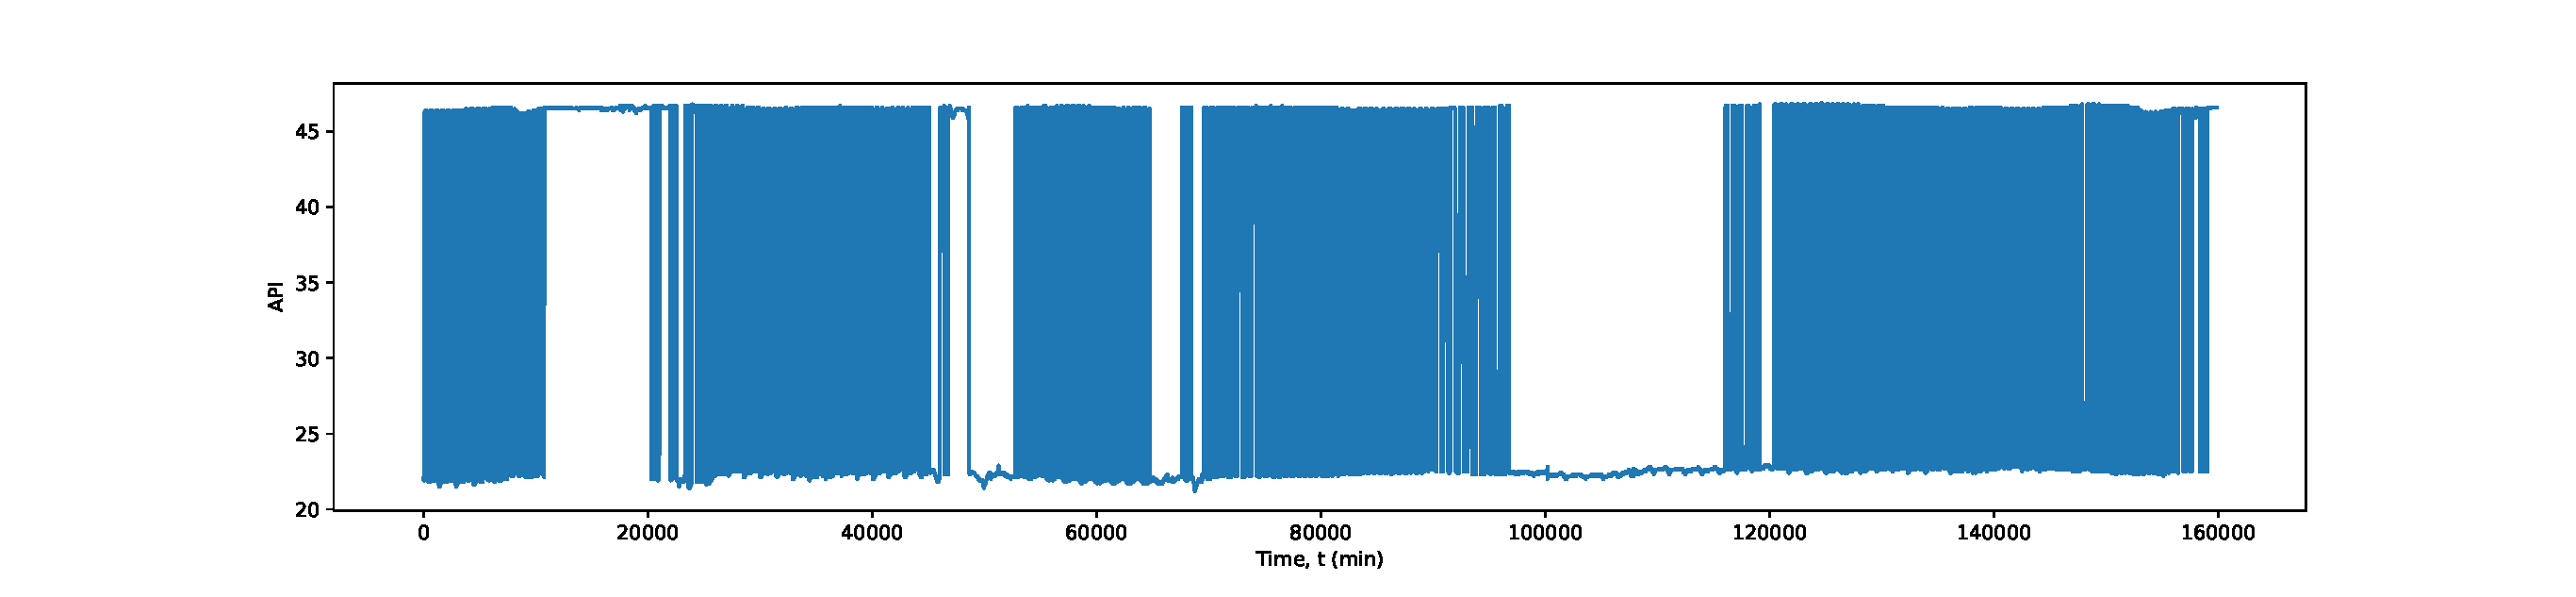
\includegraphics[width=\textwidth]{images/08NonFilteredDensity.eps}
         \caption{API data before abnormal condition removal.}
         \label{fig:08APIBefore}
     \end{subfigure}
     \hfill
     \begin{subfigure}[b]{1.0\textwidth}
         \centering
         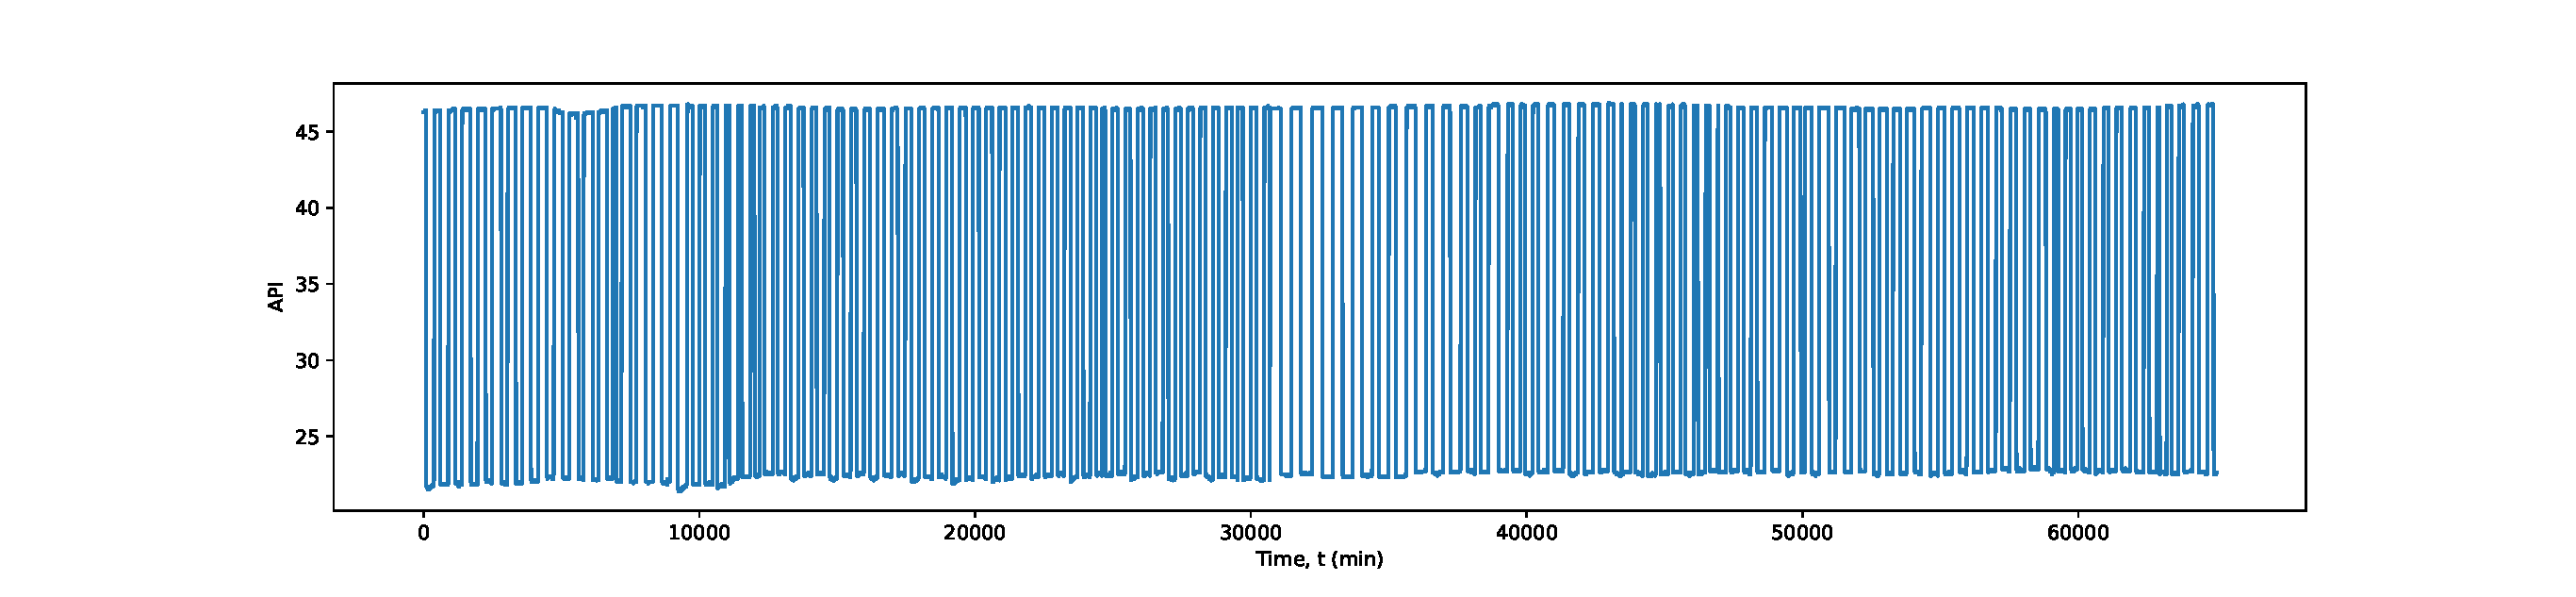
\includegraphics[width=\textwidth]{images/08FilteredDensity.eps}
         \caption{API data after abnormal condition removal.}
         \label{fig:08APIAfter}
     \end{subfigure}
        \caption{API data before and after removing abnormal operating conditions.}
        \label{fig:08API}
\end{figure}

Moreover, there is a time delay for the flow rate to react to a DRA set point change because the new DRA concentration must be transported throughout the line before its effect can be fully realized.  DRA is assumed to be catastrophically destroyed when passing through a pump; thus, DRA is only required to coat the pipeline between pump stations for its full effect to be exploited.  For CIG, it must coat the pipeline between CIG to Ault.  For Ault, the pipeline spanning between Ault and Fort Lupton must be coated.  Given the flow rate of the pipeline, it will take approximately ten hours to sufficiently coat the majority of the pipeline. Hence, data corresponding to transitional periods are removed. At times, transitional times may take longer; however, removing additional data will reduce the available data for model identification.  

Pre- and post-processed DRA parts per million (ppm) measurements are shown in Figure \ref{fig:08DRA}. DRA ppm is measured continuously for the control of the DRA injection pumps. However, the measurement is unreliable and corrupted with noise. Because DRA set points are rarely changed, an exponentially weighted moving average (EWMA) was applied to the DRA ppm readings for increased measurement reliability.  The EWMA formula and bias correction are given in Equations \ref{eq:08EWMA} and \ref{eq:08Bias_Correction}, respectively: 
\begin{equation}
    v_t = \beta v_{t - 1} + (1 - \beta) \theta_t, \; v_0 = 0
    \label{eq:08EWMA}
\end{equation}
\begin{equation}
    v_t \leftarrow \frac{v_t}{1 - \beta^t}, \forall v \in V
    \label{eq:08Bias_Correction}
\end{equation}
where $v_{t}$ is the exponentially weighted value at time $t$.  $\beta$ is the exponentially weighing factor.  Larger $\beta$ results in smoother results.  $\theta_t$ is the original value at time $t$. $V$ is a vector representing the exponentially weighted values before bias correction.

The objective of the machine learning model was to predict the flow rate at Commerce City.  However, there is a natural time delay between the time an equipment status changed and the corresponding impact on downstream flow rate.  Because the pipeline is fully loaded and the product is incompressible, pressure changes upstream will be propagated downstream at close to the speed of sound \cite{fluid_mechanics}.  Table \ref{tab:08TimeToCC} shows the time required for pressure to propagate down the pipeline starting from each pump station.  The pump data for each pump station was shifted accordingly to account for this time delay.  
\begin{table}[h]
    \centering
    {\setstretch{1.2}
    \begin{tabular}{ p{6cm} | c | c | c | c}
             &  Cheyenne & CIG & Ault & Fort Lupton \\
        \hline
        Time to Commerce City at speed of sound in liquids (1480 m/s) \cite{fluid_mechanics}
        &  1.7 min  &  1.5 min  &  1.0 min  &  0.45 min  \\
    \end{tabular}}
    \caption{Time required for pressure changes at each pump station to be realized at Commerce City.}
    \label{tab:08TimeToCC}
\end{table}
\begin{figure}
     \centering
     \begin{subfigure}[b]{0.9\textwidth}
         \centering
         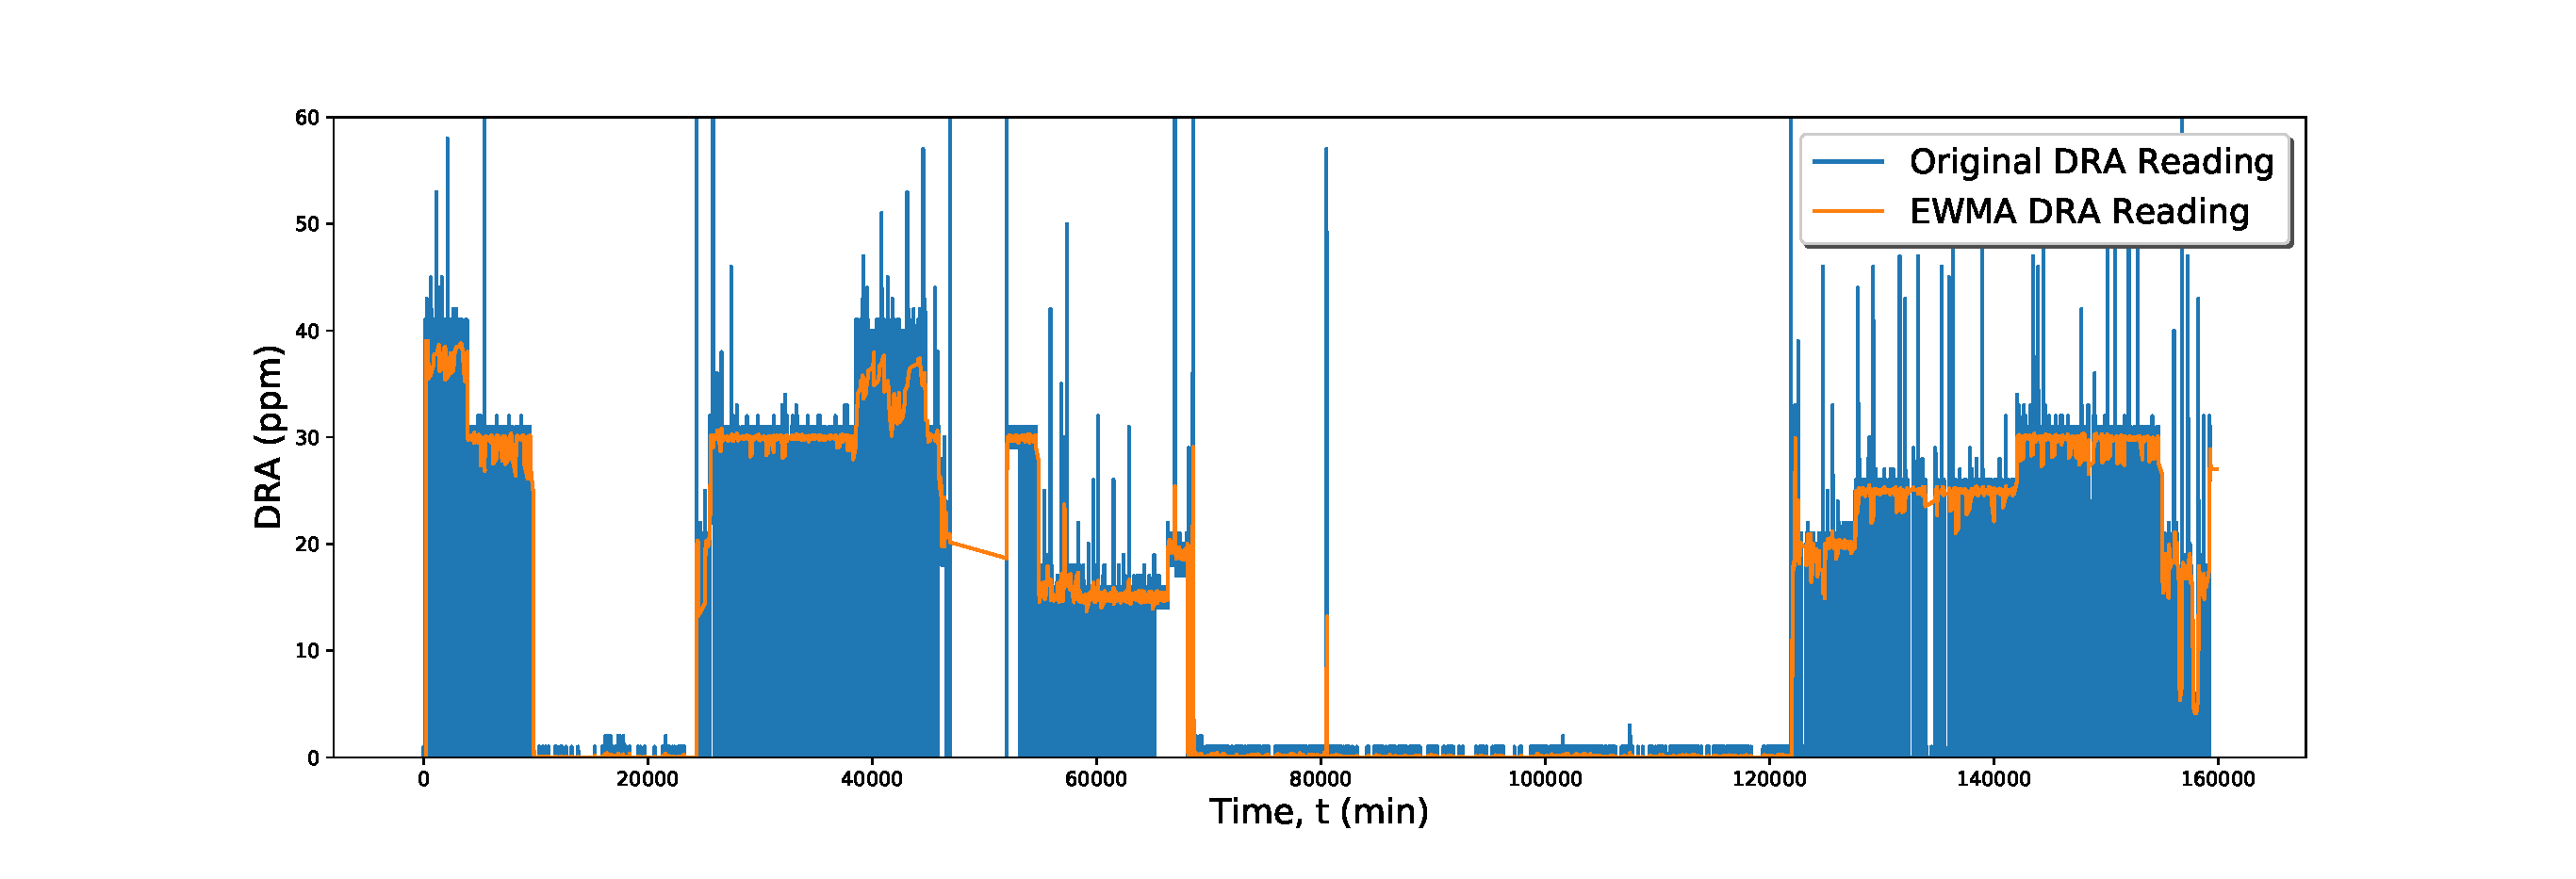
\includegraphics[width=\textwidth]{images/08CIGSour.eps}
         \caption{CIG sour DRA sensor reading.}
         \label{fig:08CIGSour}
     \end{subfigure}
     \begin{subfigure}[b]{0.9\textwidth}
         \centering
         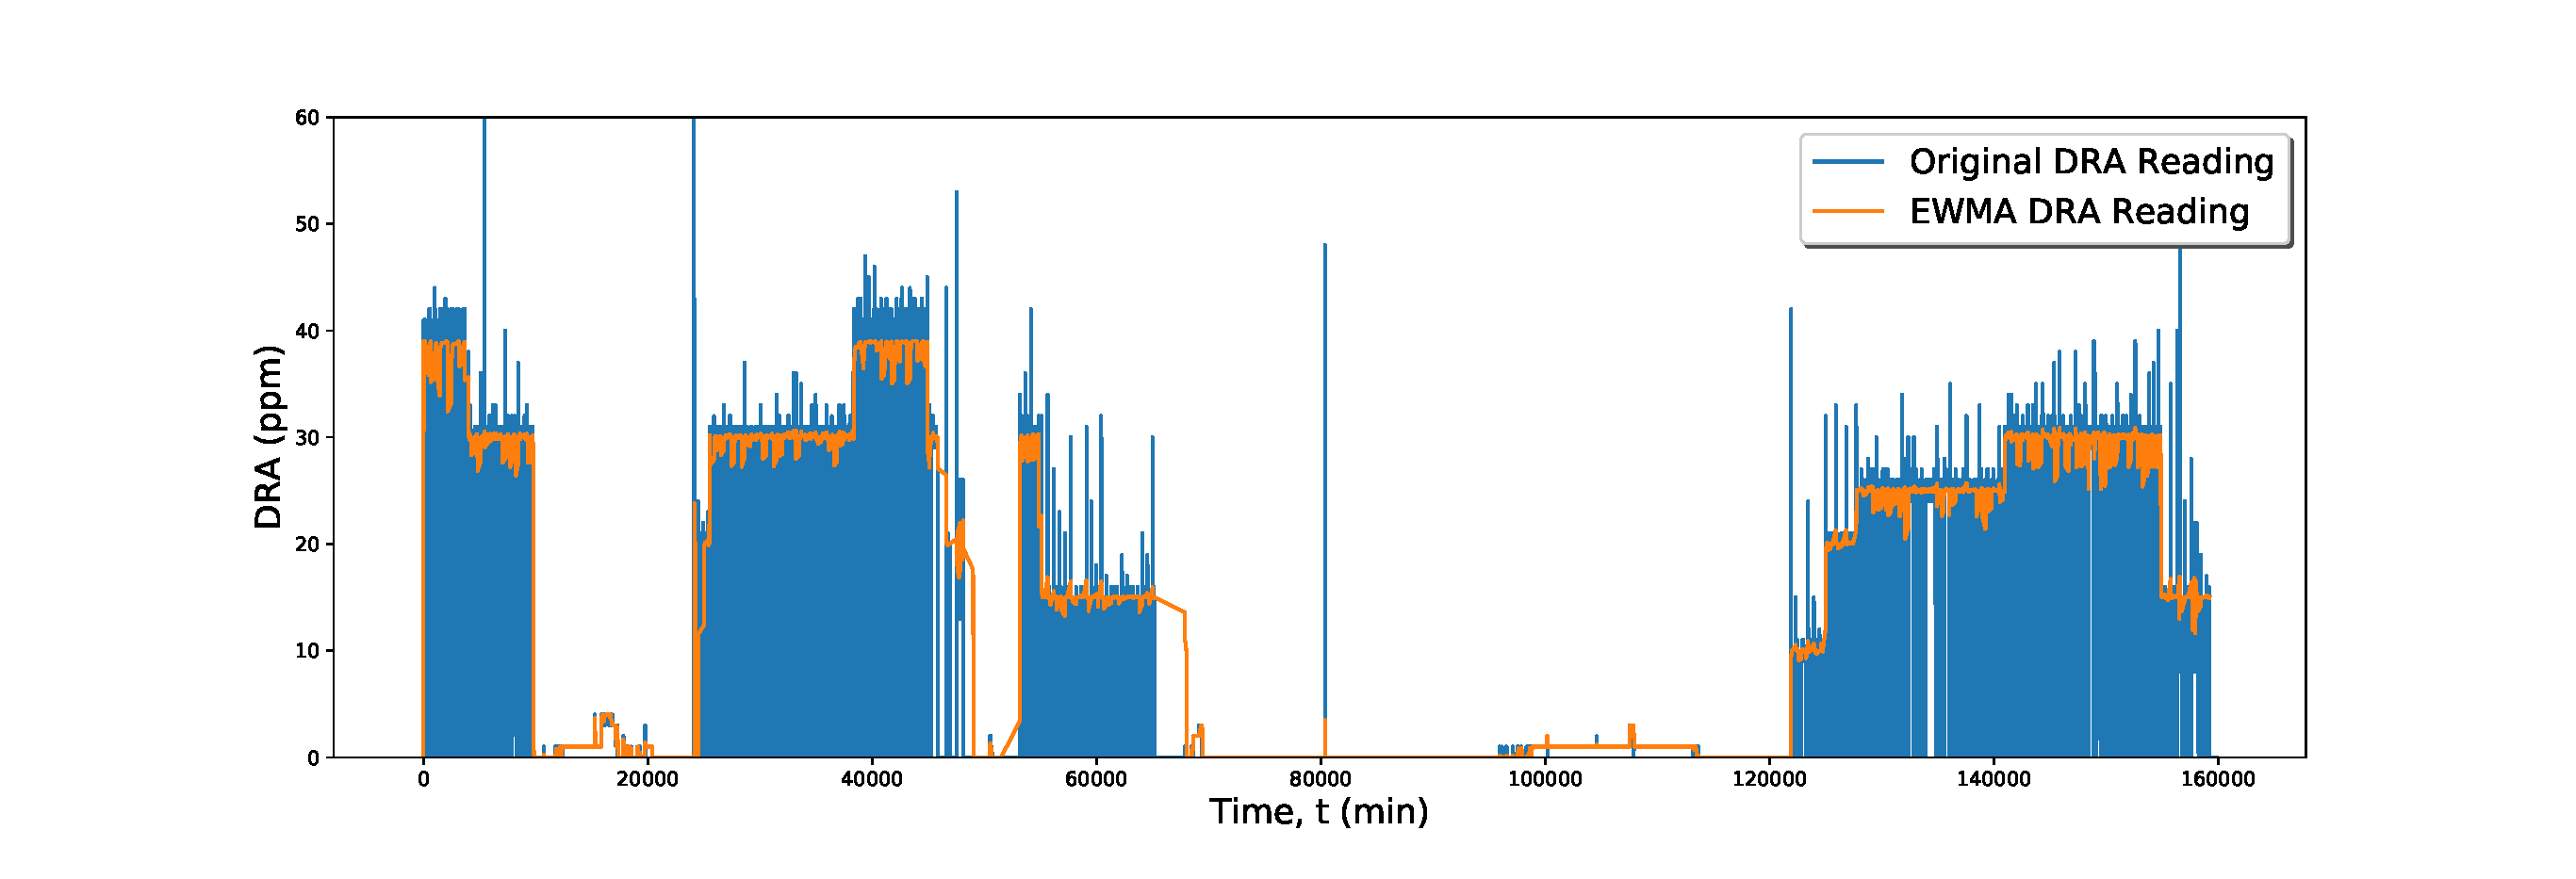
\includegraphics[width=\textwidth]{images/08CIGSweet.eps}
         \caption{CIG sweet DRA sensor reading.}
         \label{fig:08CIGSweet}
     \end{subfigure}
     \begin{subfigure}[b]{0.9\textwidth}
         \centering
         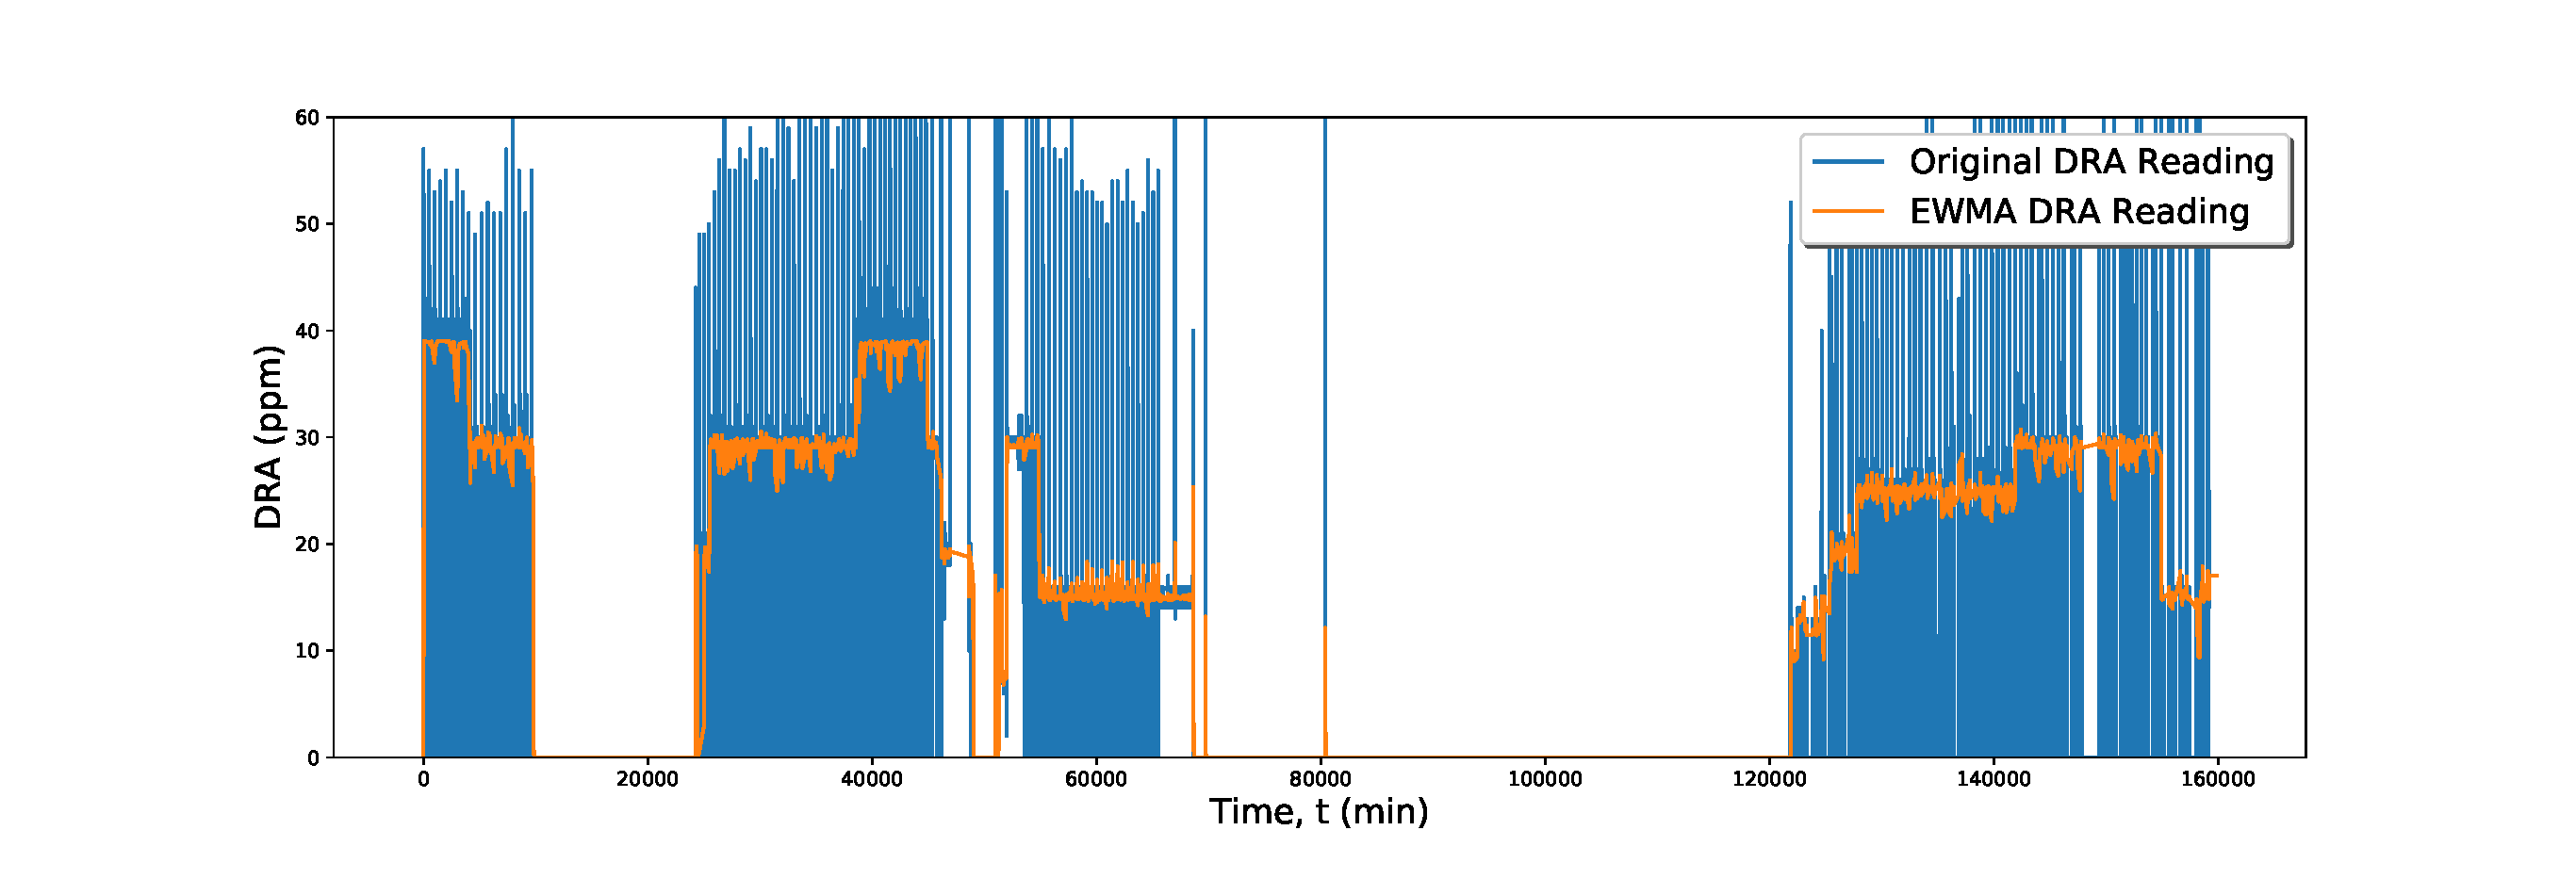
\includegraphics[width=\textwidth]{images/08AultSour.eps}
         \caption{Ault sour DRA sensor reading.}
         \label{fig:08AultSour}
     \end{subfigure}
     \begin{subfigure}[b]{0.9\textwidth}
         \centering
         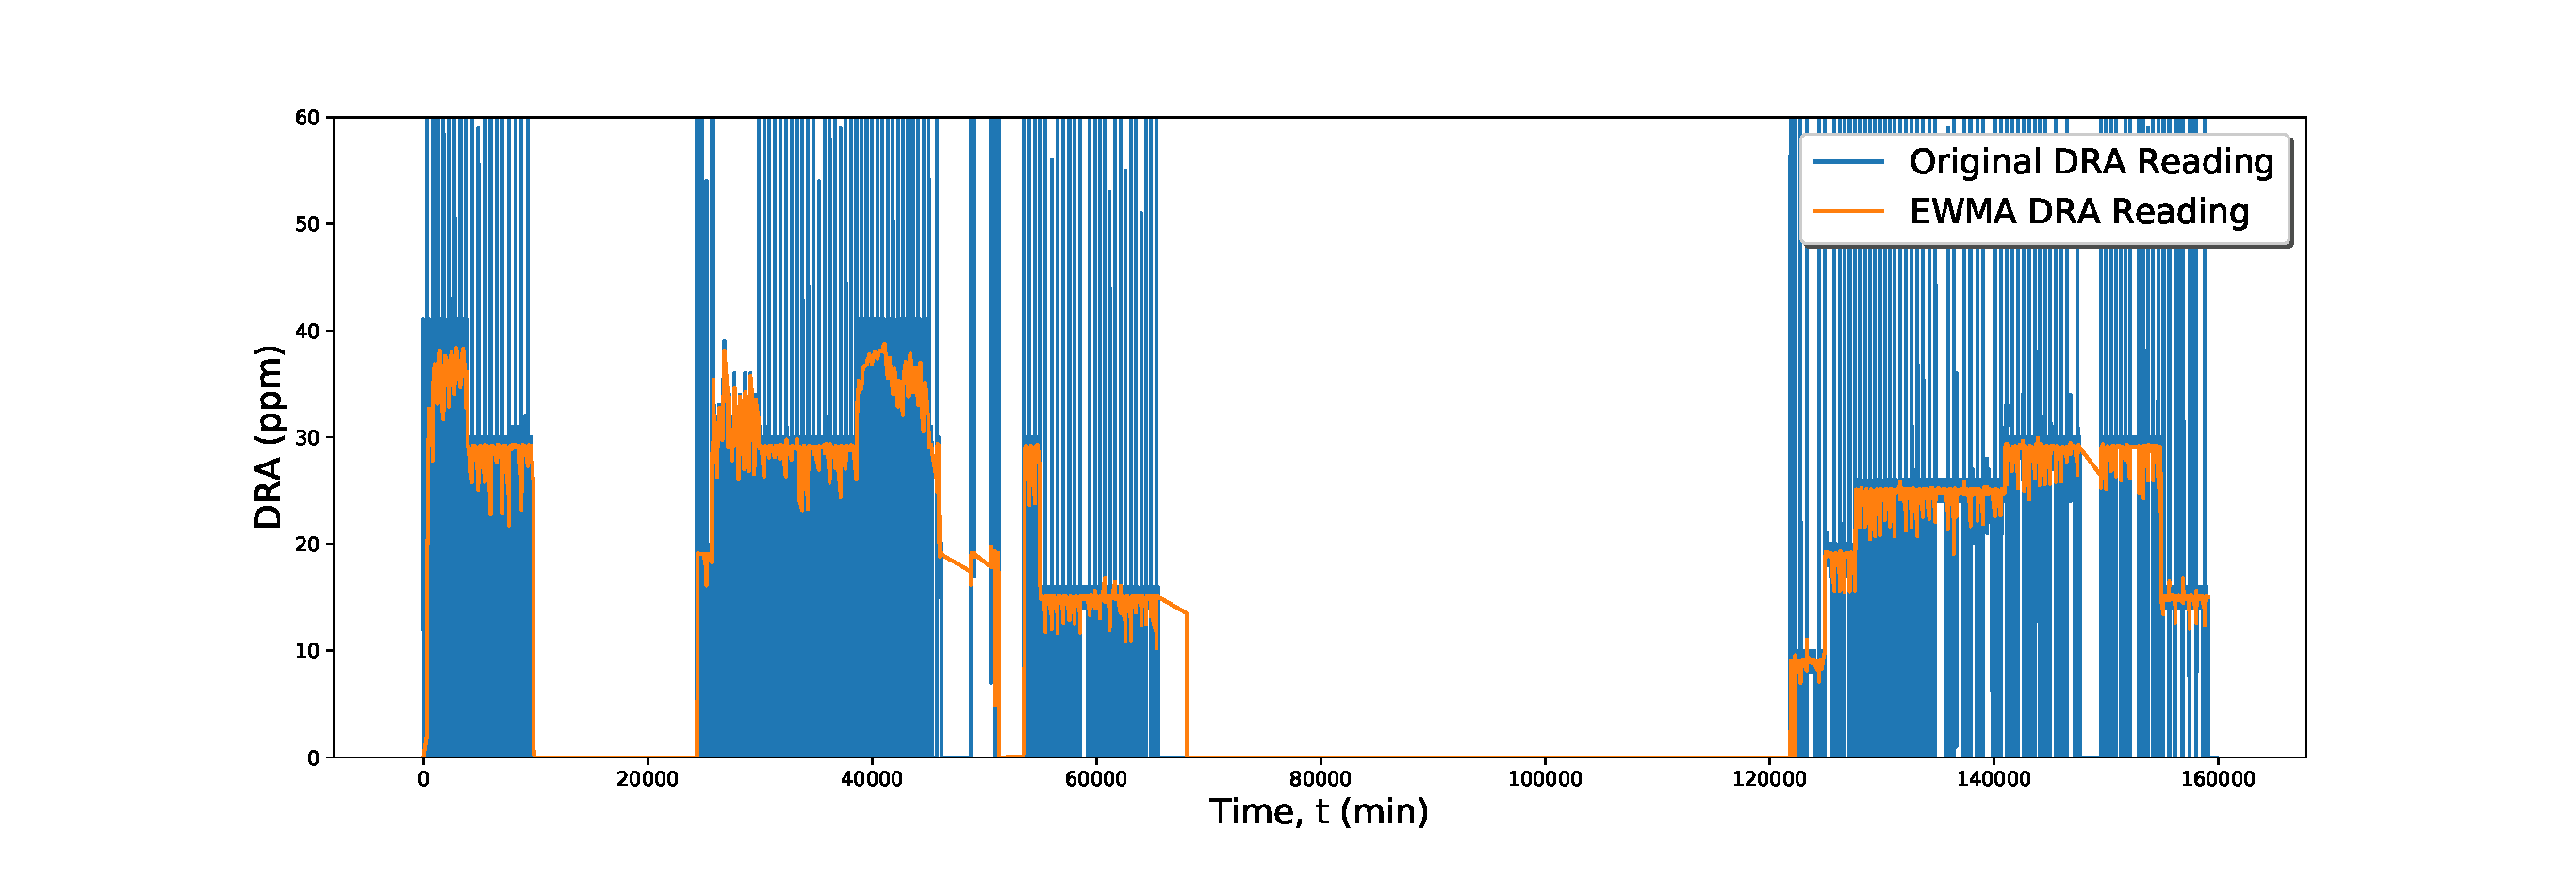
\includegraphics[width=\textwidth]{images/08AultSweet.eps}
         \caption{CIG sweet DRA sensor reading.}
         \label{fig:08AultSweet}
     \end{subfigure}
        \caption{Pre- and post-processed DRA sensor readings.}
        \label{fig:08DRA}
\end{figure}

A comprehensive list of the manual data pre-processing procedures is as follows:
\begin{enumerate}
    \item Shift data to accommodate the time delay at Commerce City.
    \item Smooth DRA data using exponentially weighted moving average given in Equation \ref{eq:08EWMA}.  
    \item Remove first 10 hours data corresponding to DRA set point changes.
    \item Remove data points where flow is under 800 bbl/hr.
    \item Remove data when only sweet or sour crude was sent through the pipeline.
\end{enumerate}

The final data set contained 65 variables and 97,470 data points.

\subsection{Model Identification}
\subsubsection{Feature Selection}
For each pump station, there was a variety of sensors measuring the same process variables.  For example, VFD pumps have four readings each: On/off status, RPM, HZ, and current. Many variables relating to one equipment is redundant; thus, only one variable was selected when redundancy existed. Additionally, some sensors were behaving abnormally.

In normal operations, the density fluctuates between 10 - 50 API, depending on the type of crude present in the pipeline.  After analysis, the Fort Lupton densitometer was behaving abnormally compared to other densitometer and is shown in Figure \ref{fig:08Density}.  After confirming with Suncor that the densitometer was behaving abnormally, the variable was removed.  
\begin{figure}[h]
     \centering
     \begin{subfigure}[b]{0.48\textwidth}
         \centering
         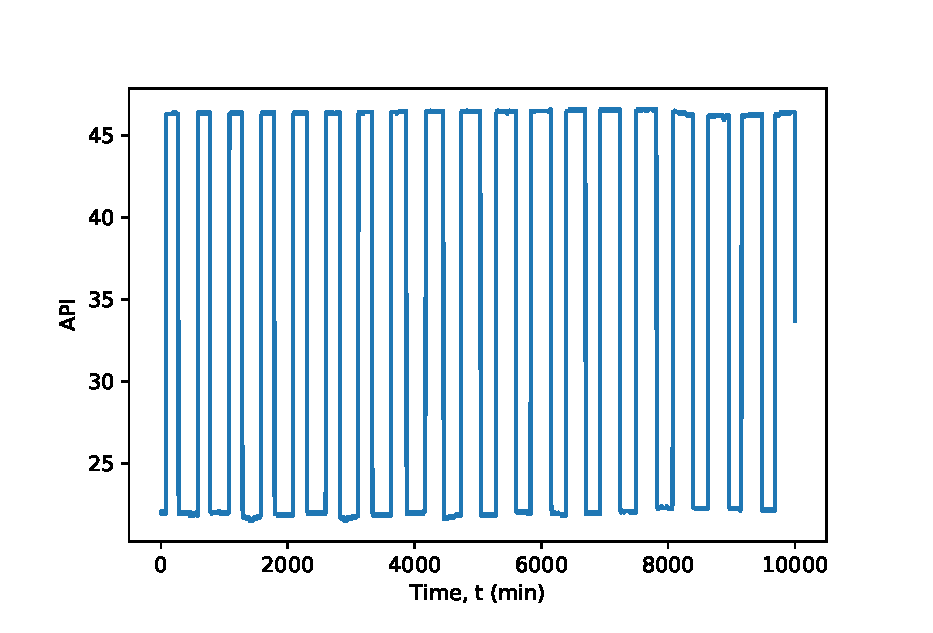
\includegraphics[width=\textwidth]{images/08CheyDensity.eps}
         \caption{Cheyenne API data for 10,000 mins.}
         \label{fig:08GoodDensity}
     \end{subfigure}
     \hfill
     \begin{subfigure}[b]{0.48\textwidth}
         \centering
         \includegraphics[width=\textwidth]{images/08FLDensity.eps}
         \caption{Fort Lupton API data for 10,000 mins.}
         \label{fig:08BadDensity}
     \end{subfigure}
        \caption{Comparison of normal and abnormal density readings.}
        \label{fig:08Density}
\end{figure}

Table \ref{tab:08featselect} shows the features selected for each pump station. The predicted variable was the flow rate (bbl/h) at Commerce City.
\begin{table}[h]
    \centering
    {\tiny
    {\setstretch{1.2}
    \begin{tabular}{ c | c | c | c | c}
        Cheyenne                       & CIG                      & Ault                        & Fort Lupton                    & Commerce City \\
        \hline
        $u_5$: Boos. Pump Status       &  $u_1$: Sweet DRA (ppm)  &  $u_3$: Sweet DRA (ppm)     &  $u_{8}$: Boos. Pump Status   &  $x_{8}$: Inlet Temp. (°C) \\
        
        $u_9$: VFD Current (Amp)       &  $u_2$: Sour DRA (ppm)   &  $u_4$: Sour DRA (ppm)      & $u_{10}$: VFD Current (Amp)      & \\
        
        $x_{4}$: Inlet Temp. (°C)     &  $x_{5}$: Inlet Temp. (°C) &  $u_6$: Small Pump Status &  $x_{7}$: Inlet Temp. (°C)  & \\
        
        $x_{1}$: API                   &  $x_{2}$: API          &  $u_7$: Large Pump Status   &             
        & \\
        
                                       &                          &  $x_{6}$: Inlet Temp. (°C)  &             
        & \\
        
                                       &                          &  $x_{3}$: API               &       
        & \\
        
    \end{tabular}}}
    \caption{Features selected for machine learning models.}
    \label{tab:08featselect}
\end{table}

\subsubsection{Feature Scaling}
Figure \ref{fig:08featscale} shows the contour of a normalized and non-normalized cost function. It can be seen that the optimization of a non-normalized cost function can be significantly hindered depending on where the optimization is initialized.

\begin{figure}[h]
    \centering
    \includegraphics[width=.8\textwidth]{images/08featscale.png}
    \caption{Coutour of normalized and non-normalized cost functions. Original images from \cite{deeplearning_course}.}
    \label{fig:08featscale}
\end{figure}

To avoid this problem, the min-max normalization is applied to each variable and is given by:
\begin{equation}
    x^{norm} = \frac{x - x^{min}}{x^{max} - x^{min}}
    \label{eq:08normalization}
\end{equation}
where $x^{norm}$ is the normalized values.  Here, $x^{min}$ and $x^{max}$ are the minimum and maximum values of each variable, respectively.  By applying this normalization, all data will be bounded between $x_i \in [0, 1]$ and the elongation issue of the cost function will be resolved.

\subsubsection{Exploratory Data Analysis}
Exploratory data analysis was then conducted to gain insights into the data set.  First, the distribution of the flow rate was explored and shown in Figure \ref{fig:08flowrate_dist}.  It can be seen that the flow rate follows a bi-modal distribution corresponding to two different operating strategies: a high demand strategy and a low demand strategy.

\begin{figure}[h]
    \centering
    \includegraphics[scale=0.35]{images/08Flowrate_KDE.eps}
    \caption{Flow rate distribution of the pre-processed data set.}
    \label{fig:08flowrate_dist}
\end{figure}

To segregate the two Gaussian distributions, DBSCAN was used.  DBSCAN is a density-based algorithm for discovering clusters in large spatial data \cite{DBSCAN}. DBSCAN also scales much better to big data compared to affinity propagation or Gaussian mixture models due to the latter being iterative methods.
DBSCAN contains two hyper parameters, $\epsilon$ and $min \; points$.  The steps of DBSCAN is as follows:
\begin{enumerate}
    \item Normalize the data using Equation \ref{eq:08normalization} so each variable is weighted similarily.
    \item Create an $n-$dimensional sphere of radius $\epsilon$ around an initial data point.  Euclidean distance was used for the distance metric and is given by:
    \begin{equation}
        distance = \sqrt{(x_1^{(1)} - x_1^{(2)})^2 + (x_2^{(1)} - x_2^{(2)})^2 + ... + (x_m^{(1)} - x_m^{(2)})^2}
    \end{equation}
    where superscripts $1$ and $2$ denotes the first and second data points.
    \item If there are more than $min \; points$ in this sphere, then all points within this sphere belong to the same cluster.
    \item Expand the cluster by recursively applying the above criteria to the edge points of the cluster.
    \item If the cluster can no longer be expanded, apply steps 2 - 4 to a new data point currently not belonging to a cluster.
    \item If there are less than $min \; points$ in this sphere, then the data point is ignored and we proceed to the next data point.
    \item Outlier data points are ones that fail to belong to any cluster.
\end{enumerate}
The resultant segregation created by DBSCAN using hyper parameters 1.13 and 10,000 for $\epsilon$ and $min \; points$ is shown in Figure \ref{fig:08DBSCAN}. The first cluster (black) contained 56,738 data points while the second cluster (green) contained 36,779 data points.  The remaining 3953 data points (blue) were identified as outliers.
\begin{figure}[h]
    \centering
    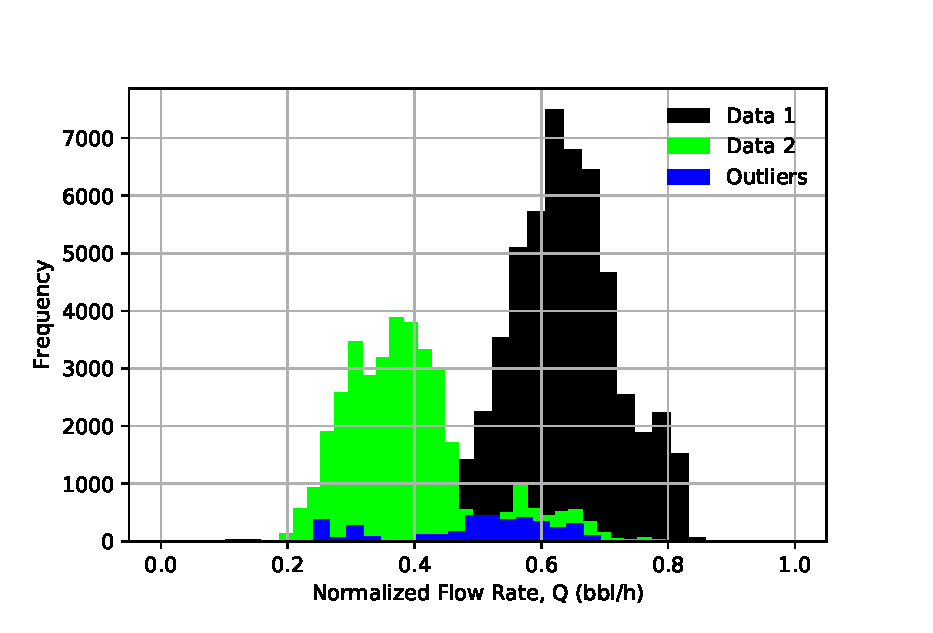
\includegraphics[scale=0.8]{images/08DBSCAN.eps}
    \caption{Clusters identified after applying the density-based scan.}
    \label{fig:08DBSCAN}
\end{figure}

The average operating conditions of each cluster is shown in Figure \ref{fig:08cluster_variables}. The main differences are the flow rate, DRA usage, and pump usage.  Cluster 1 had 32\% higher average flow rate.  Cluster 1 also used substantially more DRA compared to cluster 1, where almost no DRA was used. Furthermore, the Cheyenne booster pump, Ault booster pump 1, Fort Lupton boooster pump, and Fort Lupton VFD were only used in cluster 1.  Ault booster pump 2 was only used in cluster 2.
\begin{figure}
    \centering
    \includegraphics[width=0.8\textwidth]{images/08AvgChar.png}
    \caption{Average operating variables for the two operating conditions.}
    \label{fig:08cluster_variables}
\end{figure}

\subsubsection{Data Partitioning}
The data set was split into three sections for machine learning: training, validation, and testing.  The partition and description of each section is described in Table \ref{tab:08datapart}. The training data set was used to identify the machine learning model(s).  Then, the model was validated on unseen data via the validation data set (sometimes called development data).  The error of the model on the validation data set, $e_{validation}$, should be similar to the training data error, $e_{train}$, to ensure that the model did not overfit to the training data. Finally, the model will be tested on the testing data to explore the performance of the model in live production.  Testing data will always be the last 5\% of the data in the data set.
\begin{table}[h]
    \centering
    {\setstretch{1.2}
    \begin{tabular}{ c | c | p{9cm}}
                            & \% of Data        &  Description \\
        \hline
        Training            &  90\%             
        &  Used to identify the machine learning model        \\
        
        Validation          &  5\%              
        &  Validates the performance of the machine learning model         \\
        
        Testing             &  5\%             
        &  Used to test performance of machine learning model on unseen data       \\             
    \end{tabular}}
    \caption{Features selected for machine learning models.}
    \label{tab:08datapart}
\end{table}

\subsubsection{Cost Function}

The mean squared error (MSE) cost function was used for all predictive models and is given by:
\begin{equation}
    J(W) = \frac{1}{n}\sum\limits^n_{i=1}(\hat{y}_i - y_i)^2
    \label{eq:08MSE}
\end{equation}
where $n$ is the number of samples in the current optimization step.  $\hat{y}_i$ and $y_i$ are the $i^{th}$ predicted and actual labels, respectively. Here, $J$ is the loss. The MSE cost function was selected due to its convex nature \cite{deeplearning_course}.

To ensure adequate performance on the validation and testing data, the model must avoid overfitting to the training data.  This was done by reducing the model complexity through removing or reducing individual variables' impact on the model.  This study used a ridge regularization to reduce model complexity:
\begin{equation}
    J(W) = \frac{1}{n}\sum\limits^n_{i=1}(\hat{y}_i - y_i)^2 + \lambda \sum\limits^n_{j=1} W_j^2
    \label{eq:08MSE_wR}
\end{equation}
where $\lambda$ is the regularization penalty.  Here, as $\lambda \rightarrow \infty$, $W \rightarrow 0$.  That is, the larger $\lambda$ is, the stronger the weights are penalized. 

\subsubsection{Model Optimization}

The adaptive momentum (ADAM) gradient descent optimizer was used to update the weights and bias of the models.  The general gradient descent formulation is given by Equation \ref{eq:08GradientDescent} \cite{ADAM}.  
\begin{equation}
    \theta_j^{m+1} \leftarrow \theta_j^{m} - \alpha \frac{\partial J}{\partial \theta_j}
    \label{eq:08GradientDescent}
\end{equation}
where $\theta_j$ is the $j^{th}$ weight of the model.  Here, $m$ represents the $m^{th}$ update of gradient descent and $\alpha$ is the learning rate.  ADAM improves upon Equation \ref{eq:08GradientDescent} by computing an adaptive learning rate for each parameter. To do so, the exponentially decaying average of the past gradients and squared gradients of the weights and biases are computed and stored using Equations \ref{eq:08momentW} to \ref{eq:08squared_momentb}.
\begin{equation}
    V_{dW} = \beta_1 V_{dW} + (1 - \beta_1)dW
    \label{eq:08momentW}
\end{equation}
\begin{equation}
    V_{db} = \beta_1 V_{db} + (1 - \beta_1)db
    \label{eq:08momentb}
\end{equation}
\begin{equation}
    S_{dW} = \beta_2 S_{dW} + (1 - \beta_2)dW^2
    \label{eq:08squared_momentW}
\end{equation}
\begin{equation}
    S_{db} = \beta_2 S_{db} + (1 - \beta_2)db^2
    \label{eq:08squared_momentb}
\end{equation}
where $V$ and $S$ are the estimates of the gradient and squared gradients, respectively.  $V$ and $S$ are typically initiated as zero vectors and are heavily biased towards zero at initial steps.  Hence, the biases for the initial terms are corrected using:
\begin{equation}
    V_{dW}^{corrected} = \frac{V_{dW}}{1 - \beta_1^t}
\end{equation}
\begin{equation}
    V_{db}^{corrected} = \frac{V_{db}}{1 - \beta_1^t}
\end{equation}
\begin{equation}
    S_{dW}^{corrected} = \frac{S_{dW}}{1 - \beta_2^t}
\end{equation}
\begin{equation}
    S_{db}^{corrected} = \frac{S_{db}}{1 - \beta_2^t}
\end{equation}
Combining the above equations, the weights and biases are updated by:
\begin{equation}
    W_j \leftarrow W_j - \alpha \frac{V_{dW}^{corrected}}{S_{dW}^{corrected} + \epsilon}
\end{equation}
\begin{equation}
    b \leftarrow b - \alpha \frac{V_{db}^{corrected}}{S_{db}^{corrected} + \epsilon}
\end{equation}
where $\epsilon$ is a small scalar to avoid division by zero. The authors proposed values of 0.9, 0.999 and $10^{-8}$ for $\beta_1$, $\beta_2$, and $\epsilon$, respectively.

Due to the size of the data, batch gradient descent where all data are used to compute the gradient at each step is computationally infeasible.  Thus, mini-batch gradient descent was used where smaller batches of data were sampled from the original data set to perform stochastic updates at each step.
\subsubsection{Performance Assessment}
The model performance were assessed using the following three ways:
\begin{enumerate}
    \item Root mean squared error (RMSE):
    \begin{equation}
        J = \sqrt{\frac{1}{n}\sum\limits^n_{i=1}(\hat{y}_i - y_i)^2}
        \label{eq:08RMSE}
    \end{equation}
    
    \item Mean absolute error (MAE):
    \begin{equation}
        J = \frac{1}{n}\sum\limits^n_{i=1}|\hat{y}_i - y_i|
        \label{eq:08MSE_Error}
    \end{equation}
    \item Coefficient of determination ($R^2$):
    \begin{equation}
        R^2 = 1 - \frac{\sum\limits^n_{i = 1}(\hat{y_i} - y_i)^2}{\sum\limits^n_{i = 1}(y_i - \bar{y_i})^2}
    \end{equation}
\end{enumerate}
Table \ref{tab:08performanceassessment} shows the advantages and disadvantages of each assessment metric.
\begin{table}[h]
    \centering
    {\setstretch{1.2}
    \begin{tabular}{ c | p{7cm} | p{7cm}}
         Method             & Advantages        &  Disadvantages \\
        \hline
        RMSE                &  Useful for identifying large errors                            &  Smaller errors are muted        \\
        
        MAE                 &  Easy to interpret as all errors have the same weight           &  Inferior to RMSE when large errors are undesirable \\
        
        $R^2$               &  Easy to understand, $-\infty \leq R^2 \leq 1$                                         &  Valid only for linear relationships       \\             
    \end{tabular}}
    \caption{Constrained least squares validation and test plots.}
    \label{tab:08performanceassessment}
\end{table}

%%%%%%%%%%%%%%%%%%%%%%%%%%%%%%%%%%%%%%%%%%%%%%%%%%%%%%%%%%%%%%%%%%%%%
%
% Least squares model
%
%%%%%%%%%%%%%%%%%%%%%%%%%%%%%%%%%%%%%%%%%%%%%%%%%%%%%%%%%%%%%%%%%%%%%
\subsubsection{Linear Modelling}
\noindent
\textit{Linear Regression} \\
Linear regression was the first regression method to be explored, and was selected as the benchmark due to its simplicity and linear nature. The model structure of linear regression is given as:
\begin{equation}
    \hat{y} = W_1^Tx + W_2^Tu + b
    \label{eq:08LS}
\end{equation}
where $x \in R^8$ is a vector of states, $u \in R^{10}$ is a vector of inputs and superscript $T$ denotes the transpose operation.

Hyper parameters of the linear regression are shown in Table \ref{tab:08LSHparameters}.
\begin{table}[h]
    \centering
    {\setstretch{1.2}
    \begin{tabular}{ c | c}
        Hyper Parameter                  &  Value       \\
        \hline
        Epochs                           &  800      \\
        Minibatch size                   &  8192     \\
        Learning rate, $\alpha$          &  0.001    \\
        Regularization, $\lambda$          &  0.001  \\
    \end{tabular}}
    \caption{Hyper parameters for linear regression.}
    \label{tab:08LSHparameters}
\end{table}

The performance assessment of the least squares model is shown in Table \ref{tab:08LSperformance}. Error on the test data was 5.8\% higher compared to the training and validation data.
\begin{table}[h]
    \centering
    {\setstretch{1.2}
    \begin{tabular}{ c | c | c | c}
                             &  Training data    &  Validation data   &    Test data      \\
        \hline
        MAE                  &  98               &    98              &  102     \\
        RMSE                 &  127              &   127              &  135    \\ 
        $R^2$                &  0.91             &   0.91             &  0.70   \\
    \end{tabular}}
    \caption{Performance assessment for the linear regression.}
    \label{tab:08LSperformance}
\end{table}

The model performance on the validation and test data sets are shown in Figures \ref{fig:08LSValidation} and \ref{fig:08LSTest}.
\begin{figure}[h]
     \centering
     \begin{subfigure}[b]{0.48\textwidth}
         \centering
         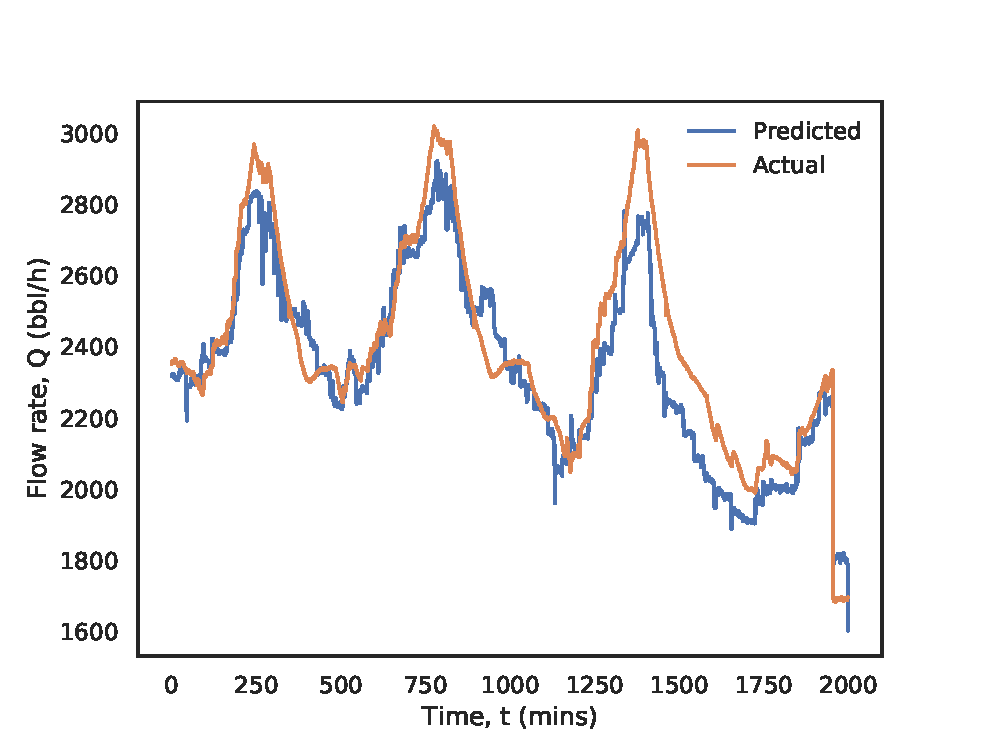
\includegraphics[width=\textwidth]{images/08ls_validation.eps}
         \caption{Predicted vs. actual flow rate for the validation data set.}
         \label{fig:08LSValidation}
     \end{subfigure}
     \hfill
     \begin{subfigure}[b]{0.48\textwidth}
         \centering
         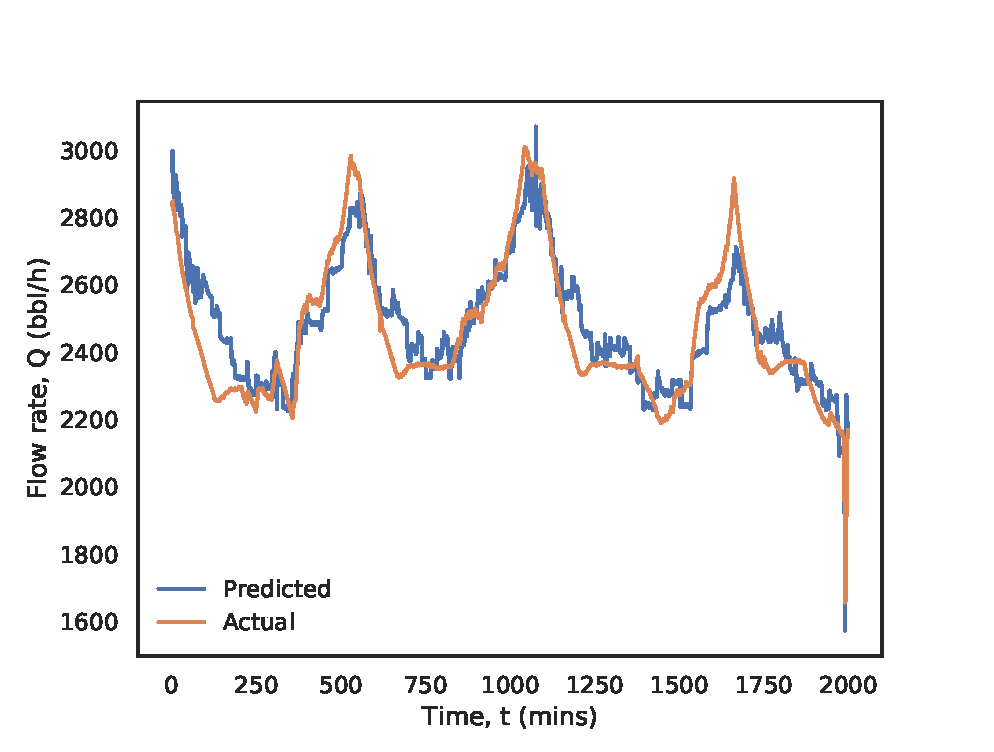
\includegraphics[width=\textwidth]{images/08ls_test.eps}
         \caption{Predicted vs. actual flow rate for the test data set.}
         \label{fig:08LSTest}
     \end{subfigure}
        \caption{Comparison of normal and abnormal density readings.}
        \label{fig:08LSPlots}
\end{figure}

The linear regression model is given in Equation \ref{eq:08LS}.  Weights for $x_{1} - x_{4}$ were very small and were omitted.
\begin{multline}
    \hat{y} = 0.10u_1 + 0.15u_2 + 0.13u_3 + 0.04u_4 + 0.04u_5 + 0.09u_6 + 0.12u_7 - 0.01u_8 \\
    + 0.49u_9 + 0.02u_{10} + 0.09x_{1} - 0.18x_{5} + 0.30x_{6} - 0.05x_{7} + 0.04x_{8}
    \label{eq:08LS_eq}
\end{multline}

From Equation \ref{eq:08LS}, it can be seen that turning on the booster pump at Fort Lupton results in a decrease in flow rate.  Theoretically, this is impossible and is most likely caused by noise in the data.  To increase the model's ability to reflect reality, engineering knowledge was injected into the model via constraining the weights of $u_1 - u_{10}$ to be strictly positive.

%%%%%%%%%%%%%%%%%%%%%%%%%%%%%%%%%%%%%%%%%%%%%%%%%%%%%%%%%%%%%%%%%%%%%
%
% Constrained LS
%
%%%%%%%%%%%%%%%%%%%%%%%%%%%%%%%%%%%%%%%%%%%%%%%%%%%%%%%%%%%%%%%%%%%%%

\noindent
\textit{Constrained Linear Regression} \\
\indent
The constrained linear regression used the same hyper parameters as shown in Table \ref{tab:08LSHparameters}.  Performance assessment of the constrained linear regression is shown in Table \ref{tab:08ConstLSPerformance}. Compared to the original linear regression, RMSE increased by 0.8\% for the training and validation data sets.  However, performance on the test set was improved by 8\%.  
\begin{table}[h]
    \centering
    {\setstretch{1.2}
    \begin{tabular}{ c | c | c | c}
                             &  Training data    &  Validation data   &    Test data      \\
        \hline
        MAE                  &  98               &    98              &  94     \\
        RMSE                 &  128              &   129              &  123    \\ 
        $R^2$                &  0.91             &   0.91             &  0.74   \\
    \end{tabular}}
    \caption{Performance assessment for the constrained linear regression.}
    \label{tab:08ConstLSPerformance}
\end{table}
The constrained linear regression performance on the validation and test data sets are shown in Figures \ref{fig:08CLSValidation} and \ref{fig:08CLSTest}. The weights were nearly identical to the unconstrained model; however, all negative weights on operating variables were removed.
\begin{figure}[h]
     \centering
     \begin{subfigure}[b]{0.48\textwidth}
         \centering
         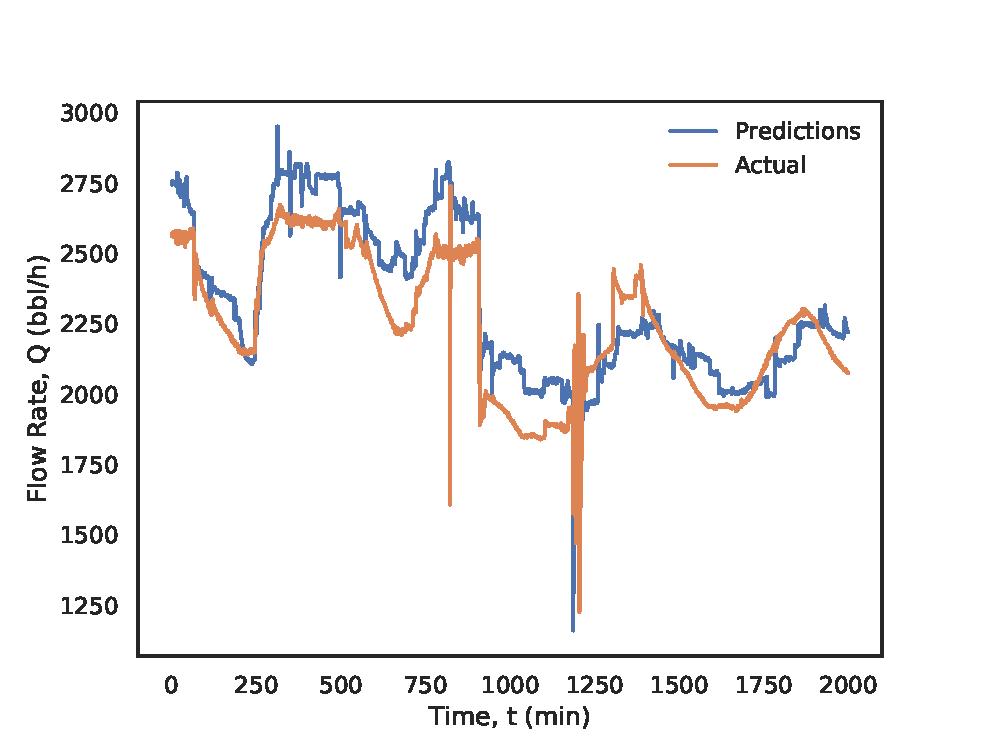
\includegraphics[width=\textwidth]{images/08ConstrainedLS_validation.eps}
         \caption{Predicted vs. actual flow rate for the validation data set.}
         \label{fig:08CLSValidation}
     \end{subfigure}
     \hfill
     \begin{subfigure}[b]{0.48\textwidth}
         \centering
         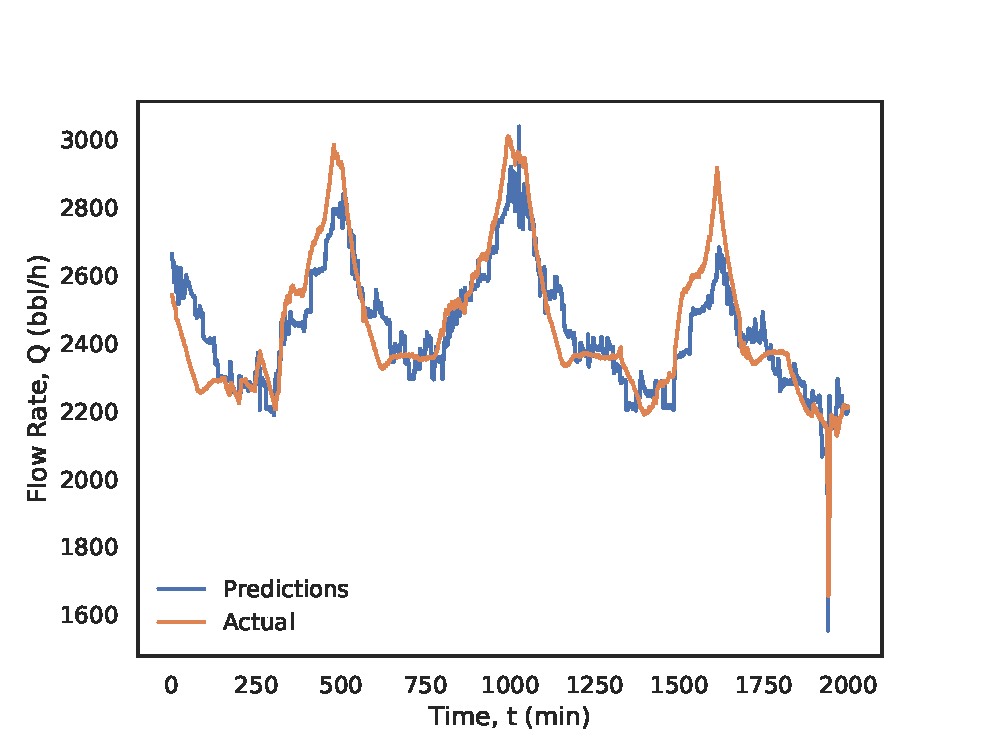
\includegraphics[width=\textwidth]{images/08ConstrainedLS_test.eps}
         \caption{Predicted vs. actual flow rate for the test data set.}
         \label{fig:08CLSTest}
     \end{subfigure}
        \caption{Constrained linear regression validation and test plots.}
        \label{fig:08CLSPlots}
\end{figure}

The constrained linear regression is given in Equation \ref{eq:08CLS}.  Weights for $x_{8}, x_{11} - x_{14}$ were very small and were omitted.
\begin{multline}
    \hat{y} = 0.10x_1 + 0.15x_2 + 0.13x_3 + 0.04x_4 + 0.04x_5 + 0.09x_6 + 0.11x_7 \\
    + 0.49x_9 + 0.02x_{10}  - 0.18x_{15} + 0.30x_{16} - 0.05x_{17} + 0.03x_{18}
    \label{eq:08CLS}
\end{multline}

\subsubsection{Non-linear Modelling}
To further increase the accuracy of the models, the following non-linear methods were explored for modelling the pipeline flow rate:
\begin{itemize}
    \item Polynomial models
    \begin{itemize}
        \item Quadratic model
        \item Square-root model
    \end{itemize}
    \item Feed-forward neural networks
    \begin{itemize}
        \item Small neural network (3 layers, 20 nodes per layer)
        \item Medium neural network (6 layers, 30 nodes per layer)
        \item Large neural network (8 layers, 40 nodes per layer)
    \end{itemize}
    \item Linear parameter-varying model
\end{itemize}

Performance assessment of the non-linear models will use MAE and RMSE. In non-linear models, $R^2$ is not valid due to $SS_R + SS_E \neq SS_{Total}$ and was not provided \cite{generic_stats}.
%%%%%%%%%%%%%%%%%%%%%%%%%%%%%%%%%%%%%%%%%%%%%%%%%%%%%%%%%%%%%%%%%%%%%
%
%  Quadratic and Sqrt models
%
%%%%%%%%%%%%%%%%%%%%%%%%%%%%%%%%%%%%%%%%%%%%%%%%%%%%%%%%%%%%%%%%%%%%%
\noindent
\textit{Polynomial Models} \\
The quadratic and square-root model structures are given by Equations \ref{eq:08quad_model} and \ref{eq:08sqrt_model}, respectively:
\begin{equation}
    \hat{y} = W_1^T X^2 + W^T_2 X + b
    \label{eq:08quad_model}
\end{equation}
\begin{equation}
    \hat{y} = W_1^T X^{1/2} + W^T_2 X + b
    \label{eq:08sqrt_model}
\end{equation}
where $W_1 \in R^{18}$ are the weights for the squared and square rooted variables for the quadratic and square root models, respectively. Furthermore, $W_2 \in R^{18}$ are the weights for the original variables. The hyper parameters for both models are shown in Table \ref{tab:08poly_hp}.
\begin{table}[h]
    \centering
    {\setstretch{1.2}
    \begin{tabular}{ c | c}
        Hyper Parameter                  &  Value       \\
        \hline
        Epochs                           &  1000      \\
        Minibatch size                   &  8192     \\
        Learning rate, $\alpha$          &  0.001    \\
        Regularization, $\lambda$          &  0.001  \\
    \end{tabular}}
    \caption{Hyper parameters for polynominal regression.}
    \label{tab:08poly_hp}
\end{table}

The performance assessment of the quadratic and square root models are shown in Table \ref{tab:08quad_sqrt_performance}. Compared to linear regression, MAE and RMSE reduced by up to 10\% and 9\% when using the polynomial models, respectively. Moreover, performance of the square root model was about 3.5\% better than the quadratic model.
\begin{table}[h]
    \centering
    {\setstretch{1.2}
    \begin{tabular}{c|c|c|c|c|c|c|}
      & \multicolumn{2}{c|}{Training data} & \multicolumn{2}{c|}{Validation data} & \multicolumn{2}{c|}{Test data} \\ \cline{2-7} 
      & Quad             & Sqrt            & \multicolumn{1}{c|}{Quad}   & Sqrt   & Quad           & Sqrt          \\ \hline
    MAE   & 92               & 89              & 92                          & 89     & 89             & 91            \\
    RMSE  & 121              & 118             & \multicolumn{1}{c|}{121}    & 117    & 120            & 115           \\
    \end{tabular}}
    \caption{Performance assessment for the quad. and sqrt. model.}
    \label{tab:08quad_sqrt_performance}
\end{table}

The polynomial models' performance on the validation and test data are shown in Figures \ref{fig:08quad_validation} to \ref{fig:08sqrt_test}.  

\newpage
\begin{figure}[h]
     \centering
     \begin{subfigure}[b]{0.45\textwidth}
         \centering
         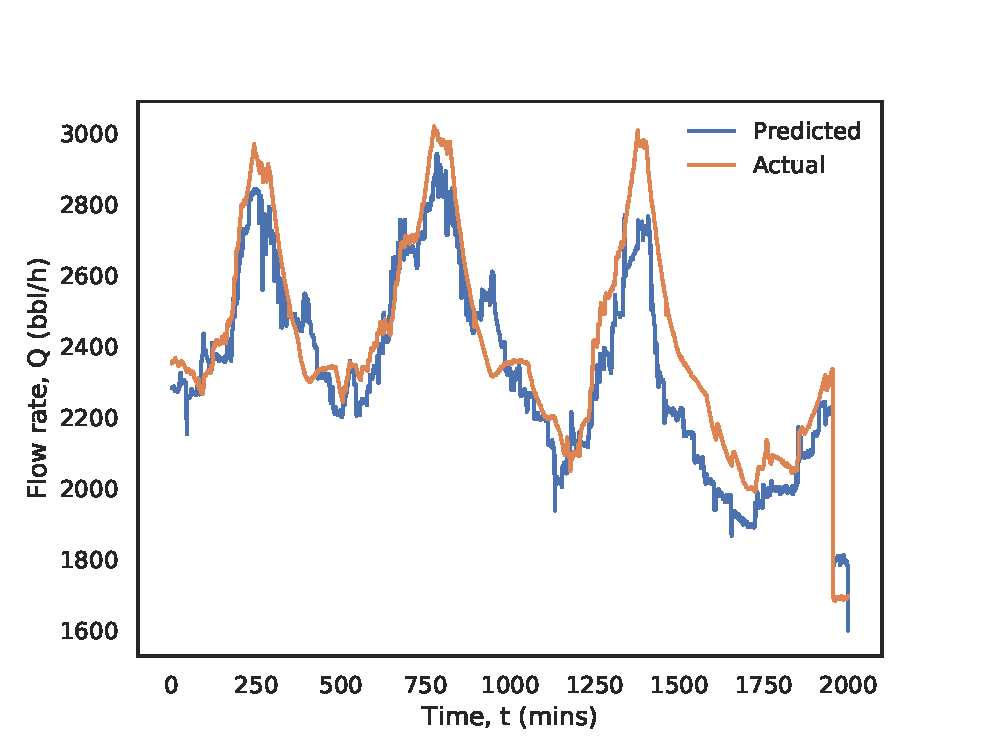
\includegraphics[width=\textwidth]{images/08quad_validation.eps}
         \caption{Predicted vs. actual flow rate for validation data using the quad. model.}
         \label{fig:08quad_validation}
     \end{subfigure}
     \begin{subfigure}[b]{0.45\textwidth}
         \centering
         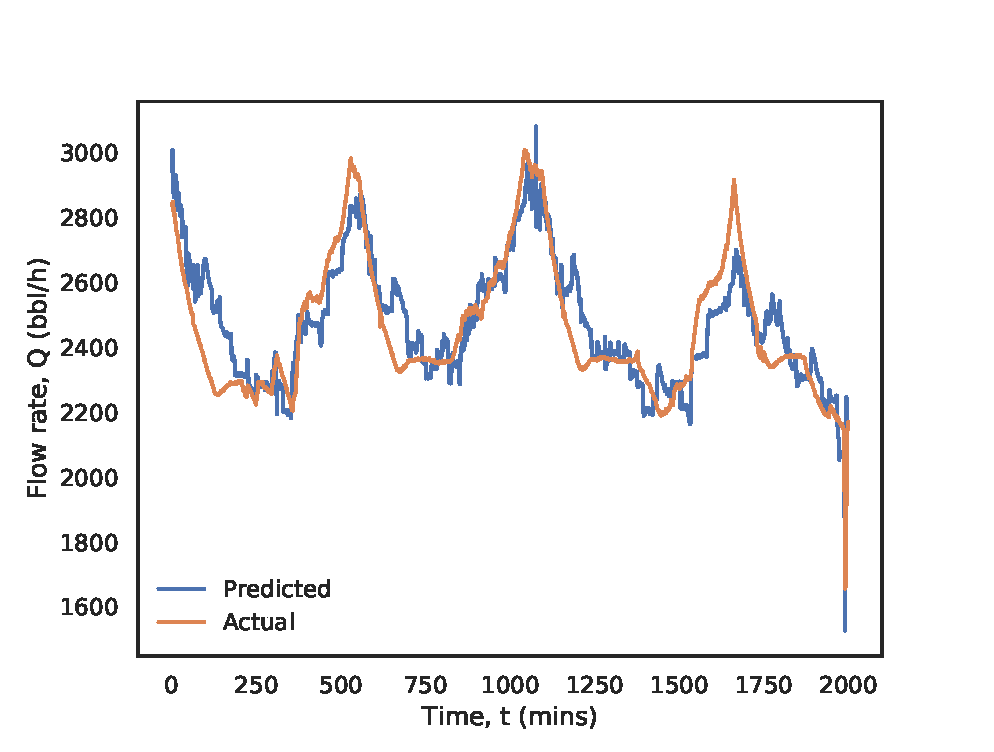
\includegraphics[width=\textwidth]{images/08quad_test.eps}
         \caption{Predicted vs. actual flow rate for the test data using the quadratic model.}
         \label{fig:08quad_test}
     \end{subfigure}
     \begin{subfigure}[b]{0.45\textwidth}
         \centering
         \includegraphics[width=\textwidth]{images/08sqrt_validation.eps}
         \caption{Predicted vs. actual flow rate for the validation data using the sqrt. model.}
         \label{fig:08sqrt_validation}
     \end{subfigure}
     \begin{subfigure}[b]{0.45\textwidth}
         \centering
         \includegraphics[width=\textwidth]{images/08sqrt_test.eps}
         \caption{Predicted vs. actual flow rate for the test data using the sqrt. model.}
         \label{fig:08sqrt_test}
     \end{subfigure}
        \caption{Polynomial regression validation and test plots.}
        \label{fig:08PolynomialPlots}
\end{figure}

%%%%%%%%%%%%%%%%%%%%%%%%%%%%%%%%%%%%%%%%%%%%%%%%%%%%%%%%%%%%%%%%%%%%%
%
% Neural Network Models
%
%%%%%%%%%%%%%%%%%%%%%%%%%%%%%%%%%%%%%%%%%%%%%%%%%%%%%%%%%%%%%%%%%%%%%
\noindent
\textit{Neural Network Models} \\
Neural networks are highly non-linear models that explore the individual and interaction effects of each variable with all other variables. The general structure of a neural network is shown in Figure \ref{fig:08NN}.  Neural networks are comprised of an input layer, some hidden layer(s), and an output layer.  The input layer consists of the input data, while the hidden layer(s) and output layer consists of fitted parameters, $W_{n_x \times n_b}$ and $b_{n_b \times 1}$. Here, $n_b$ and $n_x$ denotes the batch size and the dimension of the input layer, respectively. In Figure \ref{fig:08NN}, $x_m$ denotes the $m^{th}$ input variable.  The superscript and subscript of $a$ denotes the hidden layer number and the node number in the corresponding layer, respectively.  Subscript $m_1$ to $m_r$ denotes the number of nodes in hidden layers 1 to $r$, respectively.  Finally, superscript $o$ denotes the output layer.
\begin{figure}[h]
    \centering
    \includegraphics[width=0.9\textwidth]{images/08NN.png}
    \caption{Structure of a general neural network.}
    \label{fig:08NN}
\end{figure}

The details within a hidden layer's node is shown in Figure \ref{fig:08NNNode}. First, the outputs from the previous layer's nodes are inputted and multiplied by the weights of the current node.  The current node's bias is then added. If the current node is in the first layer, the outputs from the previous layer is replaced with the input variables. Afterwards, the output is sent to a rectified linear unit (ReLU) activation function given by:
\begin{equation}
    a^{[i]}_j=\begin{cases}
        y, & \text{if $y\geq0$}.\\
        0, & \text{otherwise}.
    \end{cases}
    \label{eq:08ReLU}
\end{equation}
where $i$ and $j$ denotes any hidden layer and any node number, respectively.  
\begin{figure}[h]
    \centering
    \includegraphics[width=0.3\textwidth]{images/08NNNode.png}
    \caption{Inside a hidden layer's node.}
    \label{fig:08NNNode}
\end{figure}

Mathematically, for one example $x$:
\begin{center}
    $z^{[1]}_j = W^{[1]}x + b^{[1]}$ \\
    $a^{[1]}_j = ReLU(z^{[1]}_j)$ \\
    $z^{[2]}_j = W^{[2]}a^{[1]}_j + b^{[2]}$ \\
    $a^{[2]}_j = ReLU(z^{[2]}_j)$ \\
    ... \\
    $z^{[r]}_j = W^{[r]}a^{[r - 1]}_j + b^{[r]}$ \\
    $a^{[r]}_j = ReLU(z^{[r]}_j)$ \\
    $y = W^{[o]}a^{[r]}_j + b^{[o]}$ \\  
\end{center}

The hyper parameters for each neural network is given in Table \ref{tab:08NN_hp}. $\lambda$ was increased as the neural network got more complex to reduce overfitting.  The ReLU activation function was chosen for computational efficiency and avoiding the exploding/vanishing gradient problem \cite{ReLU}.
\begin{table}[h]
    \centering
    {\setstretch{1.2}
    \begin{tabular}{ c | c | c | c}
        Hyper Parameter                            &  Small NN  &  Med. NN  & Large NN       \\
        \hline
        Epochs                                     &  700       & 1000      & 1200  \\
        Minibatch size                             &  8192      & 8192      & 8192  \\
        Learning rate, $\alpha$                    &  0.001     & 0.001     & 0.001 \\
        Regularization, $\lambda$                  &  0.001     & 0.003     & 0.005 \\
        Number of layers                           &  3         & 6         & 8     \\
        Neurons per layer                          &  20        & 30        & 40    \\
        Activation function for hidden layers      & ReLU       & ReLU      & ReLU  \\
    \end{tabular}}
    \caption{Hyper parameters for the feed-forward neural network.}
    \label{tab:08NN_hp}
\end{table}

Table \ref{tab:08_nn} shows the performance assessment of the small, medium and large neural networks.  In all cases, the training and validation data set performance was significantly better compared to the linear model; however, the performance was only slightly better on the test data set. On the training and validation data, the error went down by up to 61\%.  On the test data, error went down by up to 19\%. The difference may be caused by the test data being different from the training data.  Due to the complexity of neural network models, they perform exceptionally well on data that shares similar characteristics as the training data, but perform poorly otherwise. To close the gap in performance, a higher $\lambda$ could be used to reduce model complexity.  Moreover, smaller neural networks could also be explored to reduce model complexity.

\begin{table}[h]
\centering
{\setstretch{1.2}
\begin{tabular}{c|c|c|c|c|c|c|c|c|c|}
\multicolumn{1}{l|}{} & \multicolumn{3}{c|}{Training Data}                                               & \multicolumn{3}{c|}{Validation Data}                                             & \multicolumn{3}{c|}{Test Data}                                                   \\ \cline{2-10} 
\multicolumn{1}{l|}{} & \multicolumn{1}{c|}{Sm.} & \multicolumn{1}{c|}{Med.} & \multicolumn{1}{c|}{Lar.} & \multicolumn{1}{c|}{Sm.} & \multicolumn{1}{c|}{Med.} & \multicolumn{1}{c|}{Lar.} & \multicolumn{1}{c|}{Sm.} & \multicolumn{1}{c|}{Med.} & \multicolumn{1}{c|}{Lar.} \\ \hline
MAE                   & 48                       & 42                        & 38                        & 50                       & 45                        & 37                        & 87                       & 87                        & 91                        \\
RMSE                  & 66                       & 58                        & 57                        & 69                       & 61                        & 56                        & 117                      & 107                       & 118                       \\
\end{tabular}}
    \caption{Performance assessment of the neural network models.}
    \label{tab:08_nn}
\end{table}

The comparison of actual and predicted flow rates on the validation and test data for the neural nets are shown in Figures \ref{fig:08smallnn_valid} to \ref{fig:08largenn_test}.  

\begin{figure}[p]
     \centering
     \begin{subfigure}[b]{0.48\textwidth}
         \includegraphics[width=\textwidth]{images/08smallnn_valid.eps}
         \caption{Predicted vs. actual flow rate for validation data using the small neural net.}
         \label{fig:08smallnn_valid}
     \end{subfigure}
     \begin{subfigure}[b]{0.48\textwidth}
         \includegraphics[width=\textwidth]{images/08smallnn_test.eps}
         \caption{Predicted vs. actual flow rate for the test data using the small neural net.}
         \label{fig:08smallnn_test}
     \end{subfigure}
     \begin{subfigure}[b]{0.48\textwidth}
         \includegraphics[width=\textwidth]{images/08mednn_valid.eps}
         \caption{Predicted vs. actual flow rate for the validation data using the med. neural net.}
         \label{fig:08mednn_valid}
     \end{subfigure}
     \begin{subfigure}[b]{0.48\textwidth}
         \includegraphics[width=\textwidth]{images/08mednn_test.eps}
         \caption{Predicted vs. actual flow rate for the test data using the med. neural net.}
         \label{fig:08mednn_test}
     \end{subfigure}
     \begin{subfigure}[b]{0.48\textwidth}
         \includegraphics[width=\textwidth]{images/08largenn_valid.eps}
         \caption{Predicted vs. actual flow rate for the validation data using the large neural net.}
         \label{fig:08largenn_valid}
     \end{subfigure}
     \begin{subfigure}[b]{0.48\textwidth}
         \includegraphics[width=\textwidth]{images/08largenn_test.eps}
         \caption{Predicted vs. actual flow rate for the test data using the large neural net.}
         \label{fig:08largenn_test}
     \end{subfigure}
        \caption{Feed-forward neural network validation and test plots.}
        \label{fig:08PolynomialPlots}
\end{figure}

%%%%%%%%%%%%%%%%%%%%%%%%%%%%%%%%%%%%%%%%%%%%%%%%%%%%%%%%%%%%%%%%%%%%%
%
% LPV MODELS
%
%%%%%%%%%%%%%%%%%%%%%%%%%%%%%%%%%%%%%%%%%%%%%%%%%%%%%%%%%%%%%%%%%%%%%
\noindent
\textit{Linear Parameter-varying Models} \\
Lastly, the linear parameter-varying model (LPV) was explored to model the pipeline. It is clear that the process is non-linear due to the increase in accuracy when switching to a non-linear model structure. LPV models were selected due to their non-linear nature while still retaining the interpretability of linear models. Furthermore, any non-linear model can be approximated by a set of linear models \cite{LPV}. The LPV model is given by:
\begin{equation}
    \begin{split}
        \hat{y} = W_{1, 1}^Tx + W_{1, 2}^Tu + b_1 \\
        \hat{y} = W_{2, 1}^Tx + W_{2, 2}^Tu+ b_2 \\
        ... \\
        \hat{y} = W_{n, 1}^Tx + W_{n, 2}^Tu + b_n \\
    \end{split}
    \label{eq:08LPV_structure}
\end{equation}
where $n \geq 1$ represents the number of linear models used to capture the data set. Here, $W_n$ and $b_n$ are the weights and biases corresponding to the $n^{th}$ model, respectively. For this study, $n=2$.  The models corresponded to the two clusters identified in Figure \ref{fig:08DBSCAN}.  Models 1 and 2 are identified from clusters 1 and 2, respectively.  The hyper parameters for models 1 and 2 are identical to the previous linear models, and are shown in Table \ref{tab:08LSHparameters}. During online implementation, the model will be selected based on the Euclidean distance between the features of the new data and the centroid of the two clusters.  However, if the distance exceeds 1.15 in both cases, the data will be labeled as anomalous.

The performance assessment of the two LPV models are shown in Table \ref{tab:08cluster1_cluster2_reg}. Overall, the LPV models were able to reduce modelling error compared to normal linear regression. Model 1 was only used to predict high flow rate scenarios. Nevertheless, its MAE and RMSE were still 8\% lower compared to the linear regression model used to predict for all data.  For model 2, the MAE and RMSE were up to 31\% lower. 

\begin{table}[h]
    \centering
    {\setstretch{1.2}
    \begin{tabular}{c|c|c|c|c|c|c|}
      & \multicolumn{2}{c|}{Training data} & \multicolumn{2}{c|}{Validation data} & \multicolumn{2}{c|}{Test data} \\ \cline{2-7} 
      & Cl. 1            & Cl. 2           & Cl. 1             & Cl. 2            & Cl. 1          & Cl. 2         \\ \hline
    MAE   & 90               & 66              & 90                & 67               & 96             & 85            \\
    RMSE  & 115              & 91              & 116               & 92               & 120            & 110           \\
    $R^2$ & 0.87             & 0.90            & 0.86              & 0.89             & 0.78           & 0.57         
    \end{tabular}}
    \caption{Performance assessment for clusters 1 and 2 regression models.}
    \label{tab:08cluster1_cluster2_reg}
\end{table}

The comparison of actual and predicted flow rates on the validation and test data for the LPV models are shown in Figures \ref{fig:08cluster1_valid} to \ref{fig:08cluster2_test}. In Figures \ref{cluster2_valid} and \ref{cluster2_test}, it can be seen that model 2 performs poorly on the data.  This might be caused by some unobserved variables that are only applicable for low flow rate operations.
\begin{figure}[h]
    \centering
     \begin{subfigure}[b]{0.48\textwidth}
         \includegraphics[width=\textwidth]{images/08cluster1_valid.eps}
         \caption{Predicted vs. actual flow rate for validation data using model 1.}
         \label{fig:08cluster1_valid}
     \end{subfigure}
     \begin{subfigure}[b]{0.48\textwidth}
         \includegraphics[width=\textwidth]{images/08cluster1_test.eps}
         \caption{Predicted vs. actual flow rate for the test data using model 1.}
         \label{fig:08cluster1_test}
     \end{subfigure}
     \begin{subfigure}[b]{0.48\textwidth}
         \includegraphics[width=\textwidth]{images/08cluster2_valid.eps}
         \caption{Predicted vs. actual flow rate for the validation data using model 2.}
         \label{fig:08cluster2_valid}
     \end{subfigure}
     \begin{subfigure}[b]{0.48\textwidth}
         \includegraphics[width=\textwidth]{images/08cluster2_test.eps}
         \caption{Predicted vs. actual flow rate for the test data using model 2.}
         \label{fig:08cluster2_test}
     \end{subfigure}
        \caption{Linear parameter-varying models' validation and test plots.}
        \label{fig:08PolynomialPlots}
\end{figure}

Ultimately, the LPV model structure was selected to model the pipeline.  The LPV model has the interpretability of linear models, while having the predictive capabilities of non-linear models.  Furthermore, the LPV model identifies a separate set of parameters for the two distributions, making the optimization algorithm more representative of live operations.  For example, because no DRA was used for lower flow rates, the optimization algorithm will have explicit constraints on model 2 to not use DRA as well. A similar example would be using only Ault booster 1 for cluster 2, while using Ault booster 2 for cluster 1.  The advantages of these constraints are twofold: i) More realistic to live operations.  ii) Avoid model extrapolations (since no DRA data was used to identify model 2, the optimizer should not be able to use it for optimization).

\subsubsection{Time-series Modelling}
All previous models are static (i.e., $y_{ss} = f(x, u)$) and are used for the real time optimization layer in Figure \ref{fig:08APC}. To completely automate the pipeline operations, a dynamic model was identified for the application of supervisory control. In dynamic modelling, temporal correlations within the time-series data are exploited to improve model accuracy.  Moreover, $y_t$ is measured at each time and can be used to further improve model accuracy. The time-series model will have the following structure:
\begin{equation}
    y_{t+1} = f(x_{t}, x_{t - 1}, ..., x_{t-p}, u_{t}, u_{t - 1}, ..., u_{t - q}, y_{r})
\end{equation}
Here, subscripts $p$ and $q$ denote the number of previous states and inputs to be considered in the model, respectively.  Subscript $r = max(p, q)$. Least squares will be used to identify the time-series model with data augmented as $[x_t, u_t | x_{t - 1}, u_{t - 1} | ... ]$.  After exploring a variety of $p$'s and $q$'s, the final hyper parameters used for the time series model is shown in Table \ref{tab:08ts_parameters}.
\begin{table}[h]
    \centering
    {\setstretch{1.2}
    \begin{tabular}{ c | c}
        Hyper Parameter                  &  Value       \\
        \hline
        Epochs                           &  1000      \\
        Minibatch size                   &  8192     \\
        Learning rate, $\alpha$          &  0.001    \\
        Regularization, $\lambda$        &  0.001    \\
        $\#$ of previous states, $p$     &  2  \\
        $\#$ of previous inputs, $q$     &  2  \\
    \end{tabular}}
    \caption{Hyper parameters for the time-series least squares model.}
    \label{tab:08ts_parameters}
\end{table}

The performance metrics of the time-series model is shown in Table \ref{tab:08ts_performance}.  Compared to static models, dynamic models are significantly more accurate; error metrics went down by up to 87\%.
\begin{table}[h]
    \centering
    {\setstretch{1.2}
    \begin{tabular}{ c | c | c | c}
                             &  Training data    &  Validation data   &    Test data      \\
        \hline
        MAE                  &      22           &        17          &   25    \\
        RMSE                 &      41           &        34          &   65    \\ 
        $R^2$                &      0.99         &        0.99        &   0.86  \\
    \end{tabular}}
    \caption{Performance assessment for the time-series least squares model.}
    \label{tab:08ts_performance}
\end{table}

The comparison of actual and predicted flow rates on the validation and test data for the time-series least square model are shown in Figure \ref{fig:08ts_ls}. 
\begin{figure}[h]
    \centering
     \begin{subfigure}[b]{0.48\textwidth}
         \includegraphics[width=\textwidth]{images/08ts_validation.eps}
         \caption{Validation data.}
         \label{fig:08ts_valid}
     \end{subfigure}
     \begin{subfigure}[b]{0.48\textwidth}
         \includegraphics[width=\textwidth]{images/08ts_test.eps}
         \caption{Test data.}
         \label{fig:08ts_test}
     \end{subfigure}
        \caption{Predicted vs. actual flow rate using the time-series model.}
        \label{fig:08ts_ls}
\end{figure}


\subsubsection{Model Applicability Range}
Extrapolation while using data-driven models introduce risks to operations. Thus, Table \ref{tab:08StateConst} shows the ranges of states where the model is most effective. The ranges were identified from the historical data. Usage of the models beyond the normal range may be ineffective.

\begin{table}[h]
    \centering
    {\setstretch{1.2}
    \begin{tabular}{ p{5cm} | c }
        Variables                         &  Valid Range           \\
        \hline
        Flow Rate (bbl/h)                       &      1500 - 3050       \\
        Cheyenne Density (API)                  &      22 - 47           \\ 
        CIG Density (API)                       &      15 - 47           \\
        Ault Density (API)                      &      15 - 50           \\
        Cheyenne Temp (°C)                      &      35 - 50           \\
        CIG Temp (°C)                           &      41 - 51           \\
        Ault Temp (°C)                          &      43 - 54           \\
        Fort Lupton Temp (°C)                   &      46 - 60           \\
        Commerce City Temp  (°C)                &      48 - 60           \\
    \end{tabular}}
    \caption{Applicable states of the machine learning models.}
    \label{tab:08StateConst}
\end{table}

In addition to the state ranges provided above, the recommended set points are also limited to avoid extrapolation.  The set point ranges are shown in Table \ref{tab:08InputConst}.

\begin{table}[h]
    \centering
    {\setstretch{1.2}
    \begin{tabular}{ p{6cm} | c }
        Variables                               &  Valid Range            \\
        \hline
        Cheyenne VFD (Amps)                     &      100 - 340          \\
        Fort Lupton VFD (Amps)                  &      60 - 145           \\ 
        CIG \& Ault Sweet DRA (ppm)             &      20 - 40            \\
        CIG \& Ault Sour DRA (ppm)              &      20 - 40            \\
    \end{tabular}}
    \caption{Applicable inputs of the machine learning models.}
    \label{tab:08InputConst}
\end{table}

\subsubsection{Adaptive Machine Learning}
\paragraph{Online Learning vs. Incremental Learning}
\paragraph{ART: Adaptive Resonance Theory}
\paragraph{Implementation of Adaptive Machine Learning}

\begin{figure}
    \centering
    \includegraphics[width=\textwidth]{images/08IncrementalLearning.png}
    \caption{Importance Sampling Incremental Supervised learning architecture.}
    \label{fig:08ART}
\end{figure}

\subsection{Mixed Integer Linear Programming}
The information flow of the optimization algorithm is shown in Figure \ref{fig:08Optimization_flow}.  First, a desired flow will be inputted by the operators depending on the demand from Commerce City.  Then, the machine learning model along with equality and in-equality constraints will be provided to the mixed integer linear program (MILP).  Given the objective function, decision variables, and the current costs, the MILP will finally output the optimal set points.
\begin{figure}[h]
    \centering
    \includegraphics[width=\textwidth]{images/08Optimization_flow.png}
    \caption{Optimization information flow chart.}
    \label{fig:08Optimization_flow}
\end{figure}

\noindent
\textit{Mixed Integer Linear Program} \\
MILP was used to perform steady state optimization on the linear model because the decision variables included binary and continuous variables.  In total, there was 10 decision variables; 4 binary and 6 continuous.  The binary and continuous variables are shown in Table \ref{tab:08binary_cont}.

\begin{table}[h]
    \centering
    {\setstretch{1.2}
    \begin{tabular}{ c | c }
        Binary                       &  Continuous           \\
        \hline
        On/off Cheyenne Pump               &  Cheyenne \& Fort Lupton VFD            \\
        2$\times$ On/off Ault Pump         &  2$\times$ Sweet \& 2$\times$ Sour DRA  \\
        On/off Fort Lupton Pump
    \end{tabular}}
    \caption{Binary and continuous decision variables.}
    \label{tab:08binary_cont}
\end{table}

\noindent
\textit{Constraints} \\
The constraints are the machine learning model, equality, and in-equality constraints.  The equality and in-equality constraints are shown in Table \ref{tab:08eq_neq_constraints}. From the data provided, the Cheyenne pump was on 95\% of the time, and at least one Ault on/off pump was always on. Therefore, constraints were incorporated to reflect this.  Additionally, constraints were used to ensure proper DRA was injected into the pipeline for the different crudes.  There were also pressure constraints on the outlet pressure of the pumps to ensure safe operations.  Before a recommendation is made to the operators, the set points are used to predict for the outlet pressures at each pump to ensure they do not exceed the maximum allowable working pressure (MAWP). Finally, the flow rate is given a range to ensure optimization feasibility. Specifying exact flow rates lead to infeasible solutions because there may not exist a combination to get an \textit{exact} flow rate.

\begin{table}[h]
    \centering
    {\setstretch{1.5}
    \begin{tabular}{c|c}
         Equality Constraints              & In-equality Constraints \\
         \hline
         On/off Cheyenne Pump = On         & $\text{Lower bound} \leq \text{Flow rate} \leq \text{Upper bound}$ \\
         
         Ault Pump 1 and/or 2 = On          & $P_{Outlet}^{Chey} \leq 1480 \text{ psi}$       \\
         
         $API^{CIG} \geq 30: DRA_{Sweet}^{CIG}$ = On & $P_{Outlet}^{Ault} \leq 1613 \text{ psi}$ \\
         
         $API^{CIG} \leq 30: DRA_{Sour}^{CIG}$ = On  & $P_{Outlet}^{FL} \leq 1613 \text{ psi}$  \\
         
         $API^{Ault} \geq 30: DRA_{Sweet}^{Ault}$ = On & $20 \text{ ppm} \leq DRA \leq 40 \text{ ppm}$                 \\
         
         $API^{Ault} \leq 30: DRA_{Sour}^{Ault}$  = On  & $100 \text{ Amps} \leq VFD^{Chey} \leq 340 \text{ Amps}$   \\
         
         Cheyenne On/off = 28 Amps  & $60 \text{ Amps} \leq VFD^{FL} \leq 145 \text{ Amps}$  \\
         Ault 1 Pump = 190 Amps & \\
         Ault 2 Pump = 278 Amps & \\
         Fort Lupton Pump = 117 & \\
    \end{tabular}}   
    \caption{List of equality and inequality constraints}
    \label{tab:08eq_neq_constraints}
\end{table}

Pressure models were built to ensure MAWP was not exceeded when the recommended set points are implemented. In the end, three linear regression pressure models were identified; each at the outlet of a pump station (Cheyenne, Ault, Fort Lupton) where pressure is expected to be the highest. The inputs to the pressure models were all upstream of the pump station is located and is given in Table \ref{tab:08pressure_inputs}.

\begin{table}[]
    \centering
    {\setstretch{1.2}
    \begin{tabular}{p{5cm} | p{5cm} | p{5cm}}
         Cheyenne & Ault & Fort Lupton \\
         \hline
         
         Pipeline inlet pressure & Pipeline inlet pressure & Pipeline inlet pressure \\
         
         Cheyenne VFD & Cheyenne VFD & Cheyenne VFD \\
         
         Cheyenne on/off pump & Cheyenne on/off pump & Cheyenne on/off pump \\
         
         Cheyenne temperature & Ault on/off pump 1 & CIG DRA ppm \\
         
         & Ault on/off pump 2 & Ault on/off pump 1 \\
         
         & CIG DRA ppm & Ault on/off pump 2 \\
         
         & Cheyenne temperature & Ault DRA ppm \\
         
         & Ault temperature & Fort Lupton VFD \\
         & & Fort Lupton on/off pump \\
         & & Cheyenne temperature \\
         & & Ault temperature \\
         & & FL temperature \\
    \end{tabular}}
    \caption{Inputs to the pressure constraint models.}
    \label{tab:08pressure_inputs}
\end{table}

The performance assessment of the Cheyenne, Ault, and Fort Lupton pressure constraint models are shown in Table \ref{tab:08pres_const_performance}. The Cheyenne pressure prediction is very accurate; however the accuracy decreases as we traverse down the pipeline.  The primary reason is because an accurate inlet pressure is required to predict for the outlet pressure.  But the inlet pressure beyond Cheyenne is unknown because the set points are not actuated in the pipeline yet. Furthermore, predicting the outlet pressure at Ault is especially difficult because a mechanism exists to limit the pressure to 1377 psi.  The mechanism's data is not captured, and causes the regression curve to be hard constrained at an upper bound. Consequently, this causes many inputs to result in the same output, and hinders learning.

\begin{table}[h]
    \centering
    {\setstretch{1.2}
    \begin{tabular}{c|c|c|c|c|c|c|}
    \multicolumn{1}{l|}{} & \multicolumn{3}{c|}{Training Data} & \multicolumn{3}{c|}{Validation Data} \\ \cline{2-7} 
    \multicolumn{1}{l|}{} & Cheyenne   & Ault   & Fort Lupton  & Cheyenne    & Ault   & Fort Lupton   \\ \hline
    MAE                   & 75         & 179    & 25           & 72          & 179    & 27            \\
    RMSE                  & 101        & 217    & 32           & 96          & 217    & 35            \\
    $R^2$                 & 0.88       & 0.5    & 0.47         & 0.89        & 0.49   & 0.46         
    \end{tabular}}
    \caption{Performance assessment of the Cheyenne, Ault, and Fort Lupton pressure constraint models}
    \label{tab:08pres_const_performance}
\end{table}

The performance of the pressure constraint models on the validation data is shown in Figures \ref{fig:08Chey_Pconst} to \ref{fig:08FL_Pconst}.

\begin{figure}
    \centering
    \begin{subfigure}[b]{0.325\textwidth}
         \centering
         \includegraphics[width=\textwidth]{images/08Chey_Pconst.eps}
         \caption{Cheyenne}
         \label{fig:08Chey_Pconst}
    \end{subfigure}
    \begin{subfigure}[b]{0.325\textwidth}
         \centering
         \includegraphics[width=\textwidth]{images/08Ault_Pconst.eps}
         \caption{Ault}
         \label{fig:08Ault_Pconst}
    \end{subfigure}
    \begin{subfigure}[b]{0.325\textwidth}
         \centering
         \includegraphics[width=\textwidth]{images/08FL_Pconst.eps}
         \caption{Fort Lupton}
         \label{fig:08FL_Pconst}
    \end{subfigure}
    \caption{Pressure constraint model performance on validation data.}
    \label{fig:08Pconst}
\end{figure}

\noindent
\textit{Objective Function, Costs and Decision Variables} \\
The objective is to operate the pipeline at the desired flow rate with the minimum possible operating cost.  The optimization is given by:

\begin{mini*}|s|
    {J} {= \left[ \alpha_i \sum_i \mu_i \cdot DRA_i + \beta \sum_j \nu_j \cdot I_jV_j \right]}
    {}{}
    \addConstraint{y = f(x, u)}                
    \addConstraint{\nu_{Ault1} + \nu_{Ault2} \geq 1} 
    \addConstraint{\nu_{Chey} = 1} 
    \addConstraint{20 \leq DRA_i \leq 40, \; i \in I} 
    \addConstraint{\gamma_j^{min} \leq I_j \leq \gamma_j^{max}, \; j \in J}{}
\end{mini*}
where $\alpha$ denotes the cost of DRA per ppm, $\beta$ denotes the cost of one kWh, $mu$ denotes the on/off status of the DRA pumps, and $\nu$ denotes the on/off status of the pumps. $DRA_i$ is the DRA ppm set point of the $i^{th}$ DRA injection pump. Moreover, $V_j$ and $I_j$ are the voltage and drawn amperes corresponding to the $j^{th}$ pump. Here, $\gamma_j$ are the upper and lower bounds of the VFDs' currents and are provided in Table \ref{tab:08eq_neq_constraints}. For on/off pumps, $\gamma_j$ is fixed.

The voltages of the pumps are provided in Table \ref{tab:08Voltages}.  The power cost per kWh for the pipeline was \$0.09 USD.
\begin{table}[h]
    \centering
    {\setstretch{1.2}
    \begin{tabular}{c|c}
        Pump          &  Voltage \\
        \hline
        $VFD^{Chey}$    &  4160    \\
        $VFD^{FL}$      &  4160    \\
        On/off $Pump^{Chey}$    & 480   \\
        On/off $Pump^{Ault1}$   & 4000  \\
        On/off $Pump^{Ault2}$   & 4000  \\
        On/off $Pump^{FL}$      & 480   \\
    \end{tabular}}
    \caption{Voltages for the pumps.}
    \label{tab:08Voltages}
\end{table}

The cost to increase DRA ppm is dependent on the flow rate of the pipeline. Higher flow rates require more DRA to be injected; hence a higher cost.  The cost curves for DRA is shown in Figures \ref{fig:08DRA_Cost}.  Given a flow rate, the cost to increase the DRA ppm is given by Equations \ref{eq:08sweet_dra} and \ref{eq:08sour_dra} for the sweet and sour DRA, respectively.

\begin{figure}[h]
    \centering
    \includegraphics[width=\textwidth]{images/08DRA_Cost.png}
    \caption{Cost of DRA as a function of flow rate.}
    \label{fig:08DRA_Cost}
\end{figure}

\begin{equation}
    \$ / ppm_{sweet} = 0.00071Q + 0.01630
    \label{eq:08sweet_dra}
\end{equation}
\begin{equation}
    \$ / ppm_{sour} = 0.00176Q + 0.00226
    \label{eq:08sour_dra}
\end{equation}
where Q denotes the volumetric flow rate in barrels per hour.

\subsection{Conceptual Software Design}
The conceptual software design for the optimization product is shown in Figure \ref{fig:08concept_software}. First, the users populate the costs corresponding to each equipment.  The pump costs are on a \$ per kWh basis, and the DRA cost is based on \$ per ppm. Operating costs can also be incorporated by multiplying the costs by a fixed factor (e.g. 1.1 $\cdot$ \$/kWh). Currently, DRA costs are automatically calculated based on Equations \ref{eq:08sweet_dra} and \ref{eq:08sour_dra}. Next, the user specifies the maximum steady state operating pressure (MSSOP) for the pipeline, and enter the desired flow rate.  Finally, the "OPTIMIZE" button is pressed and all the boxes outlined in green will be populated with the optimal steady state.  When a steady state is no longer deemed optimal, the outline will become red.  An example of such a scenario would be when the batch switches from sweet to sour.  During maintenance activities, the user can click the "ADVANCED..." button, specify special constraints and eliminate equipment from the optimization. For example, if the Cheyenne VFD is under maintenance, $\nu_{Chey VFD}$ can be switched to 0 to prevent the optimization from using it.

\begin{figure}[h]
    \centering
    \includegraphics[width=\textwidth]{images/08conceptual_software.pdf}
    \caption{Conceptual software design for the optimization tool.}
    \label{fig:08concept_software}
\end{figure}

A flow diagram of the inner workings of the product is shown in Figure \ref{fig:08Product_Flow}.

\begin{figure}[h]
    \centering
    \includegraphics[width=\textwidth]{images/08Product_Flow.png}
    \caption{Internal flow diagram of the product.}
    \label{fig:08concept_software}
\end{figure}

\subsection{Cost Savings and Impact on Society}


% \chapter{RL Accelerated Economic MPC}
% \input{chapters/Chapter09:RLandEMPC.tex}

% \chapter{Automated Tuning using RL}
% \input{chapters/Chapter10:RLTuning.tex}

\chapter{Concluding Remarks}
- RL is excellent in an highly mathematical complex problem that you have a simulator for like games.  But such processes don't exist in real life.
- MPC is the ideal outcome of RL everytime.
- RL has more exotic applications than control, and its value is most likely not in control.

\printbibliography

\appendix
\chapter{testing}

\chapter{testing 32}


\end{document}